%&TeX spellcheck = it_IT
\documentclass[12pt,a4paper,twoside]{report}
\usepackage{geometry}%to cus­tomize page lay­out
\usepackage[italian]{babel}%man­ages cul­tur­ally-de­ter­mined ty­po­graph­i­cal (and other) rules, and hy­phen­ation pat­terns
\usepackage[T1]{fontenc}%perchè faccia per bene i caratteri accentati nell'output
\usepackage[utf8]{inputenc}%perchè riconosca i caratteri accentati nel sorgente tex
\usepackage[hyphens]{url}%per inserire url
\usepackage{fancyhdr}%per header e foooter
\usepackage{graphicx}%per le immagini
\usepackage{wrapfig}%to wrap images with text
%\usepackage{epsfig}
\usepackage{amsthm}
\usepackage{listings}%per inserie codice sorgente
\usepackage{xcolor}%colori! :D
\usepackage{amsmath}%per formule matematiche
\usepackage{amssymb} %simboli matematici
\usepackage{booktabs}%en­hances the qual­ity of ta­bles
\usepackage{caption}%to cus­tomise the cap­tions in float­ing en­vi­ron­ments like fig­ure and ta­ble
% \usepackage{subfig}%manipulation and ref­er­ence of small or ‘sub’ fig­ures and ta­bles within a sin­gle fig­ure or ta­ble en­vi­ron­ment
\usepackage{eurosym}%The Euro­pean cur­rency sym­bol for the Euro
\usepackage{siunitx}%tante cose sulle unità di misura
\usepackage{calligra}%cal­li­graphic font
\usepackage{verbatim}
\usepackage{indentfirst}%Indent first paragraph after section header
\usepackage{microtype}%fa diventare i font più belli
\usepackage{lmodern}%fontbelli
\usepackage{braket}%parentesi
\usepackage{mathtools}%to en­hance the ap­pear­ance of doc­u­ments con­tain­ing a lot of math­e­mat­ics
\usepackage{mathrsfs}  %per fare le lettere calligrafiche
\usepackage{bm}%define \bm{} that makes the argument bold
\usepackage{empheq}%markup per le formule di amsmath
\usepackage{pstricks}%macros for gen­er­at­ing PostScript that is us­able with most TeX macro for­mats
\usepackage{emptypage}%toglie il numero di pagina alle pahine create con clearpage e cleardoublepage
\usepackage{todonotes}
\usepackage{textcomp}%per il simbolo dei gradi
\usepackage{enumitem}%per controllare gli spazi nelle liste
\usepackage{pbox}%per fare celle con più linee nelle tabelle
\usepackage{placeins}%con \FloatBarrier mette il testo dopo le cose float
\usepackage{longtable}%per tabelle che vanno da una pagina all'altra
\usepackage[final]{pdfpages}%per importare pdf
\usepackage{tkz-graph}
\usepackage{multirow}
\usepackage{float}
\usepackage{subcaption}


%fine pacchetti

%:::::::::::::::::::::IMPOSTAZIONI::::::::::::::::::::::::::::::::::::::::::::::::::::::::::::::::::::

\geometry{a4paper,top=85pt,bottom=85pt,left=127pt,right=127pt} %imposto la geometria del documento
\captionsetup{tableposition=top,figureposition=bottom,font=small}  %impostazione dei caption di immagini e tabelle
%\DeclareCaptionFormat{elaborazione}{#1#2#3\par}

%::::::::::::::::::::::::::::::::::::::::::::::::::::::::::::::::::::::::::::::::::::::::::::::::::::


\begin{document}

%::::::::::::::::::::::::::DEFINIZIONI DI COMANDI::::::::::::::::::::::::::::::::::::::::::::::::::::
\newcommand{\whitePage}{\cleardoublepage} % pagina bianca e rende la successiva una pagina destra

\newcommand{\HRule}{\rule{\linewidth}{0.6mm}} % command for the horizontal lines, change thickness here

\newcommand*{\eupgrave}{\MakeUppercase{è}} % maiuscola è accentata
%fine comandi
%::::::::::::::::::::::::::::::::::::::::::::::::::::::::::::::::::::::::::::::::::::::::::::::::::::



%::::::::::::::::::::::::::IMPOSTAZIONI GLOBALI::::::::::::::::::::::::::::::::::::::::::::::::::::::
% \setlist(nosep)
%::::::::::::::::::::::::::::::::::::::::::::::::::::::::::::::::::::::::::::::::::::::::::::::::::::


%::::::::::::::::::::::::::::::::TITLE PAGE::::::::::::::::::::::::::::::::::::::::::::::::::::::::::
\begin{titlepage}



\center  % Center everything on the page

\textsc{\Large \\[4.5cm]Università degli Studi di Padova}\\[1.5cm]
\textsc{\Large Corso di laurea triennale in Ingegneria dell'Informazione}\\[0.5cm]

\noindent\rule{\textwidth}{0.6pt}\\[0.4cm]
{ \Large{\bfseries Analisi di una rete di autori di pubblicazioni scientifiche}}\\[0.4cm]
\noindent\rule{\textwidth}{0.6pt}\\[1cm]


\includegraphics[height=4cm]{img/unipd-bn}\\[1cm]


\begin{minipage}{0.4\textwidth}
\begin{flushleft} \large
\emph{Laureando:}\\
Pietro Maria \textsc{Nobili} % Your name
\end{flushleft}
\begin{flushleft} \large
\emph{Matricola:}\\
1067941 % Your number
\end{flushleft}
\end{minipage}
~
\begin{minipage}{0.5\textwidth}
\begin{flushright} \large
\emph{Relatore:} \\
Prof.ssa Cinzia \textsc{Pizzi} \\% Supervisor's Name
\end{flushright}
\begin{flushright} \large
\emph{Correlatore:} \\
Dott. Mattia \textsc{Samory} % Supervisor's Name
\end{flushright}
\end{minipage}\\[2cm]


{\large 18 Luglio 2018}\\
{\large Anno Accademico 2017/2018}\\[3cm] % Date, change the \today to a set date if you want to be precise


\vfill % Fill the rest of the page with whitespace

\end{titlepage}
%::::::::::::::::::::::::::::::::::::::::::::::::::::::::::::::::::::::::::::::::::::::::::::::::::::


\whitePage

%::::::::::::::::::::::::::::::::::INDEX:::::::::::::::::::::::::::::::::::::::::::::::::::::::::::::

\pagenumbering{Roman}
\tableofcontents

%::::::::::::::::::::::::::::::::::::::::::::::::::::::::::::::::::::::::::::::::::::::::::::::::::::



%::::::::::::::::::::::::::::::::::THE REAL CONTENT::::::::::::::::::::::::::::::::::::::::::::::::::

\whitePage



\newpage
\pagenumbering{arabic}
\setcounter{page}{1}
\section*{Abstract} \label{abstract} % the asterisk is to remove the numbering
\addcontentsline{toc}{chapter}{Abstract} % we put the asterisk so we add it manually to the toc
% qua ci sarà un glorioso abstract
È stato generato un grafo delle pubblicazioni del DEI.

Sono stati cercati cluster nel grafo.

% TODO spezzettare le parole in un abstract è orribile
Sono stati confrontati con la struttura delle comunità del dipartimento.


% \whitePage
\section*{Introduzione} \label{introduzione}
\addcontentsline{toc}{chapter}{Introduzione} % we put the asterisk so we add it manually to the toc

Breve descrizione del community detection e della sua importanza, in generale e nel caso particolare
delle comunità di autori di pubblicazioni scientifiche.

Presentazione della struttura della tesi.



\whitePage
\chapter{Community detection} \label{cap:comdet}

\section{Studi esistenti} \label{sec:storia}

Descrizione delle comunità

% - edge più probabili tra nodi interni alla comunità e meno tra le comunità

Descrizione della community detection.

Descrizione della bibliografia attuale sui grafi di coautori.

\section{Metodi usati} \label{sec:metodi}

Per partizionare il set di nodi di un grafo in cluster sono stati utilizzati tre algoritmi:
l'algoritmo di Girvan-Newman~\cite{Girvan7821} e l'algoritmo di
Clauset-Newman-Moore~\cite{2004PhRvE..70f6111C}, implementati nella libreria Stanford Network
Analysis Platform (SNAP)~\cite{snapnets}, e l'algoritmo \textit{Stochastic Block
Model}~\cite{2014PhRvE..89a2804P}, implementato in
\textit{graph-tool}~\cite{peixoto_graph-tool_2014}.

\subsection{Girvan–Newman} \label{subsec:gn}
Girvan e Newman introducono la \textit{Edge Betweenness} come misura di quanto un arco agisca da
ponte fra due comunità in un grafo. Ispirandosi alla \textit{Vertex Betweenness}, che valuta il
numero di cammini minimi fra coppie di nodi che passano per il nodo in esame, definiscono la
centralità di un arco come numero di cammini minimi tra i nodi del grafo che passano per tale arco.

Per suddividere il grafo in comunità, vengono progressivamente eliminati gli archi con centralità
massima, dopo aver ricalcolato i cammini minimi modificati dall'eliminazione degli archi.

Il risultato dell'algoritmo è un dendrogramma, da cui si estrapola la struttura delle comunità del
grafo.

Ha complessità $O(E^2N)$ nel caso peggiore, dove $E$ è il numero di edge e $N$ è il numero di nodi,
che diventa $O(N^3)$ nel caso di un grafo sparso in cui $N\sim E$.

\subsection{Clauset-Newman-Moore} \label{subsec:cnm}

Girvan e Newman introducono la \textit{modularity} \cite{2004phrve..69b6113n} come valutazione della
qualità della suddivisione in cluster dei nodi di un grafo. La \textit{modularity} viene definita
come la frazione di edge in un grafo che connettono nodi nella stessa comunità meno la frazione di
edge che connetterebbero quei nodi se gli archi del grafo fossero casuali ma la struttura in
comunità fosse la stessa. Se la frazione di archi all'interno di una comunità non è maggiore di
quella prevista in un grafo casuale, la \textit{modularity} è nulla, se il grafo ha una struttura in
comunità ben definita, il valore si avvicina a 1.

L'algoritmo sviluppato da Clauset, Newman e Moore utilizza un approccio \textit{greedy} per trovare
una suddivisione dei nodi che massimizzi la \textit{modularity}. Partendo da una una suddivisione
che consiste in un nodo per comunità, ad ogni iterazione si uniscono le due comunità la cui
aggregazione comporta il massimo incremento della \textit{modularity}.

L'algoritmo ha complessità $O(ED\log N)$ dove $E$ è il numero di edge, $N$ è il numero di nodi e $D$
è la profondità del dendrogramma che descrive la struttura delle comunità del grafo. La complessità
diventa $O(N\log^{2}(N))$ nel caso di un grafo sparso in cui $N\sim E$, e con struttura delle
comunità gerarchica in cui $D\sim\log N$.

\subsection{Stochastic Block Model} \label{subsec:bn}

A differenza dei due metodi descritti nelle sezioni precedenti, l'algoritmo del \textit{Stochastic
Block Model} segue un approccio euristico al problema del \textit{community detection}.
Inoltre questo algoritmo non favorisce necessariamente la struttura delle comunità formate da nodi
strettamente connessi tra loro e meno connessi con membri delle altre comunità.

Il modello stocastico a blocchi generalizza la struttura di comunità di un grafo raggruppando i nodi
in blocchi e definendo una matrice delle probabilità di esistenza degli archi tra nodi di ciascun
blocco.

Il problema del partizionamento viene quindi convertito in un processo statistico di inferenza dei
parametri del modello basandosi sul grafo osservato.

Anche questo algoritmo è implementato con una strategia \textit{greedy} che risulta in una
complessità $O(N ln^2(N))$.

\whitePage
\chapter{Estrazione dati} \label{cap:estrazione}

\section{Struttura database Microsoft} \label{sec:msr}
% https://academic.microsoft.com/#/faq https://dl.acm.org/citation.cfm?doid=2740908.2742839 citato
% da qua
Il database da cui sono stati estratti i dati è il Microsoft Academic Graph~
\cite{Sinha:2015:OMA:2740908.2742839}, che contiene informazioni relative a pubblicazioni
scientifiche, autori, istituzioni accademiche, riviste, conferenze e settori di studio. I record
presenti nei file forniscono le relazioni tra queste entità.

Il database è composto da undici file di testo che contengono un record per riga, con i campi
separati da tabulazione.

Per il lavoro oggetto di questa tesi sono stati utilizzati in particolare quattro file del database,
la cui struttura è illustrata nella tabella \ref{table:msrstruttura1}.

L'ultimo aggiornamento del database disponibile risale all'agosto 2015.
\begin{center}
%\begin{table}
%\begin{tabular}{| l | l |}
\captionof{table}{Struttura del database}
\label{table:msrstruttura1}
\begin{longtable}{| l | l |}
\hline
Nome file&
Campi\\
(Numero record)&\\
\hline
Authors.txt&Author ID\\
(123.017.489)&Author Name\\
\hline
PaperAuthorAffiliations.txt&Paper ID\\
(325.498.063)&Author ID\\
&Affiliation ID\\
&Original affiliation name\\
&Normalized affiliation name\\
&Author sequence number\\
\hline
Affiliations.txt&Affiliation ID\\
(2.719.436)&Affiliation name\\
\hline
Papers.txt&Paper ID\\
(122.695.085)&Original paper title\\
&Normalized paper title\\
&Paper publish year\\
&Paper publish date\\
&Paper Document Object Identifier (DOI)\\
&Original venue name\\
&Normalized venue name\\
&Journal ID mapped to venue name\\
&Conference series ID mapped to venue name\\
&Paper rank\\
\hline
%\end{tabular}
%\caption{Struttura del database}
%\label{table:msrstruttura}
\end{longtable}
%\end{table}
\end{center}
\FloatBarrier

\section{Processo di estrazione} \label{sec:processo}

Dal sito di dipartimento (\url{http://www.dei.unipd.it/lista-docenti}) sono stati estratti i nomi
degli attuali afferenti DEI, includendo Docenti, Assegnisti di ricerca, Collaboratori di ricerca e
Dottorandi.
% TODO la lista viene ritoccata a mano (peserico, nicolo', maria-guglielmina)

Si è reso necessario intervenire manualmente sulla lista per risolvere alcune criticità:
\begin{itemize}
\item[--]
    I caratteri Unicode non sono ben gestiti nel database, a volte si trova la lettera non
        accentata, altre volte è presente un apostrofo invece dell'accento, in altri casi il
        carattere è assente del tutto. I nomi che contengono tali caratteri sono stati inseriti in
        tutte le varianti identificate.
\item[--]
    Afferenti con nomi composti uniti da trattino o con molteplici secondi nomi sono stati inseriti
        in multiple varianti
\end{itemize}

La lista ottenuta comprende 379 autori.
% TODO non fare il pezzente e scrivi quanti hanno l'etichetta
Dove presente, è stato estratto il Settore Scientifico Disciplinare dell'afferente, che ha fornito
la partizione in classi utilizzata come rifermento alla fine dell'elaborazione dei dati.

I nomi propri degli autori sono stati abbreviati in tutte le possibili combinazioni per rispecchiare
la struttura del database Microsoft, ed è stato creato un file con la struttura seguente:

\begin{center}
\captionof{table}{PersoneComunitaDEI.txt}
\begin{minipage}{0.90\textwidth}
\begin{verbatim}
a a pietracaprina            INF/01 - INFORMATICA
a alberto pietracaprina	     INF/01 - INFORMATICA
andrea a pietracaprina	      INF/01 - INFORMATICA
andrea alberto pietracaprina	INF/01 - INFORMATICA
...

\end{verbatim}
\end{minipage}
\end{center}

Utilizzando questa lista di nomi ed abbreviazioni, sono stati estratti dal file \textit{Authors.txt}
le coppie (ID autore, nome autore), che risultano essere 8.135, con una media di 21,5 ID per nome.

Con il set di ID autori ottenuto, sono stati estratti dal file \textit{PaperAuthorAffiliations.txt}
i record relativi ai paper, nella forma (ID paper, ID autore, ID affiliation), per un totale di
62.291 paper.

Dalla lista così ottenuta, non necessariamente ordinata, sono stati creati gli edge fra ID autore,
che sono poi stati aggregati creando una edge list pesata, come indicato in \ref{tab:creazioneedge}

\begin{center}

% TODO mettere caption degli esempietti senza tabella
%\captionof{elaborazione}{Creazione edge}
%Creazione edge
\captionof{table}{Creazione edge}
\label{tab:creazioneedge}
\begin{minipage}{0.40\textwidth}
\begin{verbatim}
IDpaper1  IDautore1
IDpaper1  IDautore2
IDpaper1  IDautore3
IDpaper2  IDautore2
IDpaper2  IDautore3
\end{verbatim}
\end{minipage}
\begin{minipage}{0.075\textwidth}
$\rightarrow$
\end{minipage}
\begin{minipage}{0.40\textwidth}
\begin{verbatim}
IDautore1  IDautore2  1
IDautore1  IDautore3  1
IDautore2  IDautore3  2
\end{verbatim}
\end{minipage}
\end{center}
A partire da questi edge è stato generato il primo grafo che rappresenta la rete degli autori.
% TODO riscrivila

Questo metodo di creazione del grafo, che considera le collaborazioni tra autori, riduce a 778 il
set di ID autori per un totale di 287 nomi univoci. Il grafo è formato da 1.830 edge con 7.803 di
peso totale.

I grafi in questo capitolo sono stati divisi in comunità utilizzando l'algoritmo Modularity di
Gephi.


\centerline{
\begin{minipage}{1.45\textwidth}
\setlength{\fboxrule}{0pt}	%barbatrucco per far sparire il bordo della box
\fbox{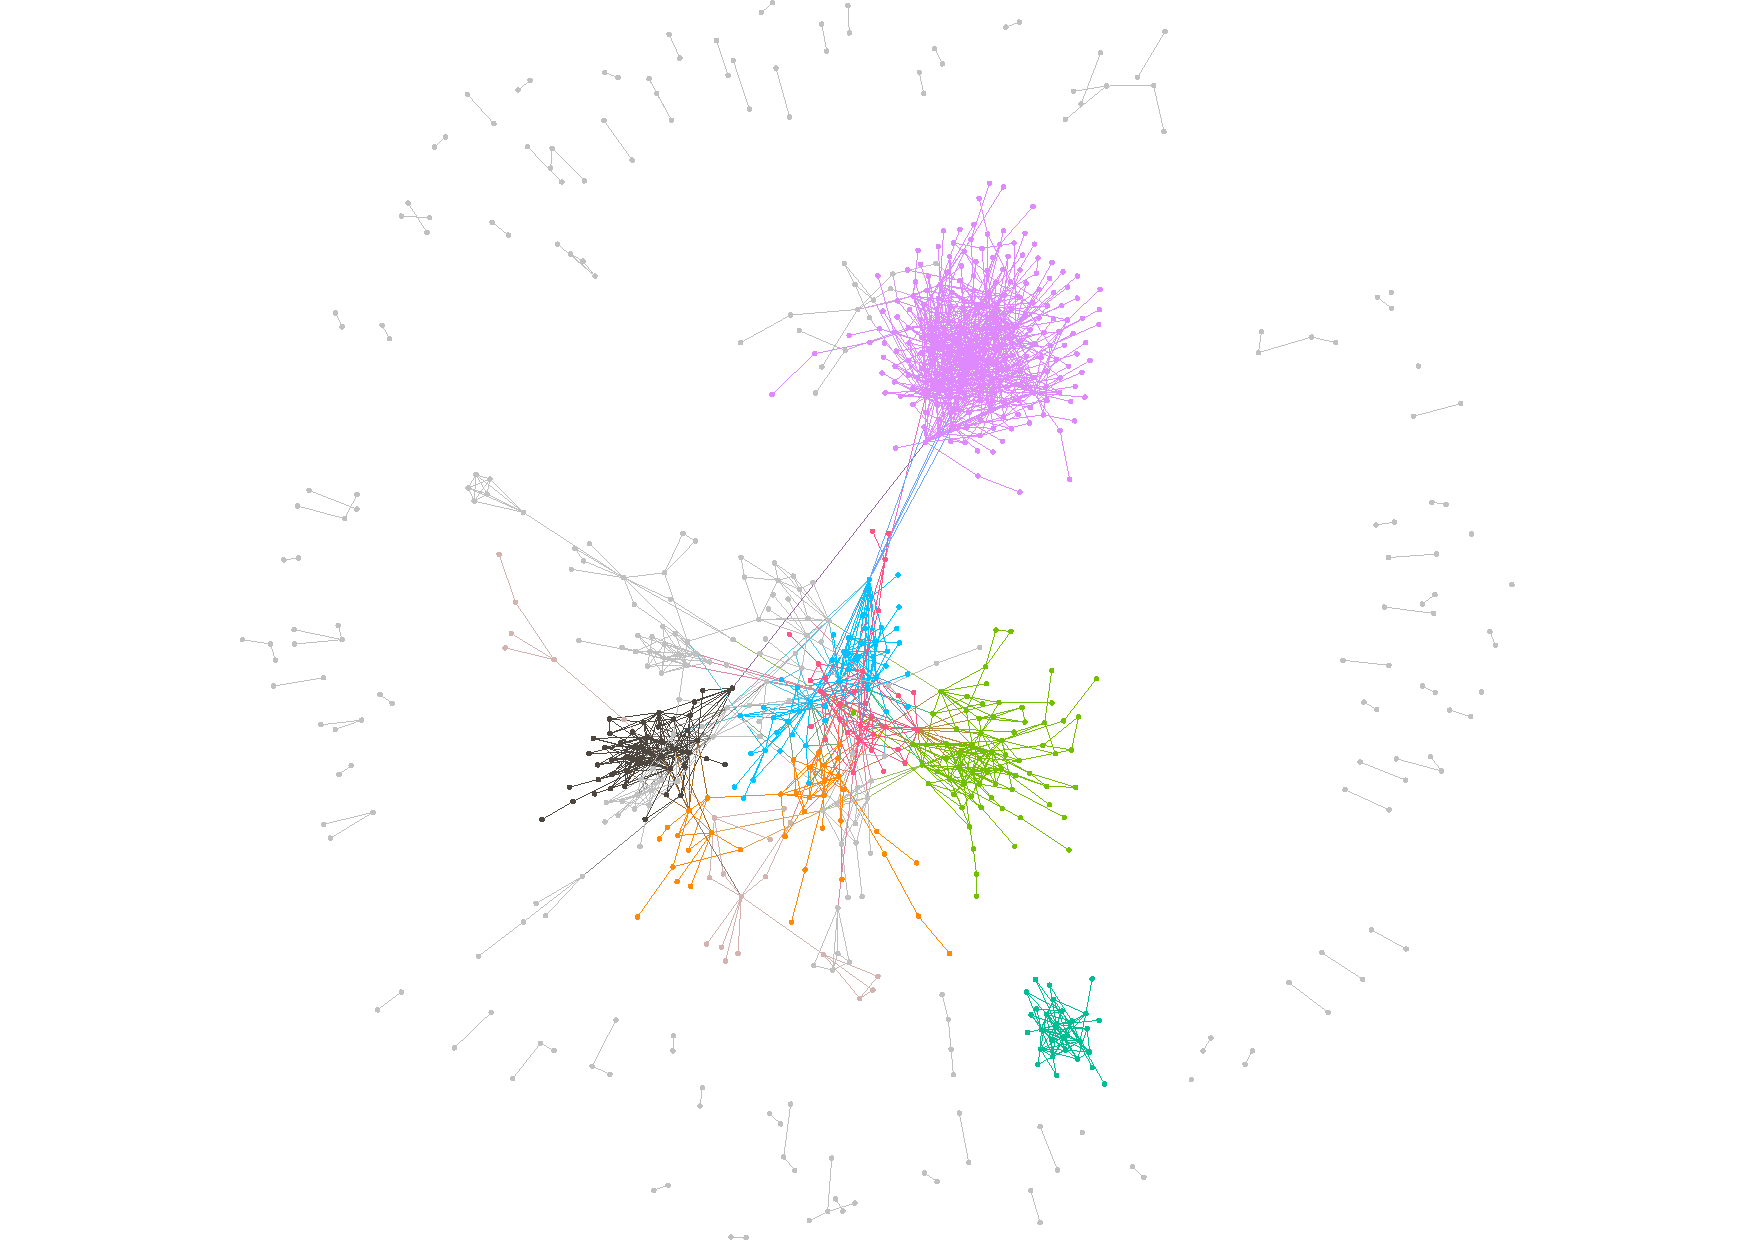
\includegraphics[page=1,scale=0.60]{img/GrafoCollaborazioni.pdf}}
\captionof{figure}{Grafo collaborazioni}
\label{img:grafotutti}
\end{minipage}
}

%\begin{minipage}{1.4\textwidth}
%%[width=\textwidth]
%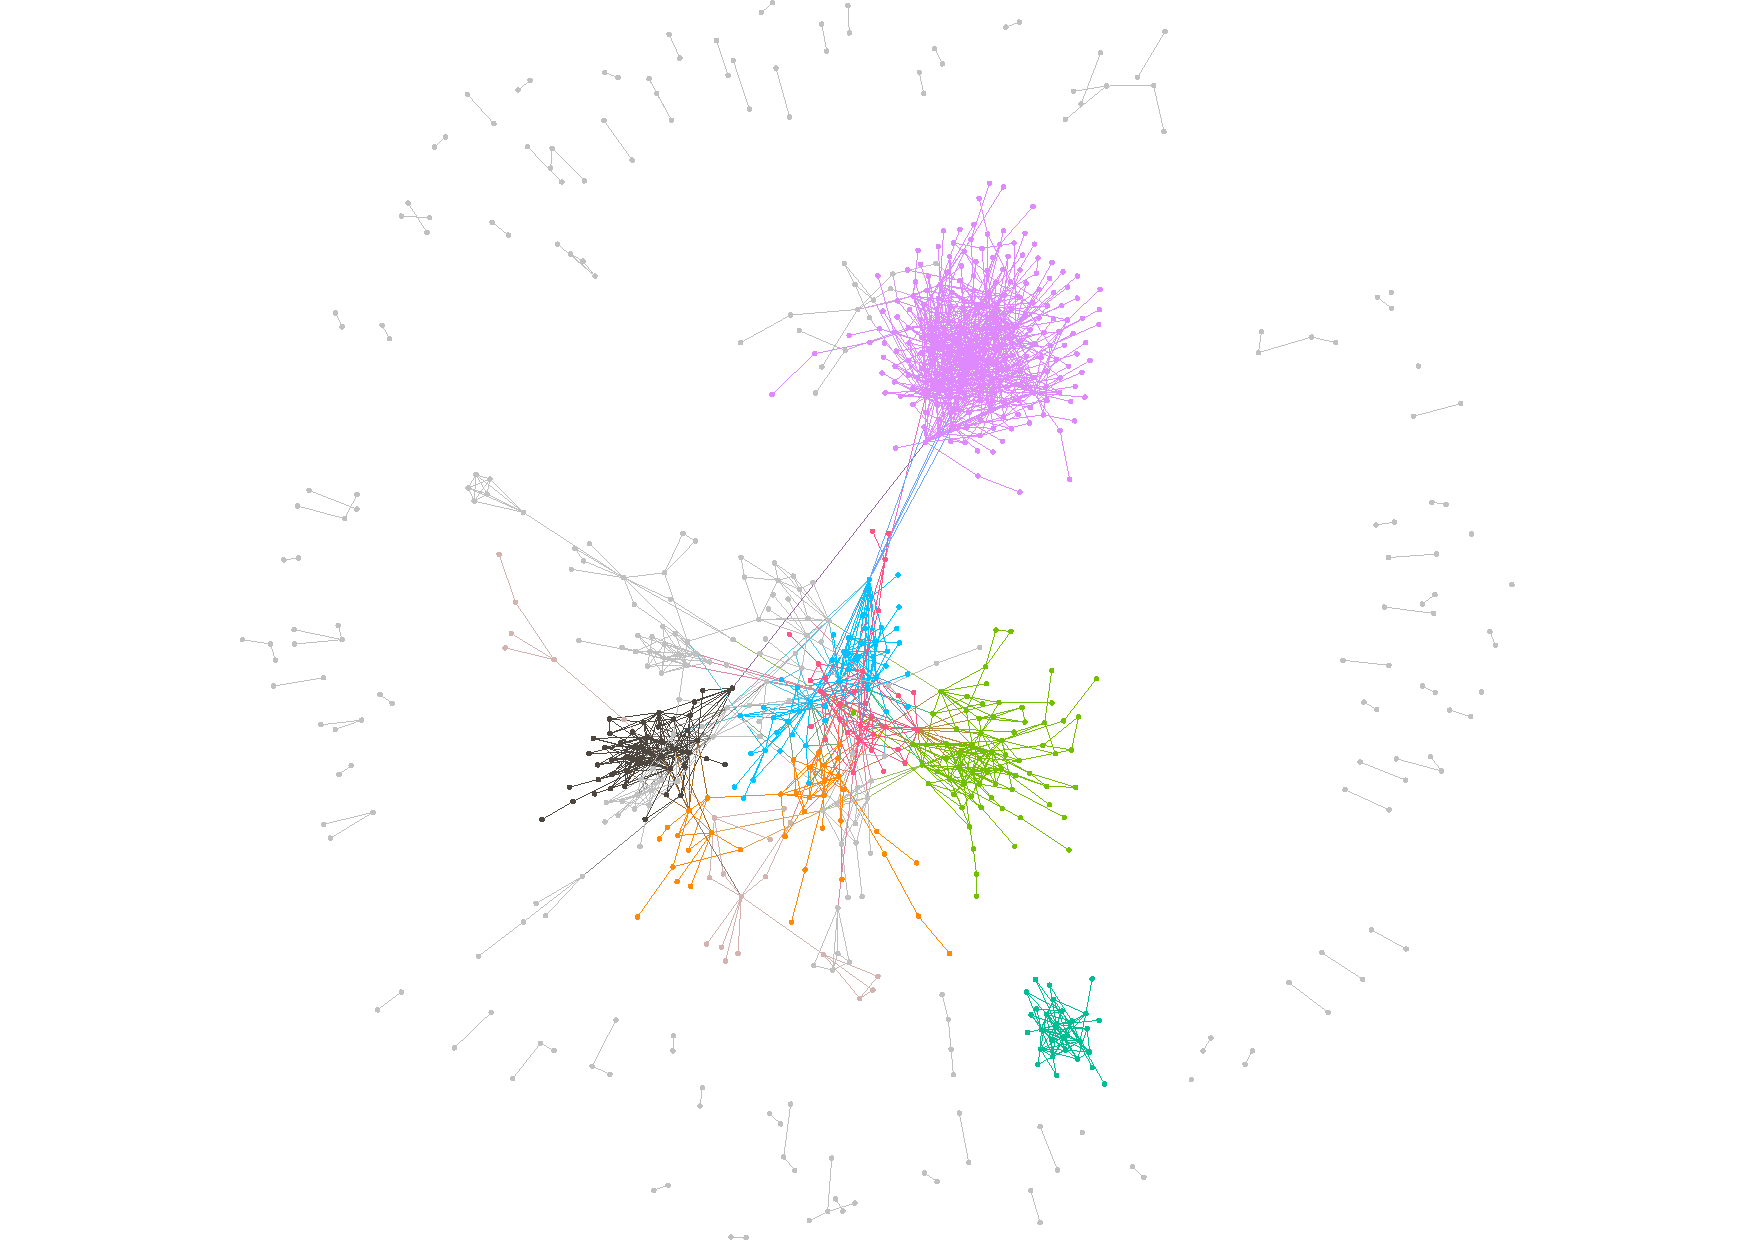
\includepdf{img/GrafoCollaborazioni.pdf}
%\captionof{figure}{Grafo collaborazioni}
%\label{img:grafoprimo}
%\end{minipage}
%\clearpage

\subsubsection{Analisi della prima estrazione}\label{ssc:analisiuno}

I due problemi principali di questo processo emergono al momento dell'estrazione degli ID autore dal
file \textit{Authors.txt}:

\begin{itemize}[noitemsep, topsep=0pt]
\item
Vengono selezionati anche gli ID riferiti ad autori omonimi, non affiliati al DEI.
\item
Ad un singolo autore DEI sono associati più ID autore.
\end{itemize}

%::::PADOVANI::::
\subsection{Filtro degli autori per affiliation} \label{ssc:padovani}
Il primo problema è già in parte risolto dal metodo di creazione del grafo, che considera solo gli
ID autori che hanno almeno una collaborazione con un altro ID nel set. In questo modo più del 90\%
degli ID viene filtrato.

Ispezionando manualmente il grafo, si rileva la presenza di due nodi riferiti a "c pizzi", che però
sono connessi ad autori con cui la professoressa Pizzi non ha mai collaborato. Analizzando gli ID,
le loro collaborazioni e i paper a cui hanno collaborato, si è dedotto che sono ID relativi
probabilmente a Carmine Pizzi e Claudia Pizzi, medici rispettivamente a Bologna e Milano. Questi ID
sono stati inclusi perché risultano collaborazioni con altri autori il cui nome è presente nella
lista di partenza estratta dal sito di dipartimento.

È stato sviluppato un secondo metodo di estrazione dei dati che esclude gli ID autore se non hanno
mai pubblicato un paper a Padova, considerando le informazioni sulle affiliation dei paper, come
viene illustrato di seguito.

\begin{itemize}[noitemsep, topsep=0pt]
\item[--]
Dal file \textit{Affiliations.txt} si estrae la lista delle affiliation in cui risulta nel nome un match all'espressione regolare ``$pad(ov|u)a$''.
% TODO usare un set di affiliation solo di dipartimento (circa 300) è troppo poco
\item[--]
% TODO richiamare la lista di terne
Dalla lista di terne (ID paper, ID autore, ID affiliation) si mantengono solo quelle in cui l'ID affiliation compare nel set di affiliation padovane appena estratte.
\item[--]
Dalle terne selezionate, si estrae un set di ID autori che hanno pubblicato almeno un paper con affiliation padovana.
\item[--] % TODO meglio - più punti
Si estraggono i paper scritti da questi ID autore e si procede alla generazione degli edge pesati.
\end{itemize}

Applicando questo metodo, gli ID autore si riducono a 306, relativi a 201 nomi univoci. Il grafo
generato include 850 edge con un peso totale di 5.195.

Gli ID autore riferiti a "c pizzi", non avendo neanche un paper con affiliation padovana, vengono
correttamente filtrati.

\centerline{
\begin{minipage}{1.10\textwidth}
\setlength{\fboxrule}{0pt}	%barbatrucco per far sparire il bordo della box
\fbox{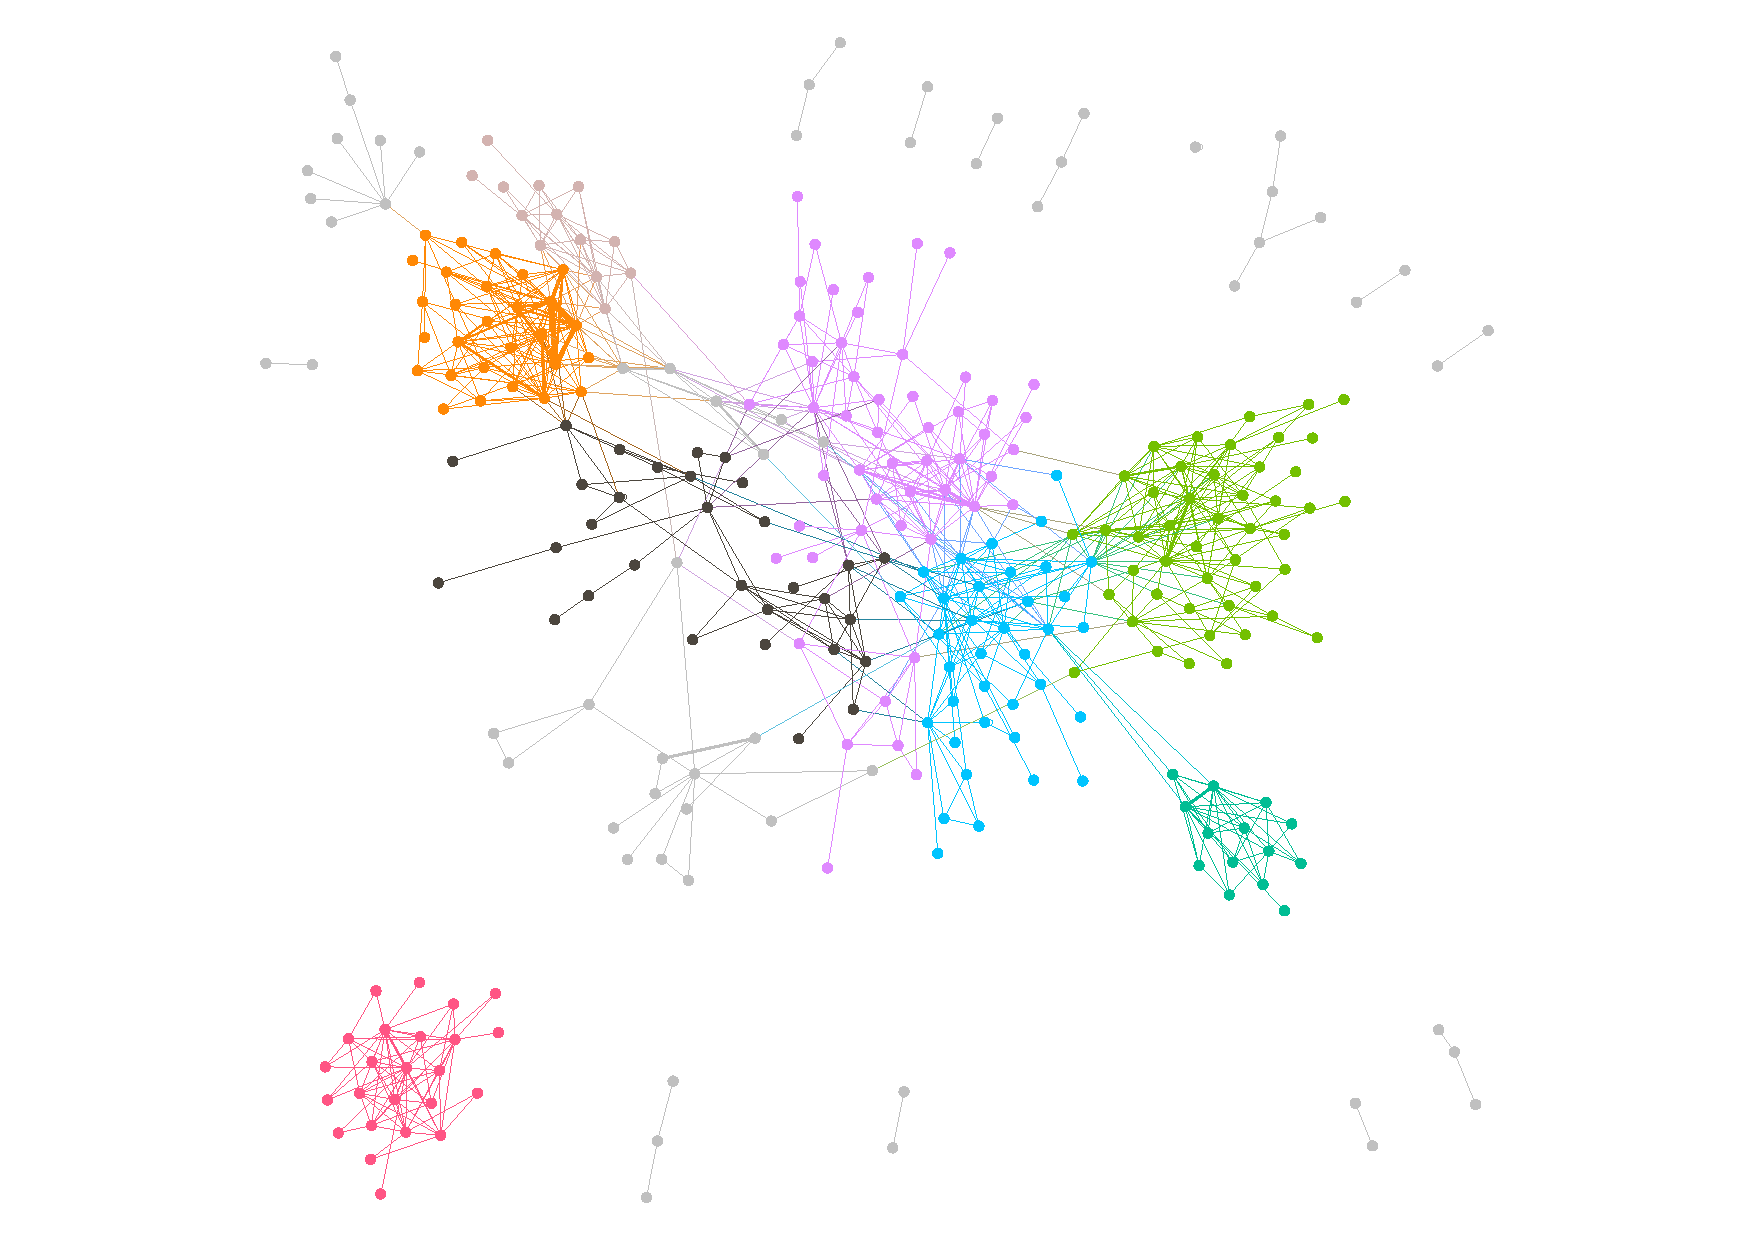
\includegraphics[page=1,scale=0.45]{img/GrafoPadovani.pdf}}
\captionof{figure}{Grafo Padovani}
\label{img:grafopad}
\end{minipage}
}

%::::::::::::::::::::::::::::::::::COLLASSANODI::::::::::::::::::::::::::::::::::::::::::::::::::::::
\subsection{Unione di ID autore in singoli nodi} \label{ssc:collassa}
% TODO esempio di qualcuno
Per risolvere il secondo problema insorto nell'estrazione dei dati, per cui ad una singola persona
fisica, effettivamente affiliata al DEI, possono essere associati più ID autore, sono state seguite
due vie alternative fra loro.

Il primo metodo tiene conto solo dei nomi associati ai nodi del grafo, il secondo metodo sfrutta la
struttura del grafo per stabilire se due nodi siano riferiti alla stessa persona.

% I grafi precedentemente generati vengono rielaborati

\subsubsection{Per nome} \label{ssc:nomi} % questo label è inutile

I grafi precedentemente generati vengono rielaborati, ipotizzando che nodi con nomi uguali o le cui
abbreviazioni sono uguali possano essere considerati un unico nodo.

In questo modo ``\textit{a alberto pietracaprina}'' viene associato a ``\textit{a a
pietracaprina}'' ma anche a ``\textit{andrea a pietracaprina}'' come pure a ``\textit{andrea alberto
pietracaprina}''.

I nodi del grafo in figura \ref{img:grafotutti} si riducono da 778 a 199. Gli edge scendono da 1830
a 661, mantenendo lo stesso peso totale di 7.803.

\centerline{
\begin{minipage}{1.10\textwidth}
\setlength{\fboxrule}{0pt}	%barbatrucco per far sparire il bordo della box
\fbox{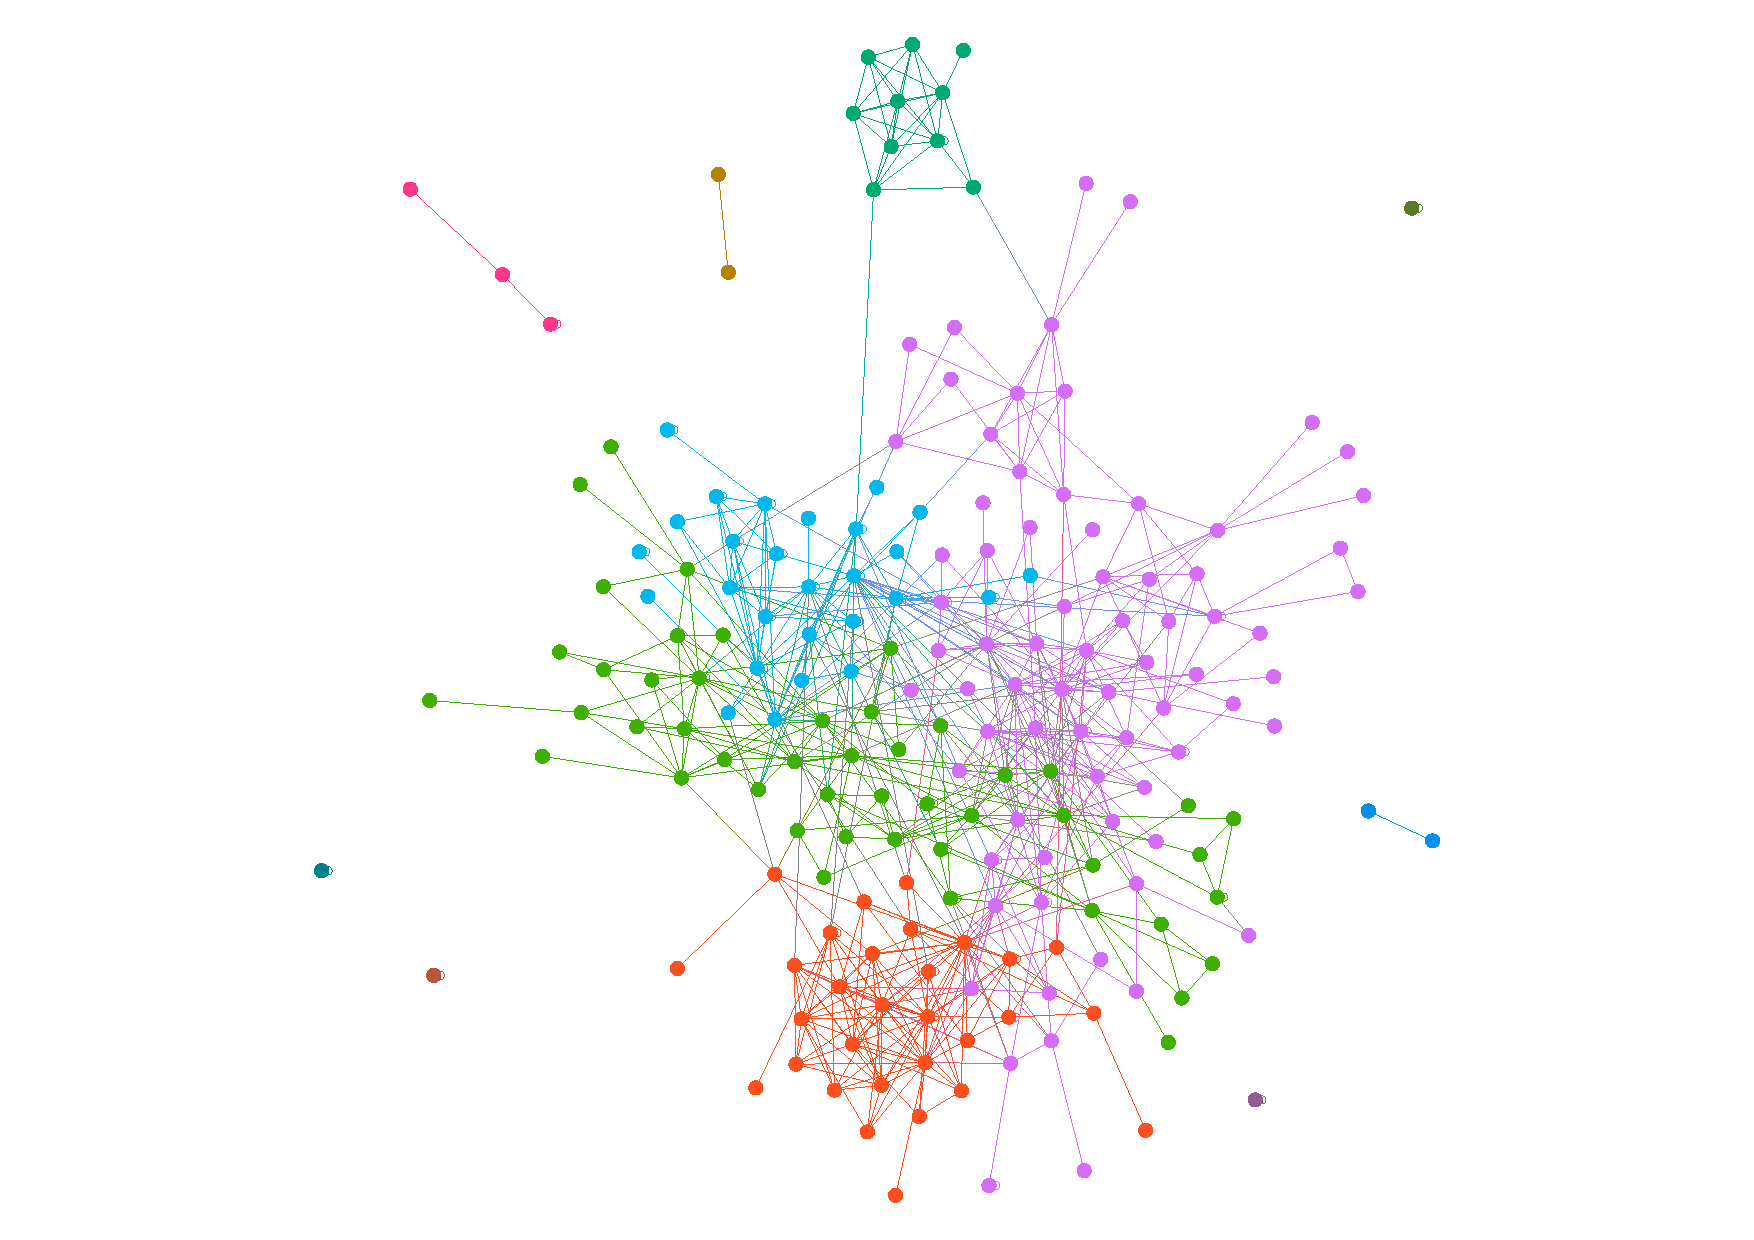
\includegraphics[page=1,scale=0.37]{img/GrafoTuttiNomi.pdf}}
\captionof{figure}{Grafo collaborazioni - nodi unificati per nome}
\label{img:grafotuttinome}
\end{minipage}
}

% \clearpage % grafica da fare alla fine
I nodi del grafo in figura \ref{img:grafopad} si riducono da 306 a 158. Gli edge scendono da 850 a
463, mantenendo il peso totale di 5.195.

\centerline{
\begin{minipage}{1.10\textwidth}
\setlength{\fboxrule}{0pt}	%barbatrucco per far sparire il bordo della box
\fbox{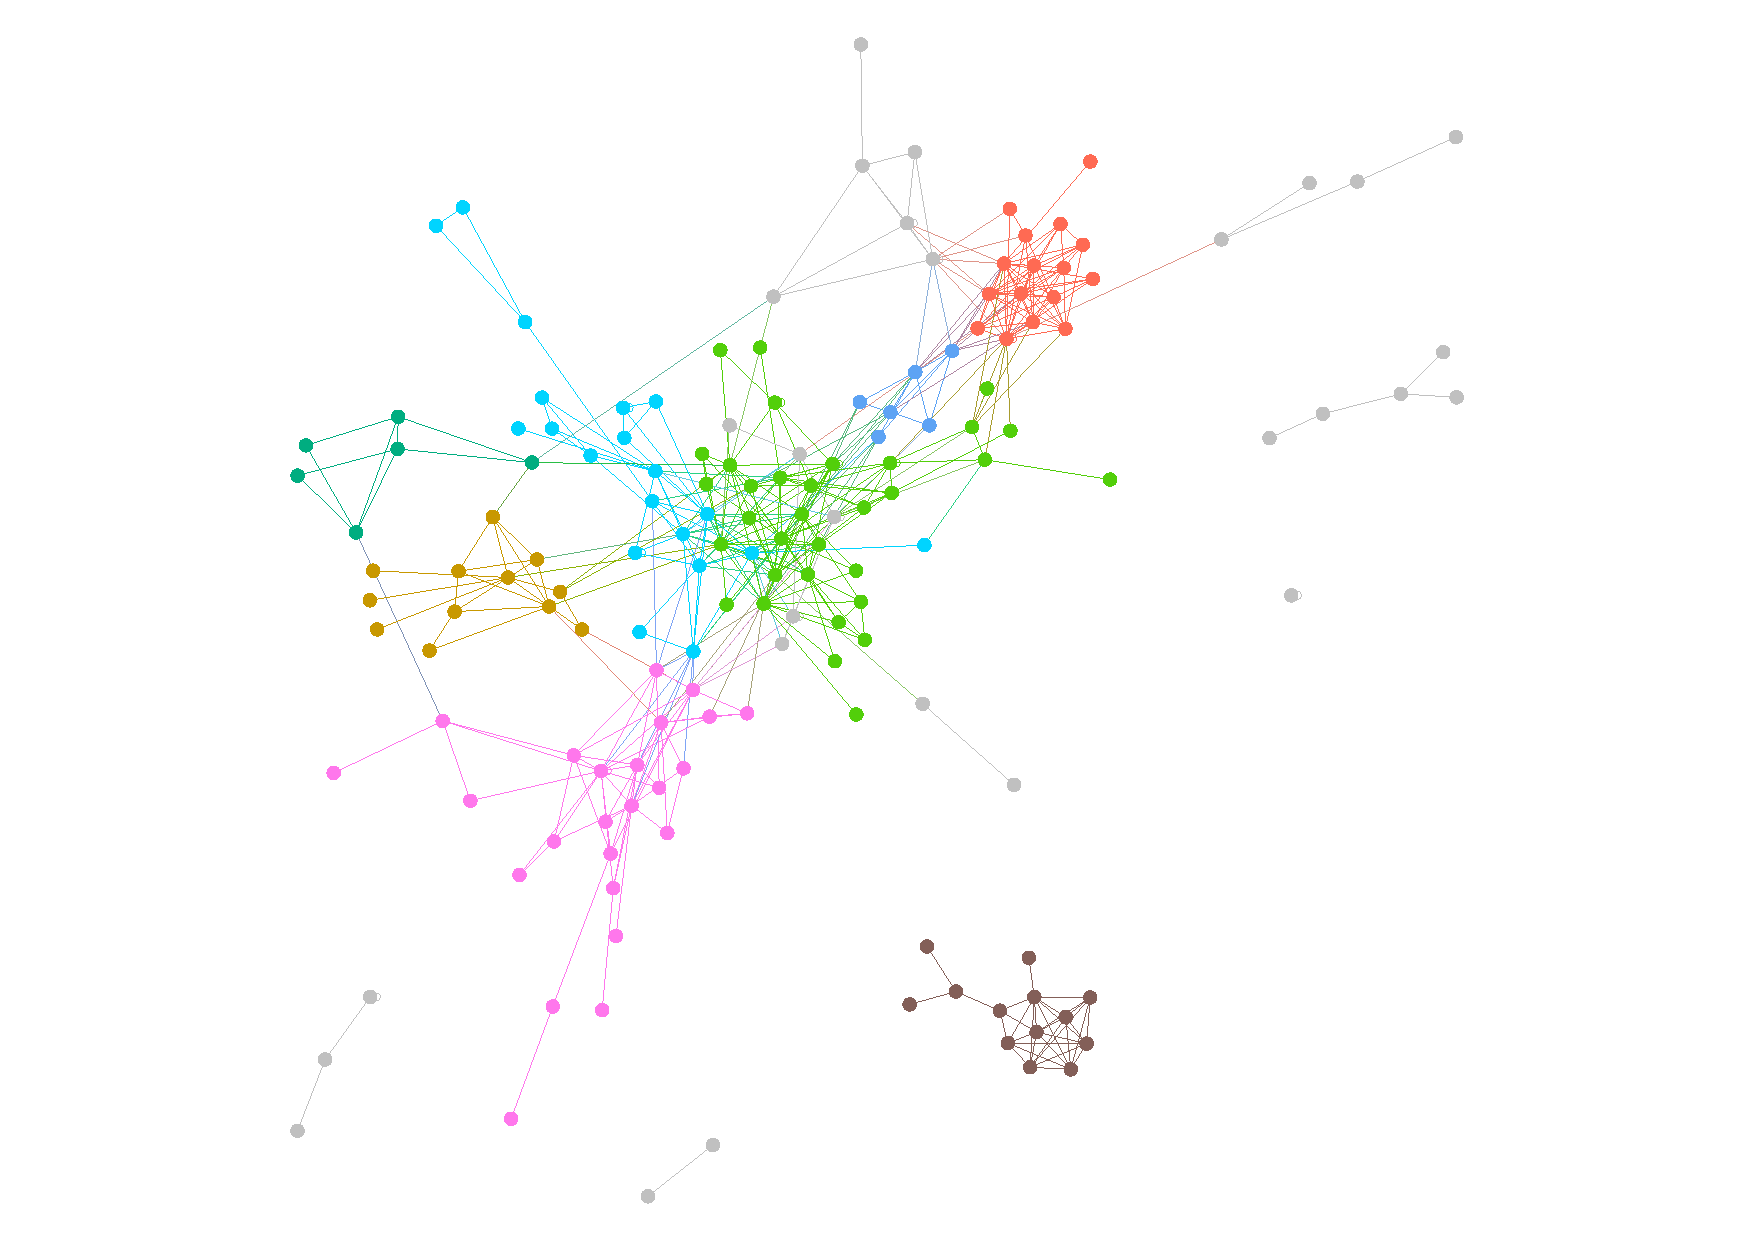
\includegraphics[page=1,scale=0.37]{img/GrafoPadovaniNomi.pdf}}
\captionof{figure}{Grafo padovani - nodi unificati per nome}
\label{img:grafopadnome}
\end{minipage}
}

\subsubsection{Per distanza} \label{ssc:distanza}

Il metodo che considera i nomi precedentemente descritto introduce una criticità nel caso un cui due
autori abbiano un nome che viene abbreviato nello stesso modo.
Questo fa sì che più persone vengano assimilate erroneamente in un unico nodo.

Nei dati che sono stati trattati questo succede solo nel caso di ``\textit{Mattia Zorzi}'' e
``\textit{Michele Zorzi}'', che si abbreviano entrambi in ``\textit{m zorzi}''.

In dataset più ampi oppure relativi a comunità che anche se ristrette presentano una bassa
variabilità dei cognomi, il fenomeno dei falsi positivi incide in maniera molto più marcata sulla
veridicità del grafo.

Nel secondo metodo sviluppato per unificare i nodi, viene richiesta un'ulteriore condizione per
considerare due nodi come relativi alla stessa persona fisica. Oltre a verificare la corrispondenza
delle abbreviazioni dei nomi si calcola anche la distanza minima tra i due nodi nel grafo. Se questa
distanza è minore di una certa soglia, i due nodi vengono unificati. Questo processo può essere
iterato più volte, per sfruttare le informazioni ottenute nei passi precedenti.

% \clearpage % grafica da fare alla fine
\begin{center}
\captionof*{table}{Prima iterazione unione nodi con distanza minima minore di 2}
\begin{minipage}{0.40\textwidth}
\begin{tikzpicture}
\GraphInit[vstyle=Normal]
%\draw[help lines] (0,0) grid (4,3);
\Vertex[L=D]{d1} % par défaut x = 0 et y = 0
\Vertex[x=1 , y=1.5, L=A]{a2}
\Vertex[x=0 , y=3, L=C]{c1}
\Vertex[x=2 , y=0, L=A]{a1}
\Vertex[x=2 , y=3, L=B]{b1}
\Vertex[x=3 , y=1.5, L=A]{a3}
\Vertex[x=4 , y=3, L=C]{c2}
\Edge[label=3](c1)(a2)
\Edge[label=8](a3)(c2)
\SetUpEdge[style={ultra thick},color=red]
\Edge[label=6](d1)(a1)
\Edge[label=7](d1)(a2)
\SetUpEdge[style={ultra thick},color=cyan]
\Edge[label=1](a2)(b1)
\Edge[label=2](b1)(a3)
\end{tikzpicture}
\end{minipage}
\begin{minipage}{0.075\textwidth}
$\rightarrow$
\end{minipage}
\begin{minipage}{0.40\textwidth}
\begin{tikzpicture}
\GraphInit[vstyle=Normal]
\Vertex[L=D]{d1} % par défaut x = 0 et y = 0
\Vertex[x=2 , y=1.5, L=A]{a2}
\Vertex[x=0 , y=3, L=C]{c1}
\Vertex[x=2 , y=3, L=B]{b1}
\Vertex[x=4 , y=3, L=C]{c2}
\Edge[label=13](d1)(a2)
\Edge[label=3](a2)(b1)
\Edge[label=3](c1)(a2)
\Edge[label=8](a2)(c2)
\end{tikzpicture}
\end{minipage}
\end{center}

\begin{center}
\captionof*{table}{Seconda iterazione unione nodi con distanza minima minore di 2}
\begin{minipage}{0.40\textwidth}
\begin{tikzpicture}
\GraphInit[vstyle=Normal]
\Vertex[L=D]{d1} % par défaut x = 0 et y = 0
\Vertex[x=2 , y=1.5, L=A]{a2}
\Vertex[x=0 , y=3, L=C]{c1}
\Vertex[x=2 , y=3, L=B]{b1}
\Vertex[x=4 , y=3, L=C]{c2}
\Edge[label=13](d1)(a2)
\Edge[label=3](a2)(b1)
\SetUpEdge[style={ultra thick},color=orange]
\Edge[label=3](c1)(a2)
\Edge[label=8](a2)(c2)
\end{tikzpicture}
\end{minipage}
\begin{minipage}{0.075\textwidth}
$\rightarrow$
\end{minipage}
\begin{minipage}{0.40\textwidth}
\begin{tikzpicture}
\GraphInit[vstyle=Normal]
\Vertex[L=D]{d1} % par défaut x = 0 et y = 0
\Vertex[x=2 , y=1.5, L=A]{a2}
\Vertex[x=0.8 , y=3, L=C]{c1}
\Vertex[x=3.2 , y=3, L=B]{b1}
\Edge[label=13](d1)(a2)
\Edge[label=11](c1)(a2)
\Edge[label=3](a2)(b1)
\end{tikzpicture}
\end{minipage}
\end{center}

I valori ottimi di soglia e numero di iterazioni sono stati cercati sperimentalmente, ma non è
emersa dai risultati una coppia di valori migliore in maniera rilevante rispetto alle altre.
% TODO riferimento alla spiegazione del perché nel capitolo 4
Ispezionando manualmente il grafo, si è constatato che ID autore riferiti alla stessa persona
risultano generalmente distanti 2. Il procedimento è stato ripetuto tre volte, in modo da sfruttare
le informazioni generate nei passi predecenti. Dopo questo numero di iterazioni il grafo raggiunge
quasi una situazione di stabilità.

\clearpage % grafica da fare alla fine

I nodi del grafo in figura \ref{img:grafotutti} si riducono da 778 a 336. Gli edge scendono da 1830
a 634, mantenendo lo stesso peso totale di 7.803.

\centerline{
\begin{minipage}{1.20\textwidth}
\setlength{\fboxrule}{0pt}	%barbatrucco per far sparire il bordo della box
\fbox{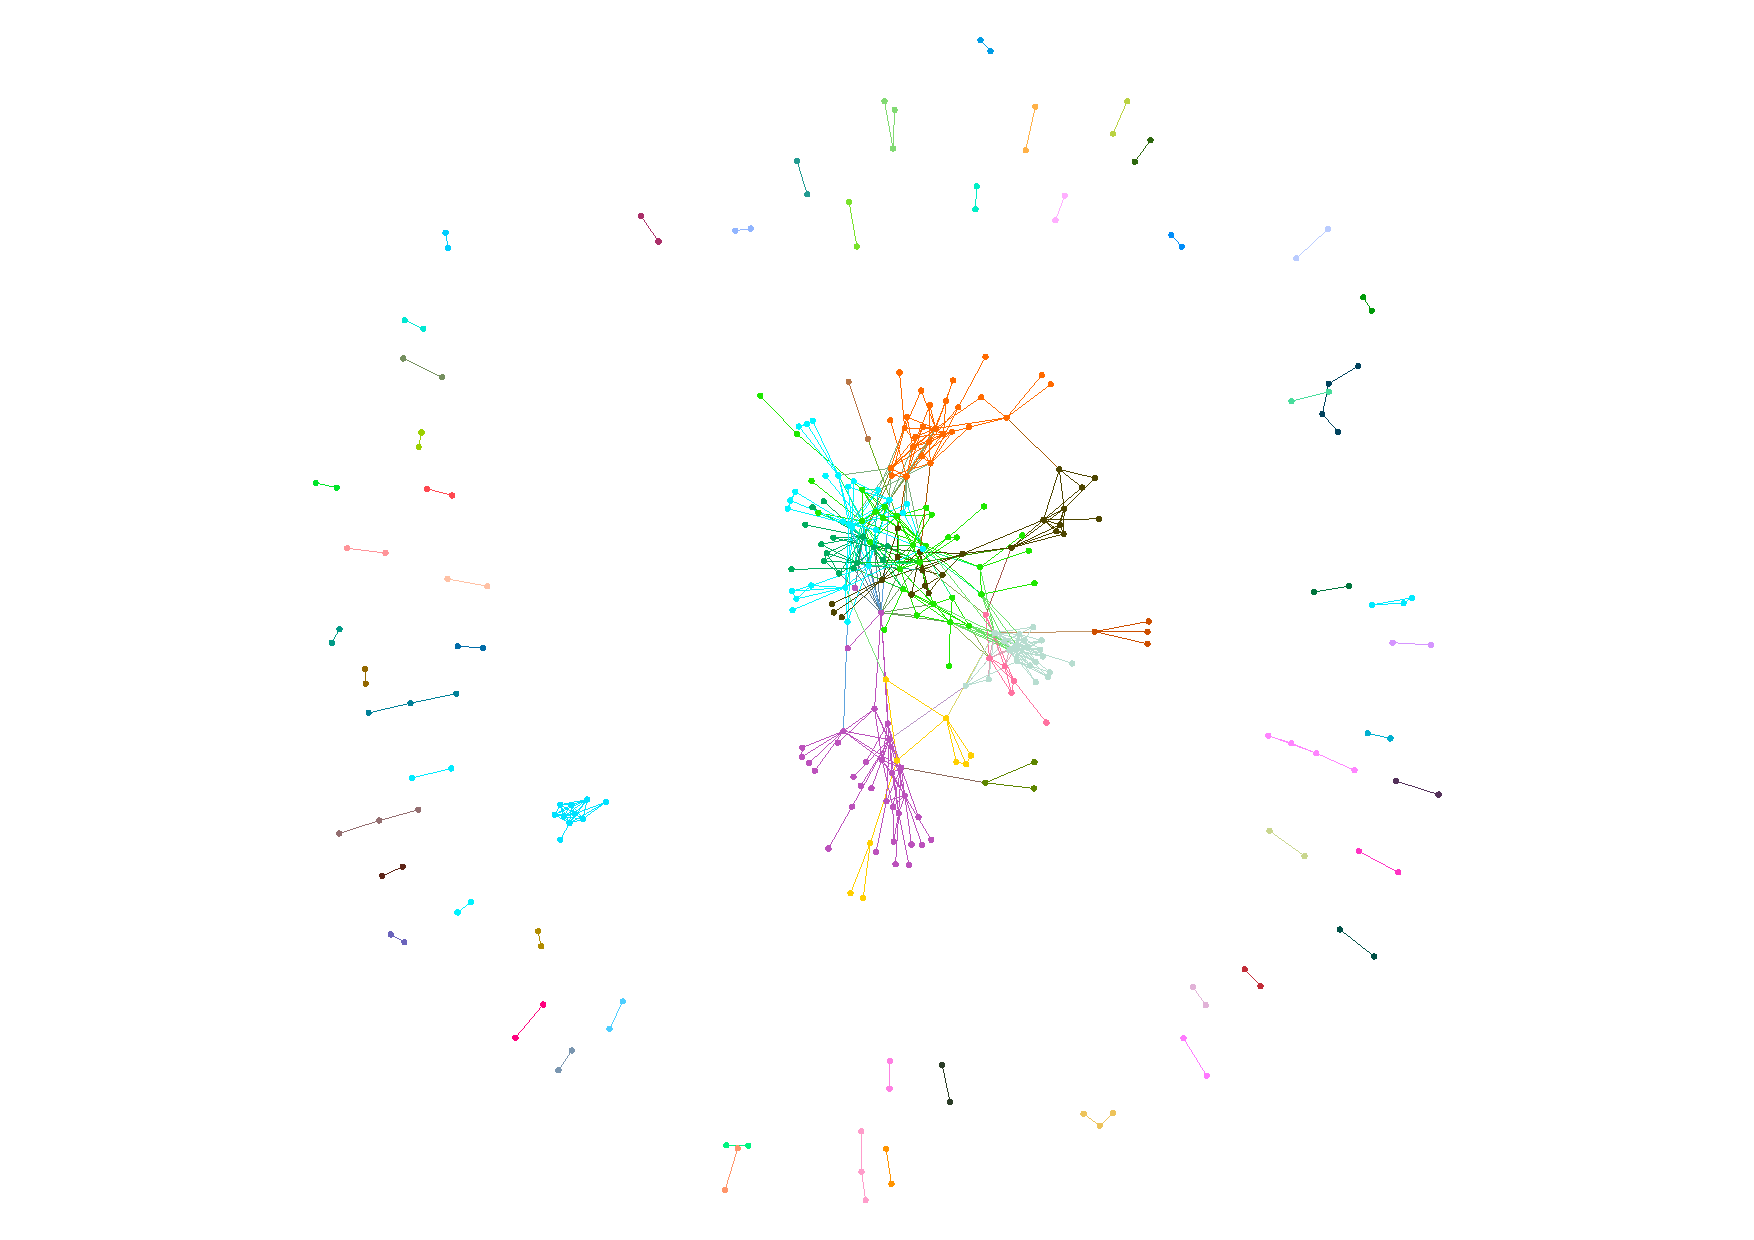
\includegraphics[page=1,scale=0.47]{img/GrafoTuttiDistanza23.pdf}}
\captionof{figure}{Grafo collaborazioni unificati per distanza}
\label{img:grafotuttidistanza}
\end{minipage}
}

I nodi del grafo in figura \ref{img:grafopad} si riducono da 306 a 173. Gli edge scendono da 850 a
439, mantenendo il peso totale di 5.195.

\centerline{
\begin{minipage}{1.00\textwidth}
\setlength{\fboxrule}{0pt}	%barbatrucco per far sparire il bordo della box
\fbox{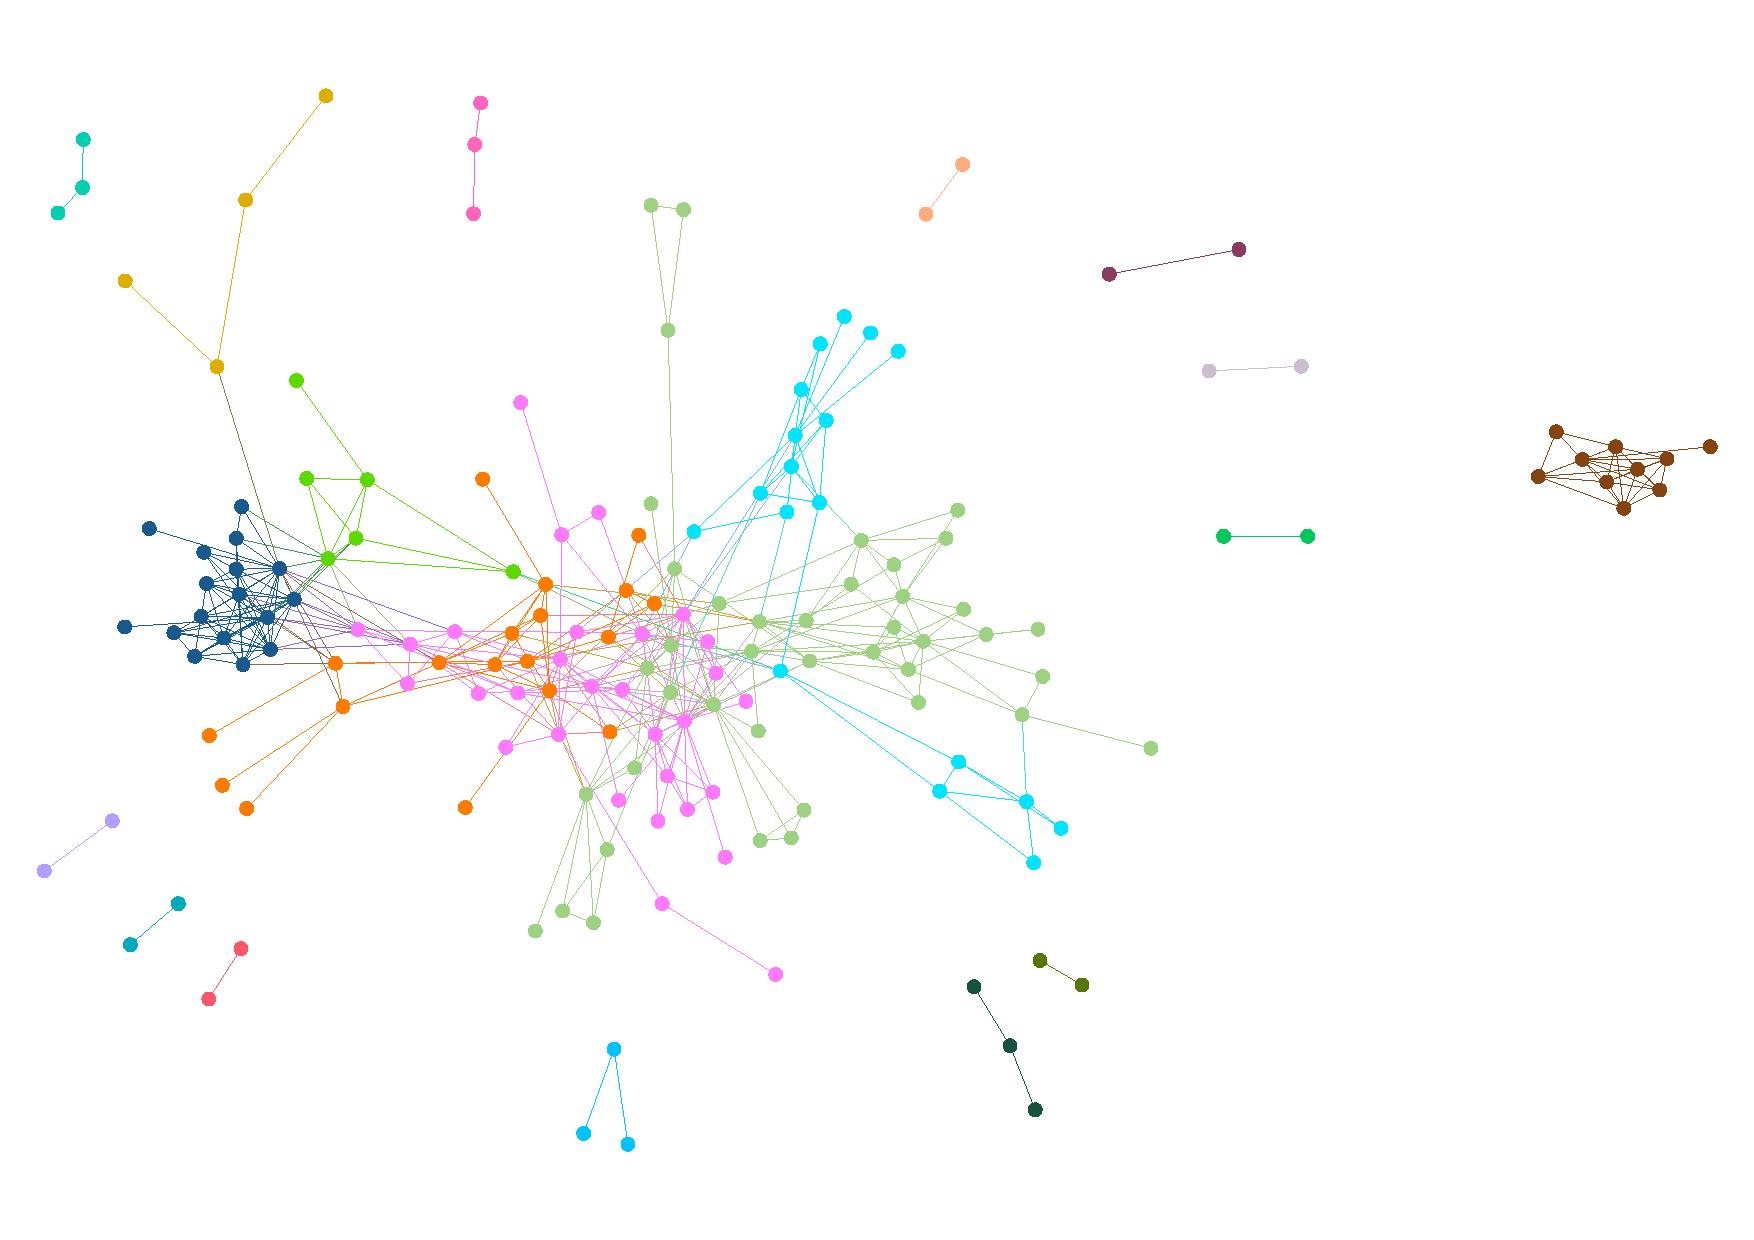
\includegraphics[page=1,scale=0.37]{img/GrafoPadovaniDistanza23.pdf}}
\captionof{figure}{Grafo Padovani unificati per distanza}
\label{img:grafopaddistanza}
\end{minipage}
}

% TODO mostra tabella o grafico dei confronti delle iterazioni varie

\clearpage % grafica da fare alla fine

\subsubsection{Per nodi adiacenti} \label{ssc:edge}
Osservando i grafi generati senza unire i nodi, si nota la presenza di un elevato numero di
componenti sconnesse formate da 2-4 autori, che sono principalmente effettivi collaboratori tra
loro. È stato sviluppato un metodo di deduplicazione dei nodi che si basa sulle collaborazioni tra
coppie di autori.

Per ogni edge si estraggono i nomi relativi agli estremi, se due edge hanno gli estremi con i nomi
coincidenti, si considerano le coppie di nodi come relative alla stessa persona.

\begin{center}
\captionof*{table}{Unione dei nodi per coppie di nodi adiacenti}
\begin{minipage}{0.40\textwidth}
\begin{tikzpicture}
\GraphInit[vstyle=Normal]
\Vertex[L=B]{b1} % par défaut x = 0 et y = 0
\Vertex[x=2 , y=1.5, L=A]{a2}
\Vertex[x=0.5 , y=1.5, L=A]{a1}
\Vertex[x=2.5 , y=3, L=C]{c1}
\Vertex[x=1.5 , y=0, L=B]{b2}
\Vertex[x=4 , y=3, L=C]{c2}
\Edge[label=2](b2)(a2)
\Edge[label=3](a1)(b1)
\Edge[label=4](c1)(a2)
\Edge[label=6](a2)(c2)
\SetUpEdge[style={dashed},color=orange]
\Edge(b1)(b2)
\Edge(a1)(a2)
\Edge(c1)(c2)
\end{tikzpicture}
\end{minipage}
\begin{minipage}{0.075\textwidth}
$\rightarrow$
\end{minipage}
\begin{minipage}{0.40\textwidth}
\begin{tikzpicture}
\GraphInit[vstyle=Normal]
\Vertex[L=B]{b1} % par défaut x = 0 et y = 0
\Vertex[x=2 , y=1.5, L=A]{a2}
\Vertex[x=4 , y=3, L=C]{c1}
\Edge[label=10](c1)(a2)
\Edge[label=5](a2)(b1)
\end{tikzpicture}
\end{minipage}
\end{center}

I nodi del grafo in figura \ref{img:grafotutti} si riducono da 778 a 313. Gli edge scendono da 1830
a 615, mantenendo lo stesso peso totale di 7.803.

\centerline{
\begin{minipage}{1.05\textwidth}
\setlength{\fboxrule}{0pt}	%barbatrucco per far sparire il bordo della box
\fbox{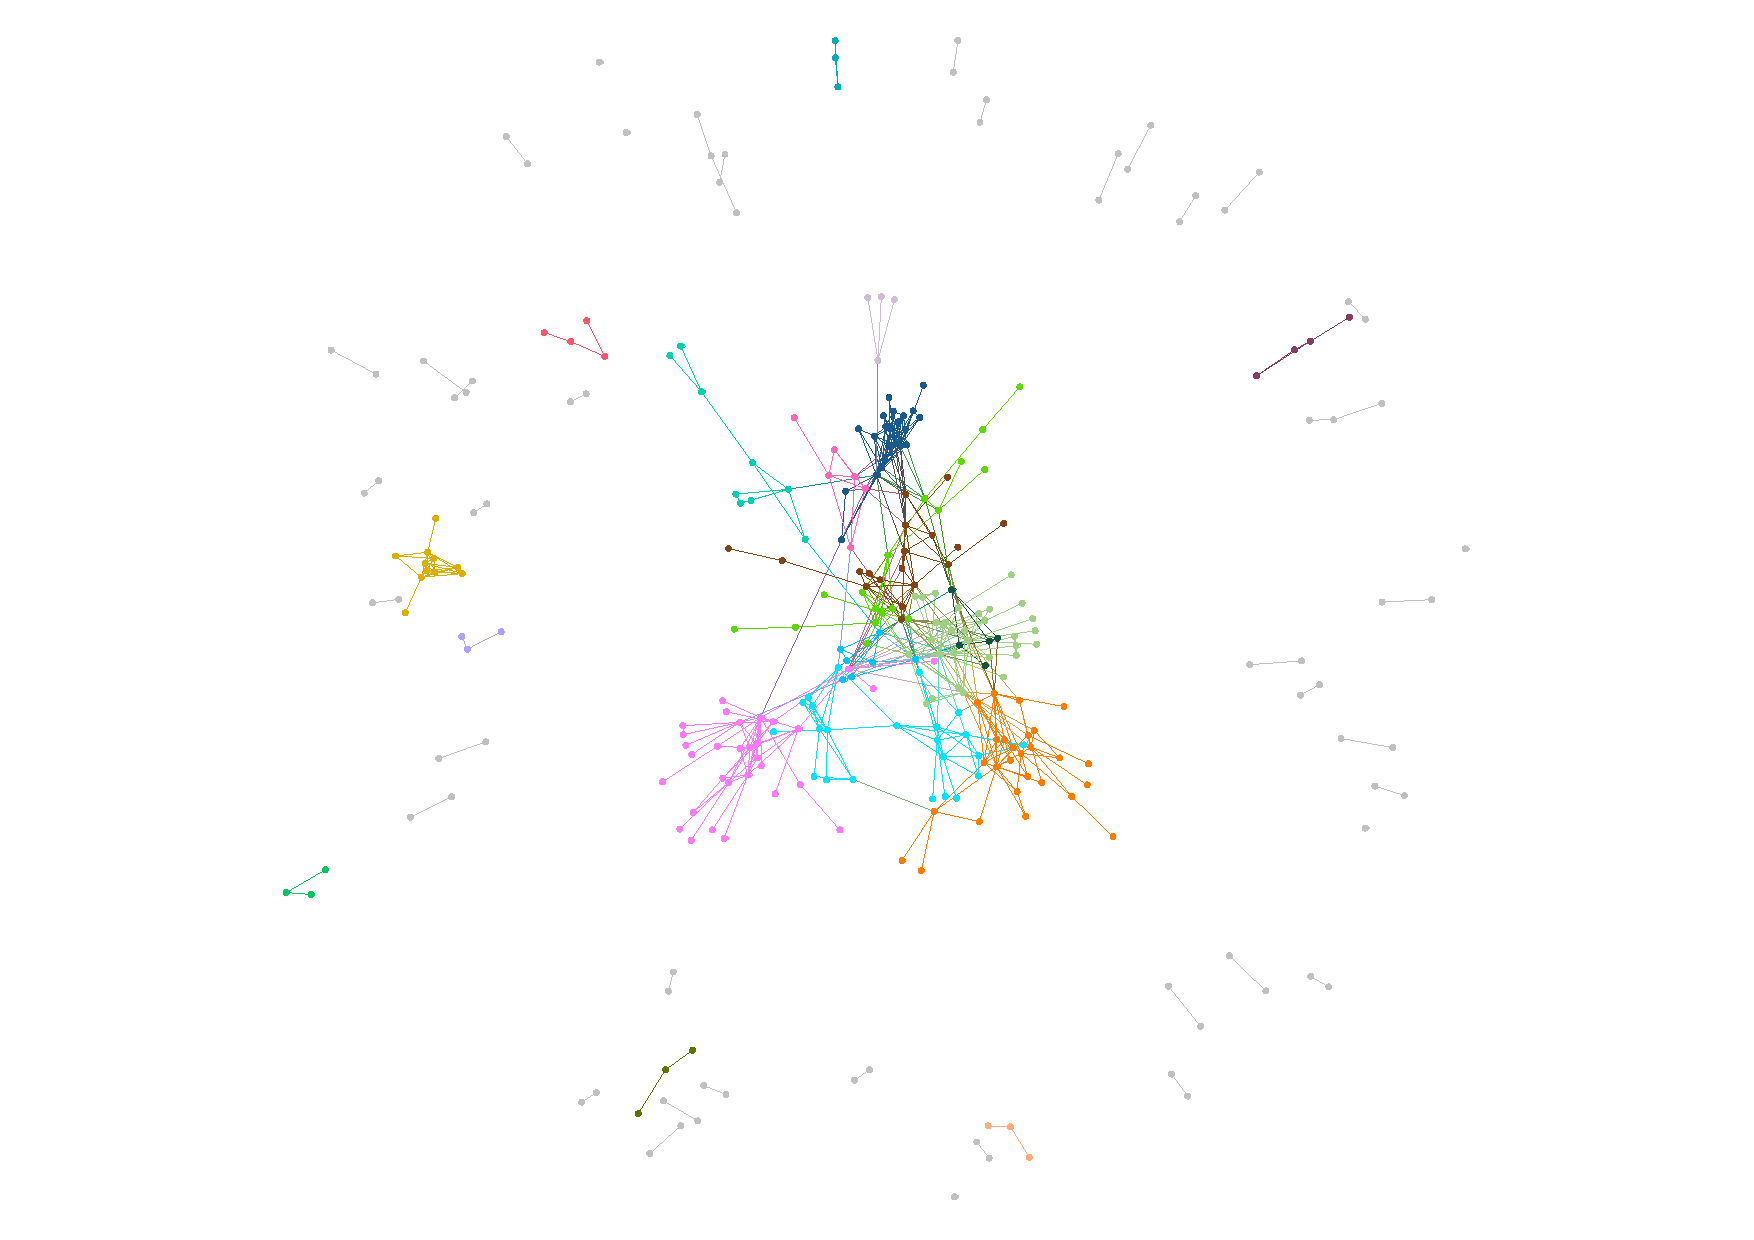
\includegraphics[page=1,scale=0.43]{img/GrafoTuttiEdge.pdf}}
\captionof{figure}{Grafo collaborazioni unificati per coppie di nodi adiacenti}
\label{img:grafotuttiedge}
\end{minipage}
}

\clearpage % grafica da fare alla fine

I nodi del grafo in figura \ref{img:grafopad} si riducono da 306 a 174. Gli edge scendono da 850 a
453, mantenendo il peso totale di 5.195.

\centerline{
\begin{minipage}{1.05\textwidth}
\setlength{\fboxrule}{0pt}	%barbatrucco per far sparire il bordo della box
\fbox{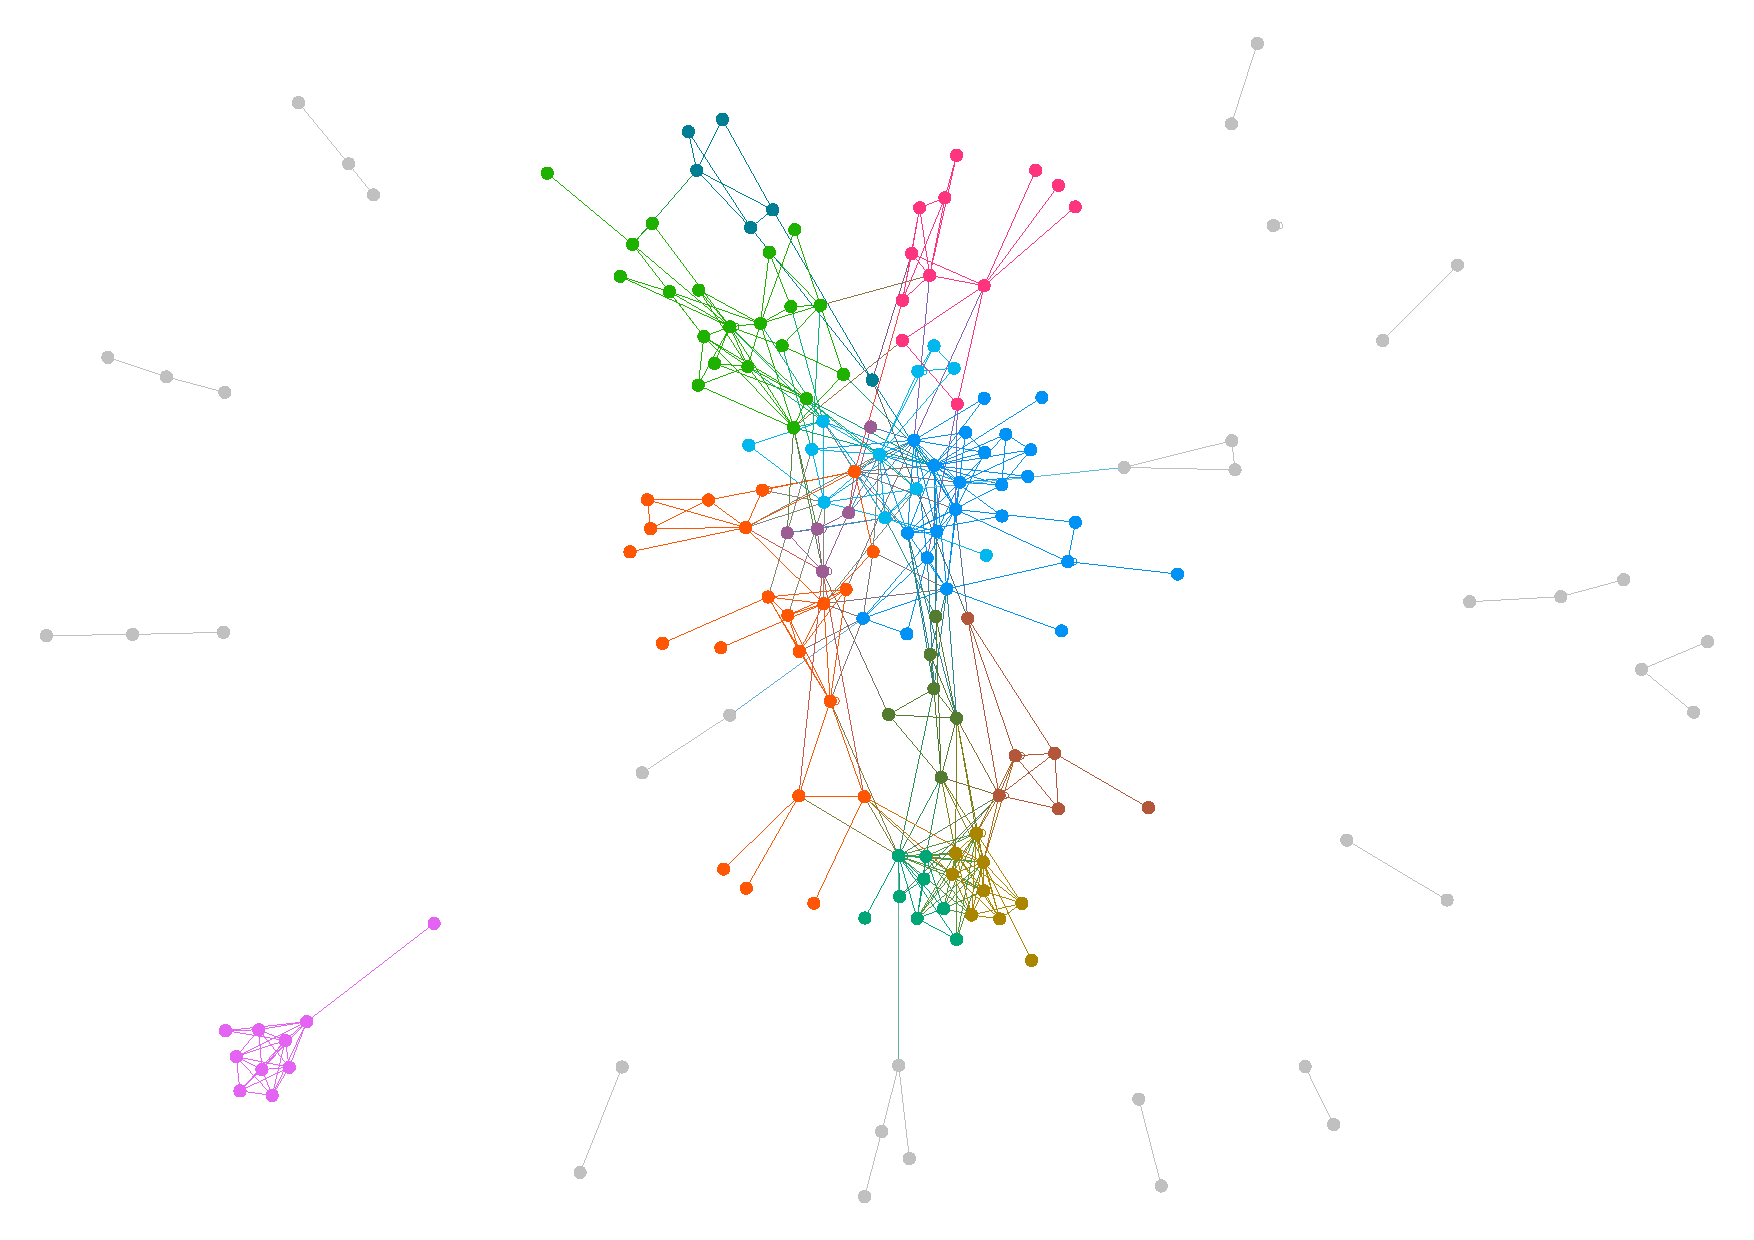
\includegraphics[page=1,scale=0.43]{img/GrafoPadovaniEdge.pdf}}
\captionof{figure}{Grafo Padovani unificati per coppie di nodi adiacenti}
\label{img:grafopadedge}
\end{minipage}
}

\subsection{Errori intrinseci al database} \label{ssc:intrinseci}

Nel corso delle varie iterazioni dell'estrazione dei dati, sono state identificate
varie lacune nei record del database, riassunte di seguito

\begin{itemize}
\item[--]

I record di Paper-Autore-Affiliation non contengono l'ID affiliation in 264.069.014 record su
325.498.062. In particolare per autori con pochi paper, la fase di pruning basata sulle
affiliation è molto influenzata da questa mancanza.

\item[--]

Nei record Paper-Autore-Affiliation, può mancare il record relativo a uno dei coautori.

\item[--]

Tra i coautori dei un paper, possono essere riportati più ID autore riferiti alla stessa persona.

\item[--]

I nomi con caratteri non ASCII sono trattati in maniera imprevedibile.

\end{itemize}

Nel prossimo capitolo si propongono dei metodi alternativi di estrazione dei dati per tentare di
aggirare questi problemi.


\whitePage
\chapter{Troubleshooting} \label{cap:trouble}
Il grafo generato attraverso gli accorgimenti discussi in precedenza presenta ancora delle carenze.

% subsubsection nomi mancanti

In particolare, la lista di partenza include solo gli attuali afferenti DEI, estratti dal sito di
dipartimento. Questo comporta la mancanza di professori, non più attivi a Padova, che avevano ruolo
di aggregatore di una comunità.

Inserendo manualmente Alberto Apostolico, prolifico autore di paper all'Università di Padova, nella
lista di partenza, il grafo, in prossimità del professore, cambia in maniera rilevante, come
illustrato in figura \ref{img:apostolico}. Utilizzando questa procedura, emerge una comunità di
collaboratori che precendentemente erano distanti nel grafo.

\centerline{
\begin{minipage}{0.80\textwidth}
\setlength{\fboxrule}{0pt}	%barbatrucco per far sparire il bordo della box
\fbox{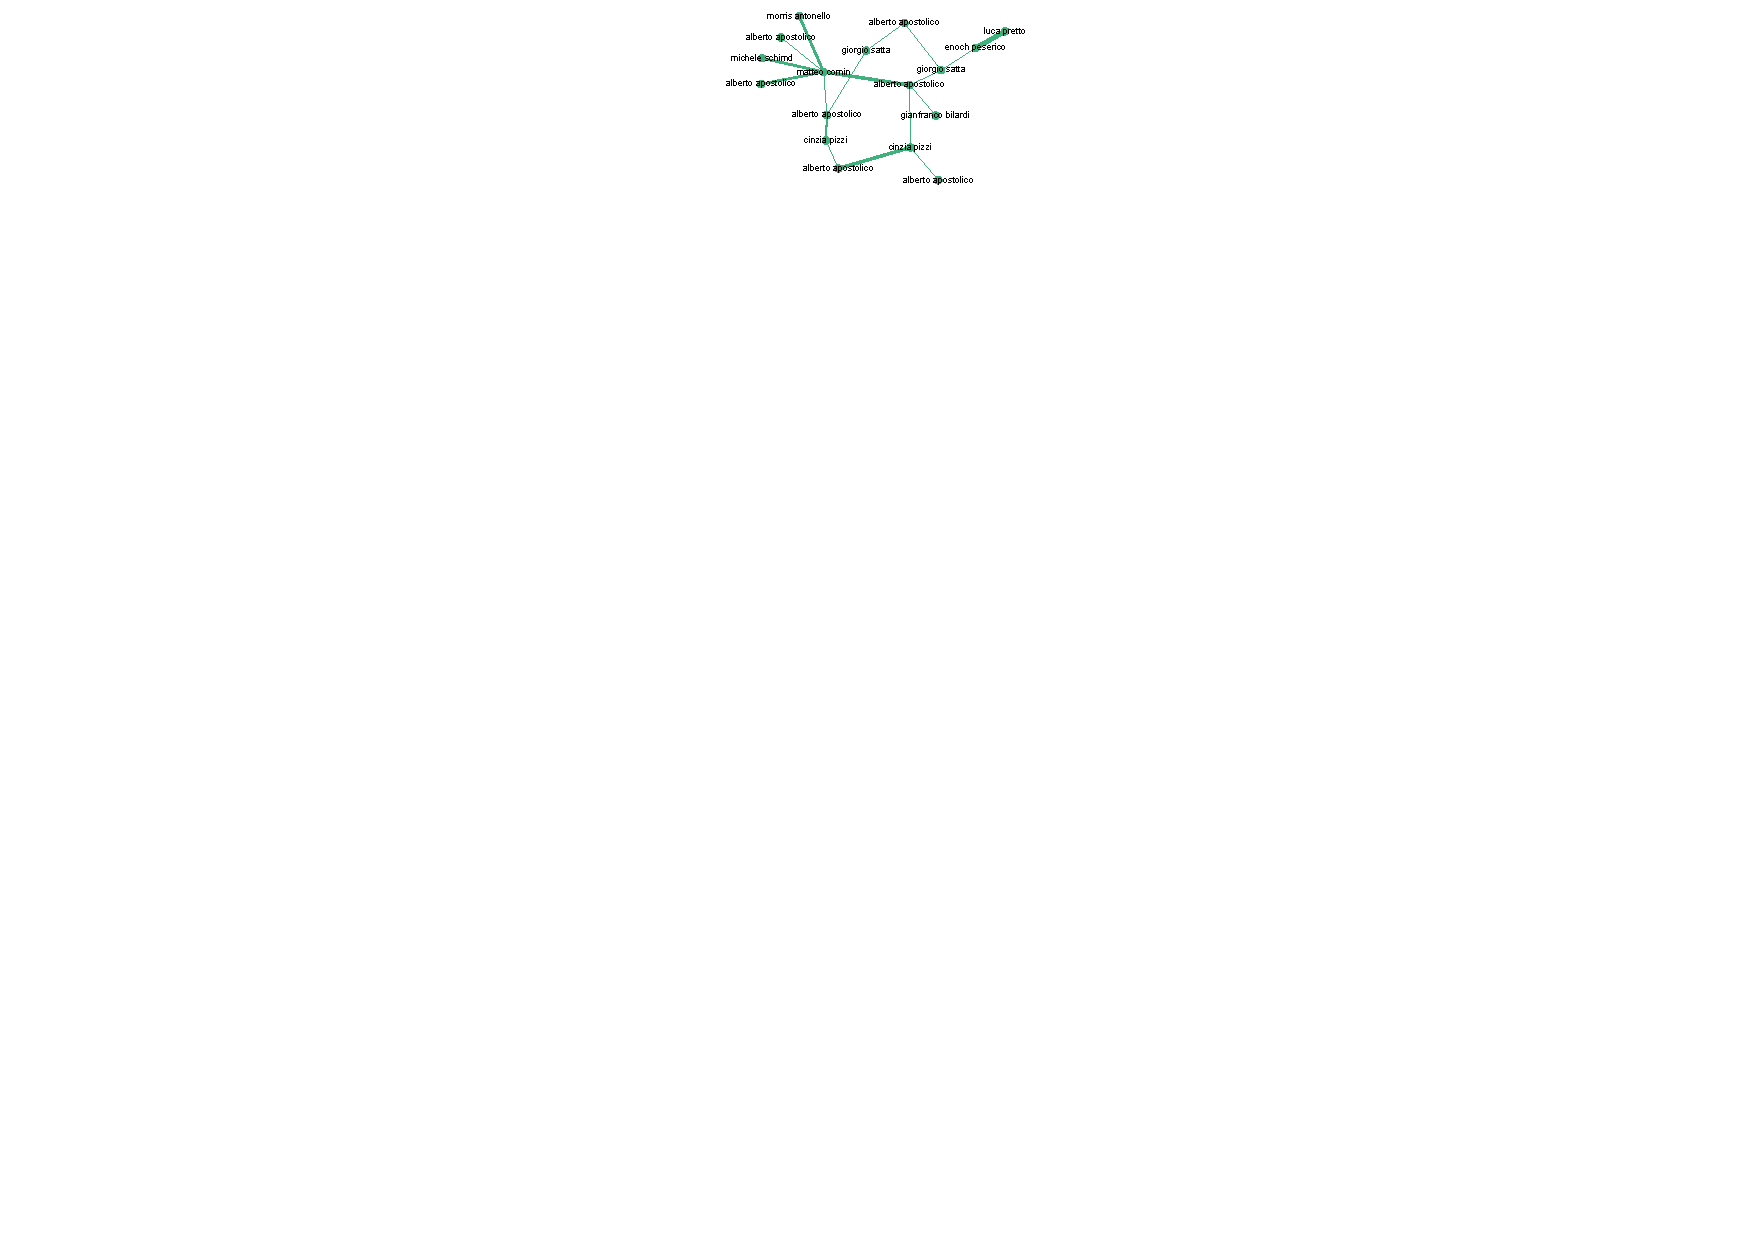
\includegraphics[page=1,scale=1.80]{img/cropped_GrafoApostolico.pdf}}
\captionof{figure}{Rete di collaborazioni del professor Apostolico}
\label{img:apostolico}
\end{minipage}
}

Un metodo generale proposto per identificare anche autori non presenti nella lista degli attuali
afferenti DEI è:

\begin{enumerate}[noitemsep, topsep=0pt]
\item
Estrarre gli ID autore dalla lista di partenza
\item
Estrarre le terne di ID paper-autore-affiliation
\item
Estrarre tutti i record paper-autore-affiliation relativi ai paper identificati al punto precedente
\item
Estrarre una nuova lista di ID autore dai paper appena estratti, ossia i coautori degli autori nella
lista utilizzata al punto 2 per estrarre le terne
\item
Eventualmente ridurre il set di autori basandosi sulle affiliation dei loro paper
\item
Ripetere i passi 2-5 per un numero predefinito di volte o fino alla convergenza della rete, nel
momento in cui non vengono identificati ulteriori coautori
\end{enumerate}

In questo modo si estraggono tutte le comunità relative alle affiliation usate come filtro. Una
singola collaborazione con un dipartimento esterno comporta alle iterazioni successive l'inclusione
di molti autori di quel dipartimento. Un metodo proposto per risolvere il problema e generare una
rete di autori relativa solo al dipartimento di interesse è, alla fine delle iterazioni e della
creazione dei cluster, considerare solo quelli che contengono almeno un nome presente nella lista
originale: in questo modo dipartimenti esterni, anche se connessi al grafo, vengono filtrati.

Gli step 2,3 e 4 sono stati implementati, estraendo 3.845.835 record Paper-Autore-Affiliation,
relativi a 56.450 paper univoci, da cui si ricavano 256.917 ID autore e 193.396 nomi univoci. Questi
valori decisamente elevati di coautori e paper è dovuto alla presenza di riviste, classificate come
paper nel database, a cui hanno collaborato centinaia e anche migliaia di autori.

Filtrando i paper con più di 30 collaborazioni, il set di paper si riduce a 52.001 univoci, su
311.816 record Paper-Autore-Affiliation. Vengono identificati 148.124 ID autore per un totale di
112.440 nomi univoci.

9572 paper univoci padovani
23.417 paper padovani
2.442 ID autori padovani
2.094 nomi univoci



\whitePage
\chapter{Risultati} \label{cap:risultati}

\section{V-measure} \label{sec:vmeasure}

La \textit{V-measure}, una misura esterna della validità
dei cluster basata sull'entropia, presentata da Rosenberg e Hirschberg~\cite{vmeasure}, è stata
utilizzata per valutare la qualità delle partizioni dei grafi ricavati con i vari metodi descritti
nelle sezioni precedenti.

%Per valutare la qualità delle partizioni dei grafi ricavati con i vari metodi descritti nelle
%sezioni precedenti, è stata utilizzata la \textit{V-measure}, come presentata da Rosenberg e
%Hirschberg \cite{vmeasure}, una misura esterna della validità dei cluster basata sull'entropia.

Come terminologia, si parlerà di due distinte partizioni del set di nodi da analizzare: un set di
classi $C$, considerate la suddivisione reale dei nodi, e un set di cluster $K$ per indicare la
partizione generata.

Rosenberg e Hirschberg hanno sviluppato due concetti, l'omogeneità e la completezza, la cui media
armonica è la V-measure.

Una partizione di cluster è considerata perfettamente omogenea quando i cluster contengono
\textit{solo} membri di una singola classe.

In maniera simmetrica una partizione è perfettamente completa quando un singolo cluster contiene
\textit{tutti} i membri di una classe.

Per valutare l'omogeneità di una partizione si considera l'entropia condizionata della distribuzione
di classi dato il clustering generato $H(C|K)$. Nel caso di perfetta omogeneità questo valore è
nullo in quanto il cluster contiene una singola classe, mentre è massimo e vale $H(C)$ quando la
distribuzione delle classi all'interno del cluster è identica alla distribuzione delle classi
nell'intero set, per cui il clustering non fornisce alcuna informazione aggiuntiva. Considerando che
il valore di entropia è massimo quando la partizione è pessima, si definisce l'omogeneità come

\begin{equation} \label{eq:h}
    h = \begin{cases} 1 & \mbox{se } H(C) = 0 \\ 1-\frac{H(C|K)}{H(C)} & \mbox{altrimenti} \end{cases}
\end{equation}

Analogamente si definisce la completezza come

\begin{equation} \label{eq:c}
    c = \begin{cases} 1 & \mbox{se } H(K) = 0 \\ 1-\frac{H(K|C)}{H(K)} & \mbox{altrimenti} \end{cases}
\end{equation}

La \textit{V-measure} è definita come la media armonica dei due valori di omogeneità e completezza

\begin{equation} \label{eq:v}
    % V_\beta = (1+\beta)\frac{h \cdot c}{\beta \cdot h + c}
    V = \frac{h \cdot c}{h + c}
\end{equation}

% Se $\beta<1$ si dà maggior peso all'omogeneità, se $\beta>1$ si dà maggior peso alla completezza. In
% questo lavoro è stato usato $\beta=1$

I seguenti diagrammi illustrano graficamente le tre situazioni limite. Le classi sono \{A, B, C,
D\}, i colori rappresentano i cluster.

\begin{center}
\captionof*{table}{Clustering perfetto}
\begin{minipage}{0.30\textwidth}
    \begin{tabular}{|l|r|}
    \hline $h$&1\\
    \hline $c$&1\\
    \hline $V$&1\\
    \hline
    \end{tabular}
\end{minipage}
% \begin{minipage}{0.075\textwidth}
% $\rightarrow$
% \end{minipage}
\begin{minipage}{0.50\textwidth}
    \begin{tikzpicture}
    %\SetGraphUnit{3}
    \GraphInit[vstyle=Normal]
    %\draw[help lines] (0,0) grid (5,3);
    \SetVertexNormal[FillColor=blue!50]
    \Vertex[L=A]{1} % par défaut x = 0 et y = 0
    \Vertex[x=0 , y=3, L=A]{2}
    \Vertex[x=0.5 , y=1.5, L=A]{3}
    \Vertex[x=1.0 , y=0.5, L=A]{4}
    \Vertex[x=1.5 , y=2.5, L=A]{5}
    \SetVertexNormal[FillColor=orange!50]
    \Vertex[x=2.0 , y=1.5, L=B]{6}
    \Vertex[x=2.5 , y=0.0, L=B]{7}
    \Vertex[x=2.5 , y=3.0, L=B]{8}
    \SetVertexNormal[FillColor=red!50]
    \Vertex[x=3.0 , y=1.0, L=C]{9}
    \Vertex[x=3.5 , y=2.0, L=C]{10}
    \SetVertexNormal[FillColor=green!50]
    \Vertex[x=4.0 , y=1.0, L=D]{11}
    \Vertex[x=4.0 , y=3.0, L=D]{12}
    \Vertex[x=5.0 , y=0.5, L=D]{13}
    \Vertex[x=5.0 , y=2.0, L=D]{14}
    \end{tikzpicture}
\end{minipage}
%\medskip
\end{center}
%    \setlength{\abovecaptionskip}{1cm}
\begin{center}
\begin{tabular}{|l|c|c|c|c|c|c|c|c|c|c|c|c|c|c|}
    %\hline ID     &1&2&3&4&5&6&7&8&9&10&11&12&13&14\\
    \hline Classe &A&A&A&A&A&B&B&B&C& C& D& D& D& D\\
    \hline Cluster&1&1&1&1&1&2&2&2&3& 3& 4& 4& 4& 4\\
\hline
\end{tabular}
\end{center}

\begin{center}
\captionof*{table}{Clustering completo ma non omogeneo}
\begin{minipage}{0.30\textwidth}
    \begin{tabular}{|l|r|}
    \hline $h$&0.512\\
    \hline $c$&1\\
    \hline $V$&0.677\\
    \hline
    \end{tabular}
\end{minipage}
\begin{minipage}{0.50\textwidth}
    \begin{tikzpicture}
    \GraphInit[vstyle=Normal]
    %\draw[help lines] (0,0) grid (5,3);
    \SetVertexNormal[FillColor=blue!50]
    \Vertex[L=A]{1} % par défaut x = 0 et y = 0
    \Vertex[x=0 , y=3, L=A]{2}
    \Vertex[x=0.5 , y=1.5, L=A]{3}
    \Vertex[x=1.0 , y=0.5, L=A]{4}
    \Vertex[x=1.5 , y=2.5, L=A]{5}
    \Vertex[x=2.0 , y=1.5, L=B]{6}
    \Vertex[x=2.5 , y=0.0, L=B]{7}
    \Vertex[x=2.5 , y=3.0, L=B]{8}
    \SetVertexNormal[FillColor=orange!50]
    \SetVertexNormal[FillColor=red!50]
    \Vertex[x=3.0 , y=1.0, L=C]{9}
    \Vertex[x=3.5 , y=2.0, L=C]{10}
    \Vertex[x=4.0 , y=1.0, L=D]{11}
    \Vertex[x=4.0 , y=3.0, L=D]{12}
    \Vertex[x=5.0 , y=0.5, L=D]{13}
    \Vertex[x=5.0 , y=2.0, L=D]{14}
    \SetVertexNormal[FillColor=green!50]
    \end{tikzpicture}
\end{minipage}
\end{center}
\begin{center}
\begin{tabular}{|l|c|c|c|c|c|c|c|c|c|c|c|c|c|c|}
    %\hline ID     &1&2&3&4&5&6&7&8&9&10&11&12&13&14\\
    \hline Classe &A&A&A&A&A&B&B&B&C& C& D& D& D& D\\
    \hline Cluster&1&1&1&1&1&1&1&1&2& 2& 2& 2& 2& 2\\
\hline
\end{tabular}
\end{center}

\begin{center}
\captionof*{table}{Clustering omogeneo ma non completo}
\begin{minipage}{0.30\textwidth}
    \begin{tabular}{|l|r|}
    \hline $h$&1\\
    \hline $c$&0.727\\
    \hline $V$&0.842\\
    \hline
    \end{tabular}
\end{minipage}
\begin{minipage}{0.50\textwidth}
    \begin{tikzpicture}
    \GraphInit[vstyle=Normal]
    %\draw[help lines] (0,0) grid (5,3);
    \SetVertexNormal[FillColor=blue!50]
    \Vertex[L=A]{1} % par défaut x = 0 et y = 0
    \Vertex[x=0 , y=3, L=A]{2}
    \Vertex[x=0.5 , y=1.5, L=A]{3}
    \SetVertexNormal[FillColor=orange!50]
    \Vertex[x=1.0 , y=0.5, L=A]{4}
    \Vertex[x=1.5 , y=2.5, L=A]{5}
    \SetVertexNormal[FillColor=red!50]
    \Vertex[x=2.0 , y=1.5, L=B]{6}
    \Vertex[x=2.5 , y=0.0, L=B]{7}
    \Vertex[x=2.5 , y=3.0, L=B]{8}
    \SetVertexNormal[FillColor=green!50]
    \Vertex[x=3.0 , y=1.0, L=C]{9}
    \SetVertexNormal[FillColor=yellow!50]
    \Vertex[x=3.5 , y=2.0, L=C]{10}
    \SetVertexNormal[FillColor=purple!80]
    \Vertex[x=4.0 , y=1.0, L=D]{11}
    \SetVertexNormal[FillColor=gray!50]
    \Vertex[x=4.0 , y=3.0, L=D]{12}
    \Vertex[x=5.0 , y=0.5, L=D]{13}
    \Vertex[x=5.0 , y=2.0, L=D]{14}
    \end{tikzpicture}
\end{minipage}
\end{center}
\begin{center}
\begin{tabular}{|l|c|c|c|c|c|c|c|c|c|c|c|c|c|c|}
    %\hline ID     &1&2&3&4&5&6&7&8&9&10&11&12&13&14\\
    \hline Classe &A&A&A&A&A&B&B&B&C& C& D& D& D& D\\
    \hline Cluster&1&1&1&2&2&3&3&3&4& 5& 6& 7& 7& 7\\
\hline
\end{tabular}
\end{center}
%Preview di due grafici per avere esempi da puntare. Forse punti alla sezione dopo.

L'algoritmo utilizzato per calcolare la \textit{V-measure} è\\ {\fontfamily{qcr}\selectfont
% \footnotesize
homogeneity\_completeness\_v\_measure}, incluso nella libreria \textit{scikit-learn}~
\cite{scikit-learn}.

\section{Analisi dei risultati} \label{sec:risultati}

Per valutare la qualità delle partizioni generate, è stata calcolata la \textit{V-measure}
considerando il Settore Scientifico Disciplinare estratto dal sito di dipartimento come classe
corretta di appartenenza degli autori.

\subsection{Dati generati}

Nella tabella \ref{tab:valorivmeasure} sono indicati i valori di \textit{V-measure} per tutte le
possibili combinazioni di metodologia di estrazione paper, unione dei nodi e creazione dei cluster.

{
    \footnotesize
    % \small
% \begin{table}[htbp]
% \begin{table}[H]
% \centering
\begin{center}
% \begin{tabular}{ |l|l|l|r| }
\captionof{table}{Numero di cluster e valore di V-measure delle partizioni generate}
\label{tab:valorivmeasure}
\begin{longtable}{ |l|l|l|r|r| }
    \hline
        Set paper & Unione & Algoritmo di clustering & Num. di cluster & V-measure \\
    \hline
        \multirow{18}{4em}{Tutti}
        &
        \multirow{6}{4em}{Nomi}
        &Blockmodel  &4&0.51\\
        &&Clauset-Newman-Moore&15&0.63\\
        &&Girvan-Newman  &18&0.57\\
        &&Blockmodel GC  &6&0.54\\
        &&CNM Giant Component  &9&0.62\\
        &&GN Giant Component  &12&0.56\\
    \cline{2-5}
        % cella tutti
        &
        \multirow{6}{4em}{Distanza}
        &Blockmodel &10&0.36\\
        &&Clauset-Newman-Moore &64&0.44\\
        &&Girvan-Newman &64 &0.48\\
        &&Blockmodel GC  &6&0.44\\
        &&CNM Giant Component  &8&0.40\\
        &&GN Giant Component  &15&0.52\\
    \cline{2-5}
        % cella tutti
        &
        \multirow{6}{4em}{Edge}
        &Blockmodel &5&0.35\\
        &&Clauset-Newman-Moore &56&0.45\\
        &&Girvan-Newman &56&0.48\\
        &&Blockmodel GC  &6&0.47\\
        &&CNM Giant Component  &8&0.42\\
        &&GN Giant Component  &15&0.50\\
    \cline{1-5}
        \multirow{18}{4em}{Padovani}
        &
        \multirow{6}{4em}{Nomi}
        &Blockmodel &3&0.40\\
        &&Clauset-Newman-Moore &13&0.58\\
        &&Girvan-Newman &16&0.62\\
        &&Blockmodel GC  &3&0.41\\
        &&CNM Giant Component  &8&0.52\\
        &&GN Giant Component  &11&0.61\\
    \cline{2-5}
        % cella padovani
        &
        \multirow{6}{4em}{Distanza}
        &Blockmodel &6&0.48\\
        &&Clauset-Newman-Moore &20&0.52\\
        &&Girvan-Newman &25&0.64\\
        &&Blockmodel GC  &4&0.52\\
        &&CNM Giant Component  &9&0.61\\
        &&GN Giant Component  &12&0.63\\
    \cline{2-5}
        % cella padovani
        &
        \multirow{6}{4em}{Edge}
        &Blockmodel &5&0.49\\
        &&Clauset-Newman-Moore &20&0.52\\
        &&Girvan-Newman &25&0.65\\
        &&Blockmodel GC  &6&0.60\\
        &&CNM Giant Component  &9&0.63\\
        &&GN Giant Component  &12&0.65\\
    \hline
% \end{tabular}
\end{longtable}
% \end{table}
\end{center}
}

Gli stessi dati sono riportati graficamente in figura \ref{img:graficovmeasure}, utilizzando le
seguenti etichette:\\
\\
Tu: Tutti; Pa: Padovani\\
No: Nomi; Di: Distanza; Ed: Edge\\
% - Bl: Blockmodel - Cl: Clauset Newman Moore - Gi: Girvan Newman
Bl: Blockmodel; Cl: Clauset-Newman-Moore; Gi: Girvan-Newman\\
GC indica l'elaborazione effettuata sulla Giant Component


% figura grafico v-measure
\centerline{
\begin{minipage}{1.15\textwidth}
\setlength{\fboxrule}{0pt}	%barbatrucco per far sparire il bordo della box
\fbox{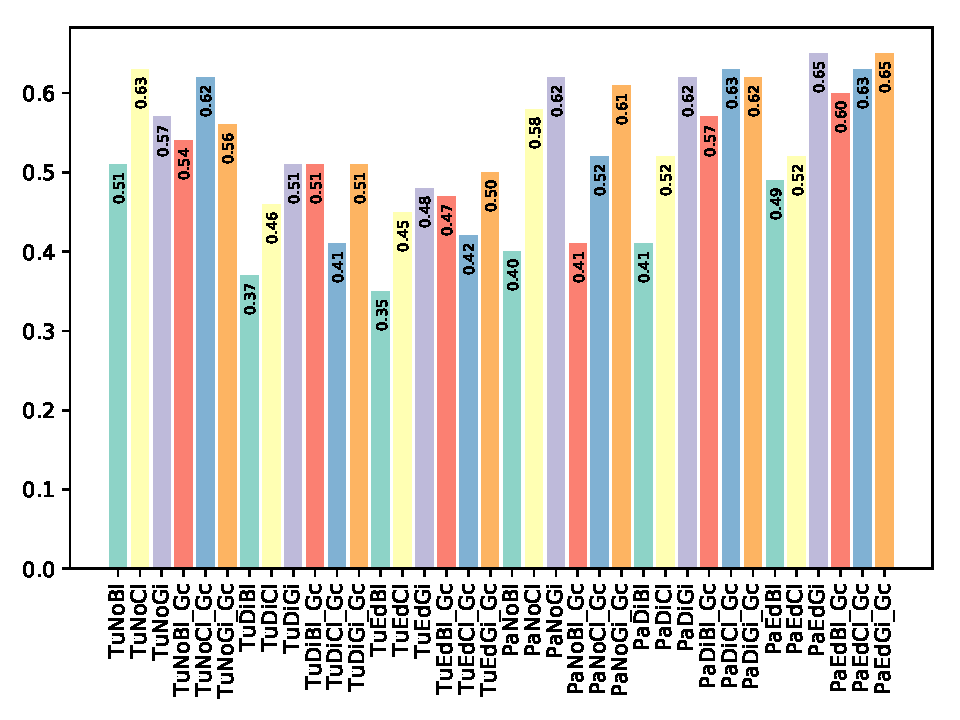
\includegraphics[page=1,scale=0.80]{img/Validation_generale_DEI.pdf}}
\captionof{figure}{Valori di V-measure delle partizioni generate}
\label{img:graficovmeasure}
\end{minipage}
}

% TODO da qualche parte 4 grafi, layout fisso colori variabili in base ai diversi modi di generare
% cluster. (volendo 24 grafi colorati a gruppi di 4)

% \clearpage

\subsection{Analisi}

\subsubsection{Confronto tra i metodi di estrazione}

I valori di \textit{V-measure}, aggregati per metodo di estrazione dei dati ed unione dei nodi, sono
riassunti in figura \ref{img:vmeasureestrazione}.

I grafi generati considerando solo i paper scritti da autori con almeno un affiliation padovana
hanno un valore medio di \textit{V-measure} di $0.56$, lievemente superiore al valore medio ottenuto
dai grafi generati considerando tutti i paper estratti, pari a $0.49$.

Il valore della \textit{V-measure} del grafo generato considerando tutti i paper estratti ed unendo
i nodi per nome è fra i più alti, ma ciò non corrisponde a un grafo ben rappresentativo della rete
di autori del DEI, per i motivi illustrati in \ref{ssc:padovani}.

% figura grafico v-measure aggregata per strada
\begin{figure}[H]
    \begin{minipage}[c]{0.60\textwidth}
    \setlength{\fboxrule}{0pt}	%barbatrucco per far sparire il bordo della box
    \fbox{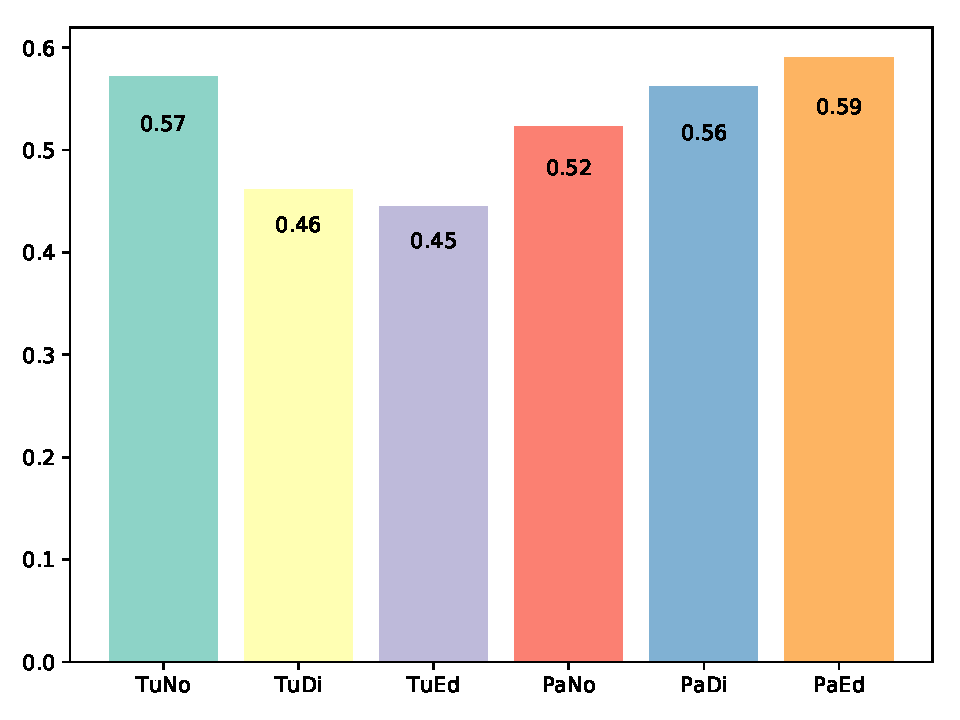
\includegraphics[page=1,scale=0.40]{img/Validation_Unione_DEI.pdf}}
    \end{minipage}
    % \hfill
    \begin{minipage}[c]{0.32\textwidth}
    \caption{Medie dei valori di \textit{V-measure} aggregate per metodo di estrazione degli autori
        e per metodo di unione dei nodi}
    \label{img:vmeasureestrazione}
    \end{minipage}
\end{figure}

% \centerline{
% \begin{minipage}{1.15\textwidth}
% \setlength{\fboxrule}{0pt}	%barbatrucco per far sparire il bordo della box
% \fbox{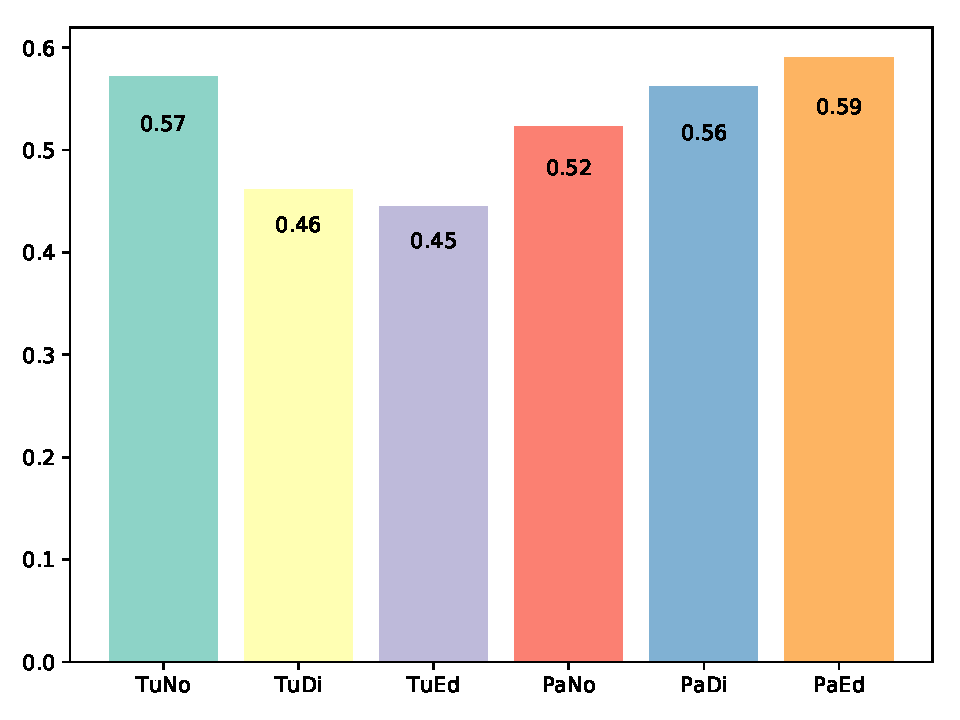
\includegraphics[page=1,scale=0.40]{img/Validation_Unione_DEI.pdf}}
% \captionof{figure}{Medie dei valori di \textit{V-measure} aggregate per metodo di estrazione}
% \label{img:vmeasureestrazione}
% \end{minipage}
% }

% \clearpage

\subsubsection{Confronto tra i metodi di community detection}

I valori di \textit{V-measure}, aggregati per algoritmo di generazione dei cluster, sono riassunti
in figura \ref{img:vmeasurecluster}.

Il metodo Girvan-Newman si è rivelato essere il migliore in termini di \textit{V-measure}, sia
quando applicato all'intero grafo, sia quando applicato solo alla componente centrale dello stesso.

Nel caso del metodo Blockmodel, si nota una differenza tra l'analisi dell'intero grafo e della sua
componente centrale, ed è stata rilevata una migliore efficacia del metodo nel secondo caso.

\begin{figure}[H]
    \begin{minipage}[c]{0.60\textwidth}
    \setlength{\fboxrule}{0pt}	%barbatrucco per far sparire il bordo della box
    \fbox{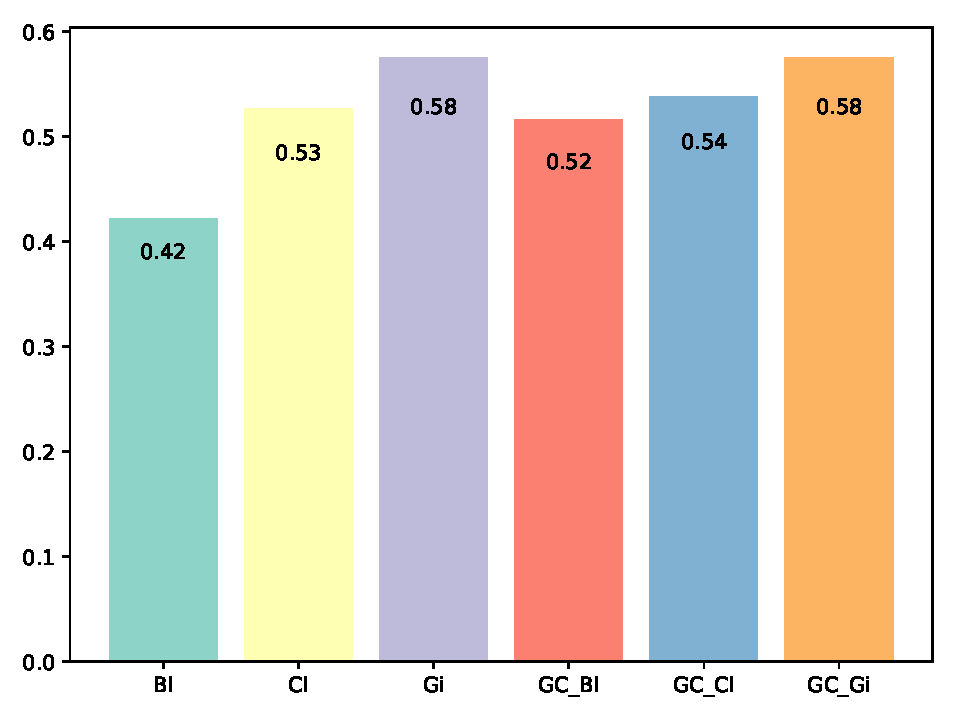
\includegraphics[page=1,scale=0.40]{img/Validation_Comunita_DEI.pdf}}
    \end{minipage}
    % \hfill
    \begin{minipage}[c]{0.32\textwidth}
    \caption{Medie dei valori di V-measure aggregate per algoritmo di generazione cluster }
    \label{img:vmeasurecluster}
    \end{minipage}
\end{figure}

% \centerline{
% \begin{minipage}{1.15\textwidth}
% \setlength{\fboxrule}{0pt}	%barbatrucco per far sparire il bordo della box
% \fbox{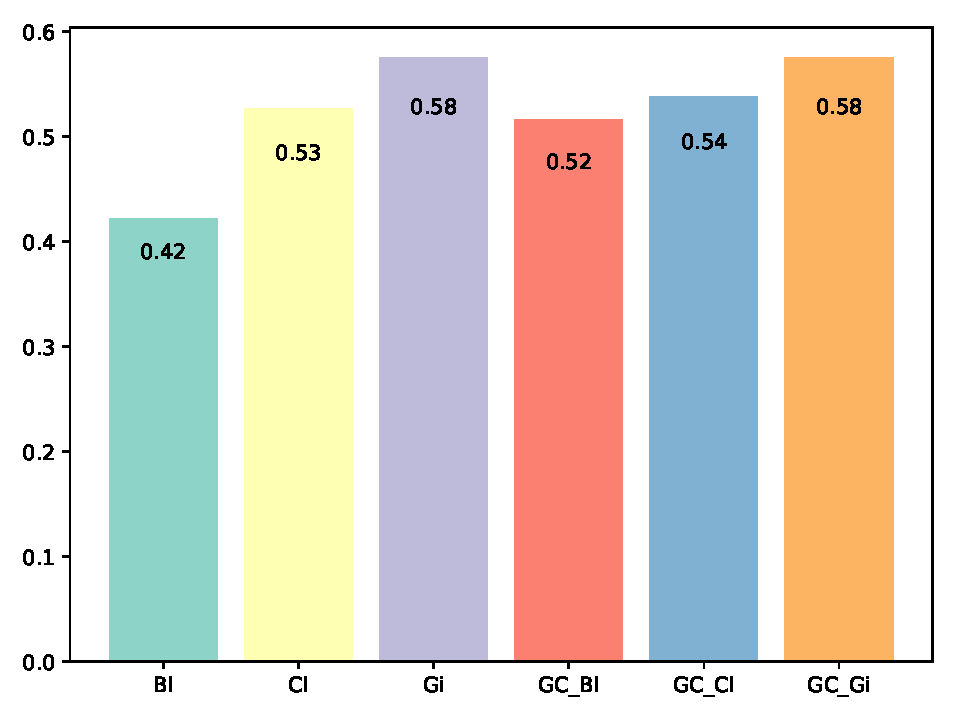
\includegraphics[page=1,scale=0.40]{img/Validation_Comunita_DEI.pdf}}
% \captionof{figure}{Medie dei valori di V-measure aggregate per algoritmo di generazione cluster}
% \label{img:vmeasurecluster}
% \end{minipage}
% }

Nelle pagine successive sono riportati i grafi che hanno ottenuto i valori migliori di
\textit{V-measure}

In figura \ref{fig:grafipadovaniedge} sono presenti i grafi relativi ai grafi generati considerando
solo gli autori con almeno un'affiliation padovana, unendo i nodi seguendo la strategia dei nodi
adiacenti. In figura \ref{fig:grafipadovaniedgeaggregati} i cluster degli stessi grafi sono stati
aggregati per evidenziare le relazioni tra le comunità del grafo.

In figura \ref{fig:grafigirvanaggregati} sono riportati i cluster ottenuti applicando l'algoritmo di
Girvan e Newman alle componenti centrali dei grafi generati in tutti i possibili modi.

\clearpage
\begin{figure}[ht]
    \centering
        \begin{subfigure}[b]{0.5\textwidth}
            \centering
            \setlength{\fboxrule}{0pt} % barbatrucco per far sparire il bordo della box
            % \fbox{\includegraphics[page=1,scale=0.30]{img/Aggregati/GrafoAggregato_padovani_edge_girvan_DEI.pdf}}
            \fbox{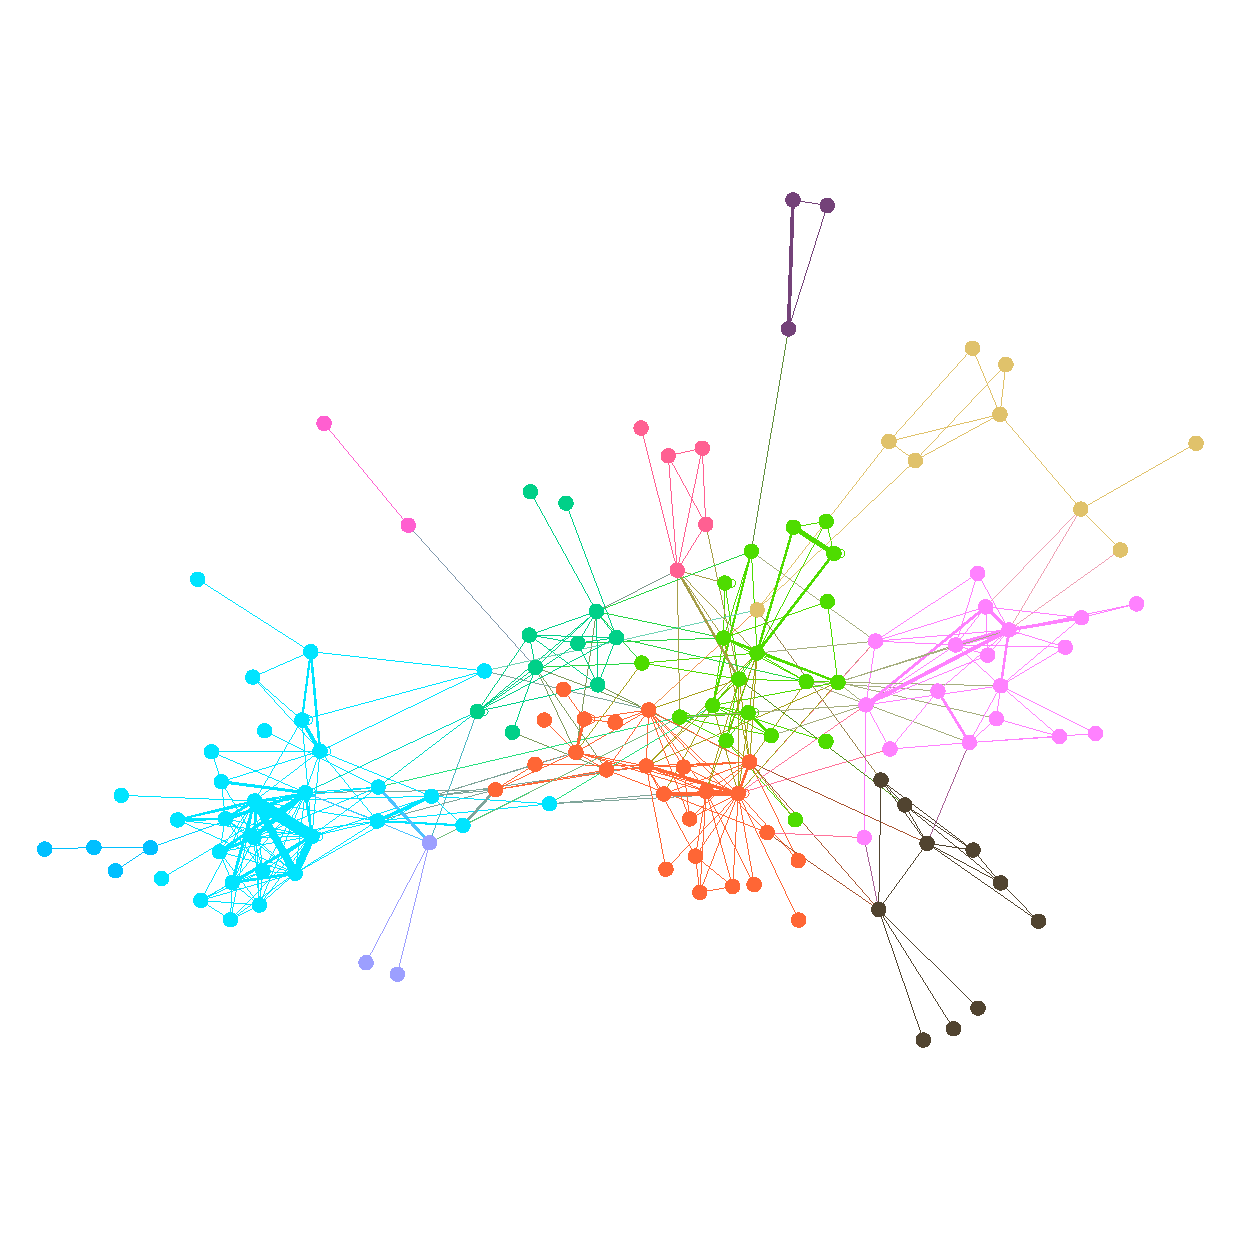
\includegraphics[page=1,scale=0.30]{img/Aggregati/GrafoPadovaniEdgeGirvan.pdf}}
            \caption{Girvan Newmann}
        \end{subfigure}%
        ~
        \begin{subfigure}[b]{0.5\textwidth}
            \centering
            \setlength{\fboxrule}{0pt} % barbatrucco per far sparire il bordo della box
            \fbox{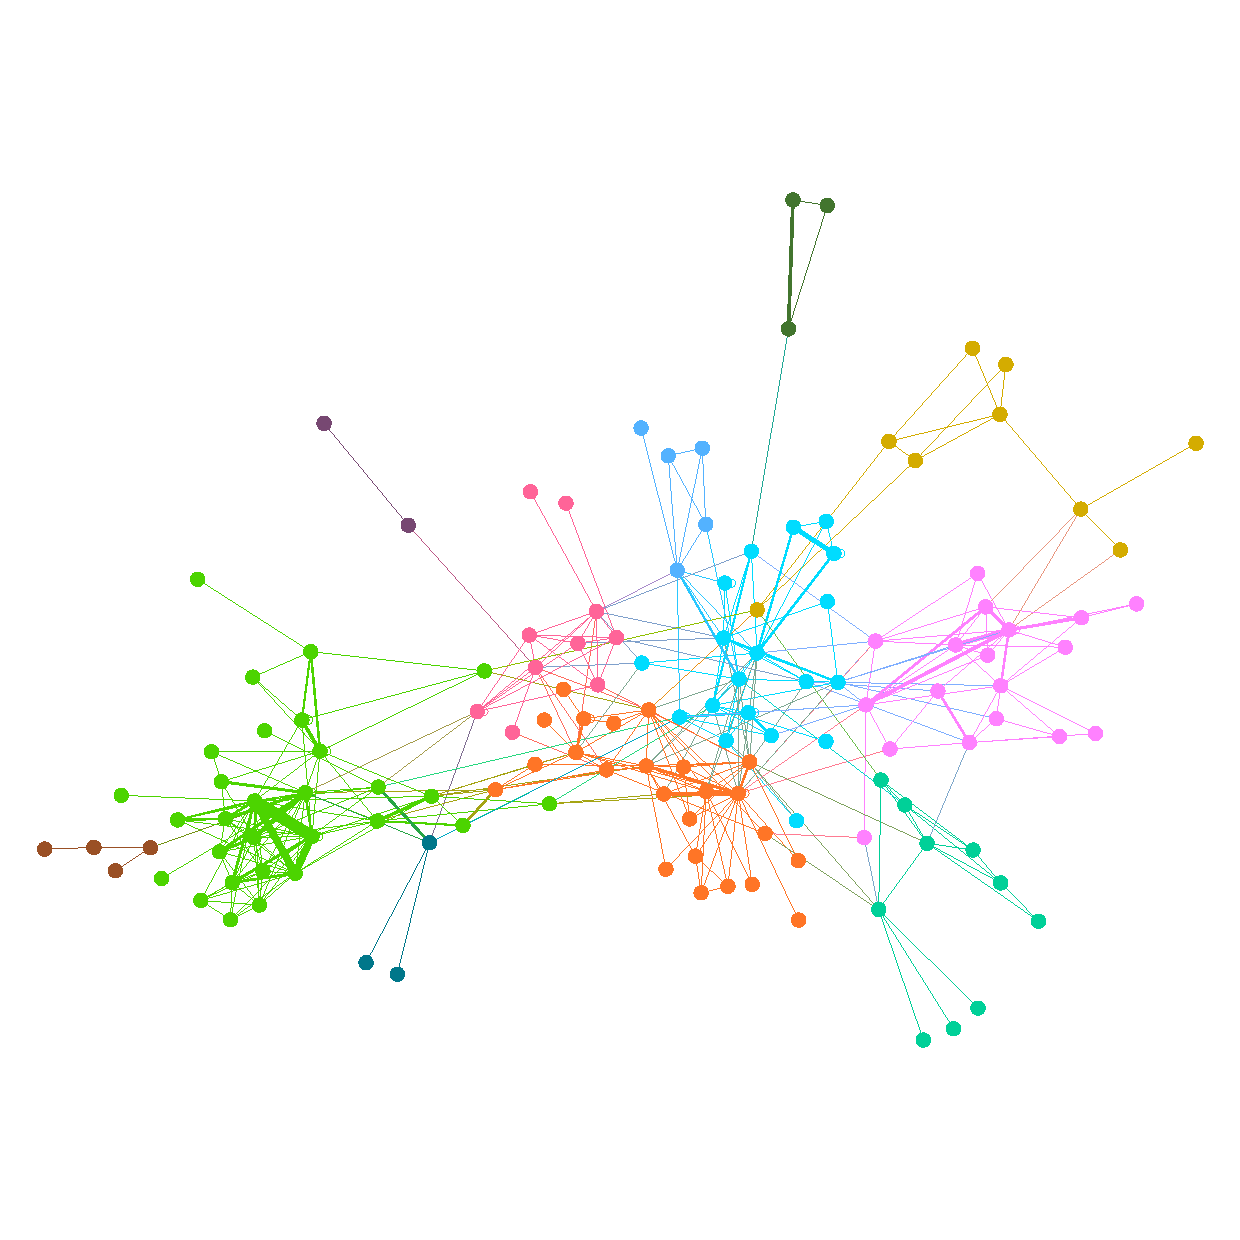
\includegraphics[page=1,scale=0.30]{img/Aggregati/GrafoPadovaniEdgeGirvanGiant.pdf}}
            \caption{GN - Componente centrale}
        \end{subfigure}
        \\
        \begin{subfigure}[b]{0.5\textwidth}
            \centering
            \setlength{\fboxrule}{0pt} % barbatrucco per far sparire il bordo della box
            \fbox{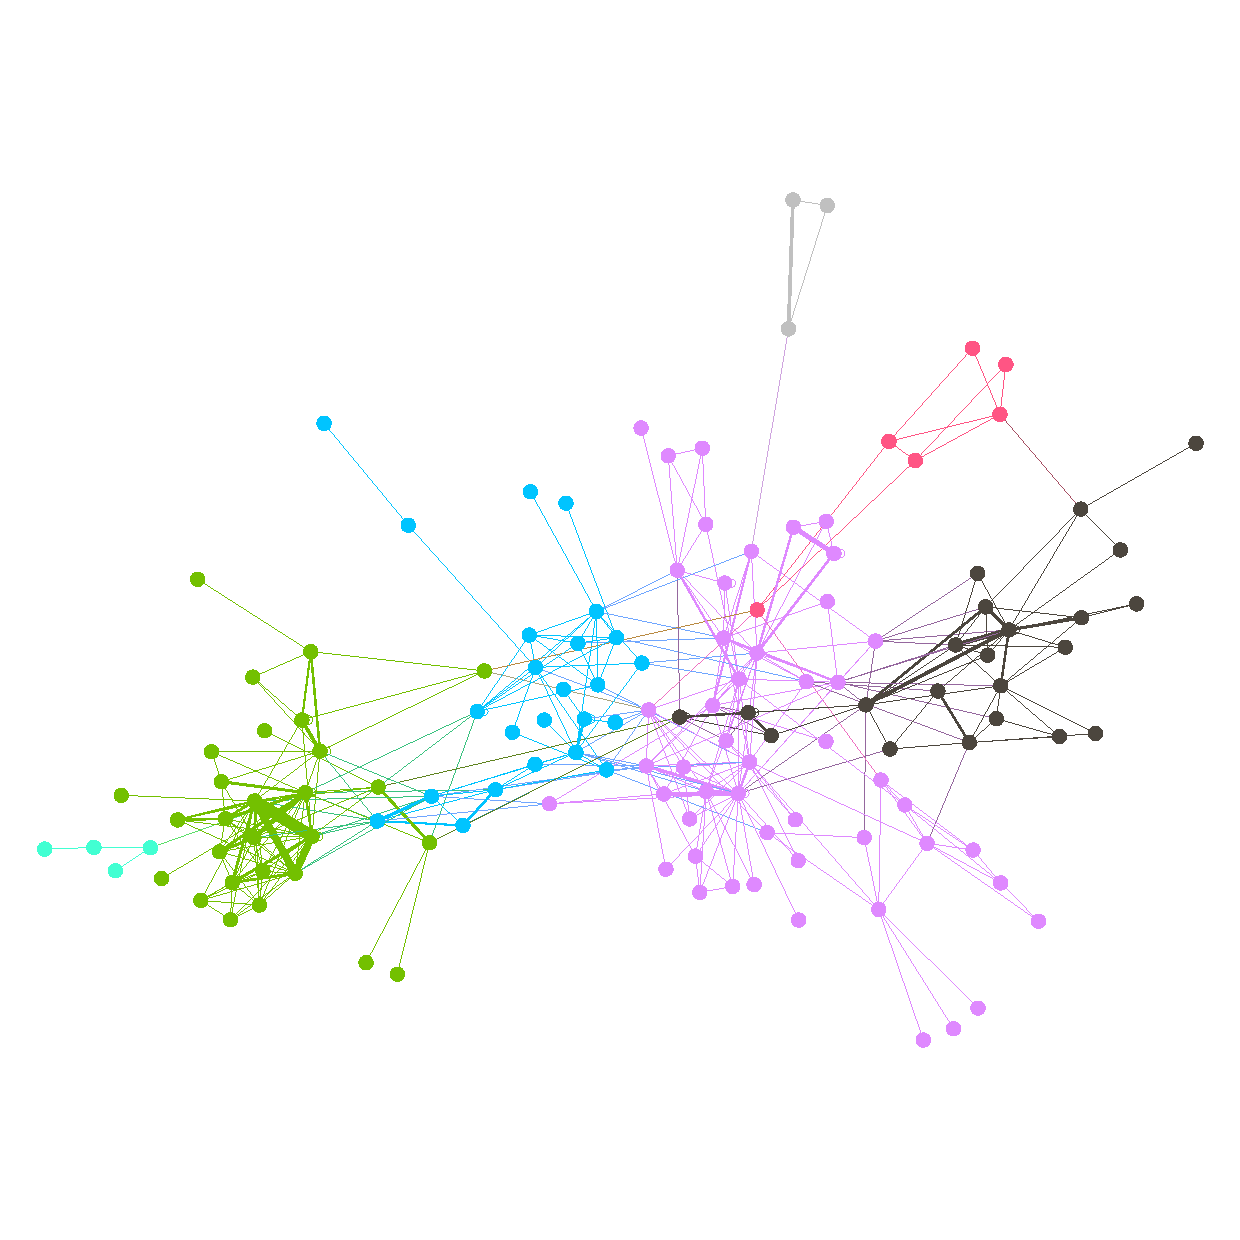
\includegraphics[page=1,scale=0.30]{img/Aggregati/GrafoPadovaniEdgeClanemo.pdf}}
            \caption{Clauset Newman Moore}
        \end{subfigure}%
        ~
        \begin{subfigure}[b]{0.5\textwidth}
            \centering
            \setlength{\fboxrule}{0pt} % barbatrucco per far sparire il bordo della box
            % \fbox{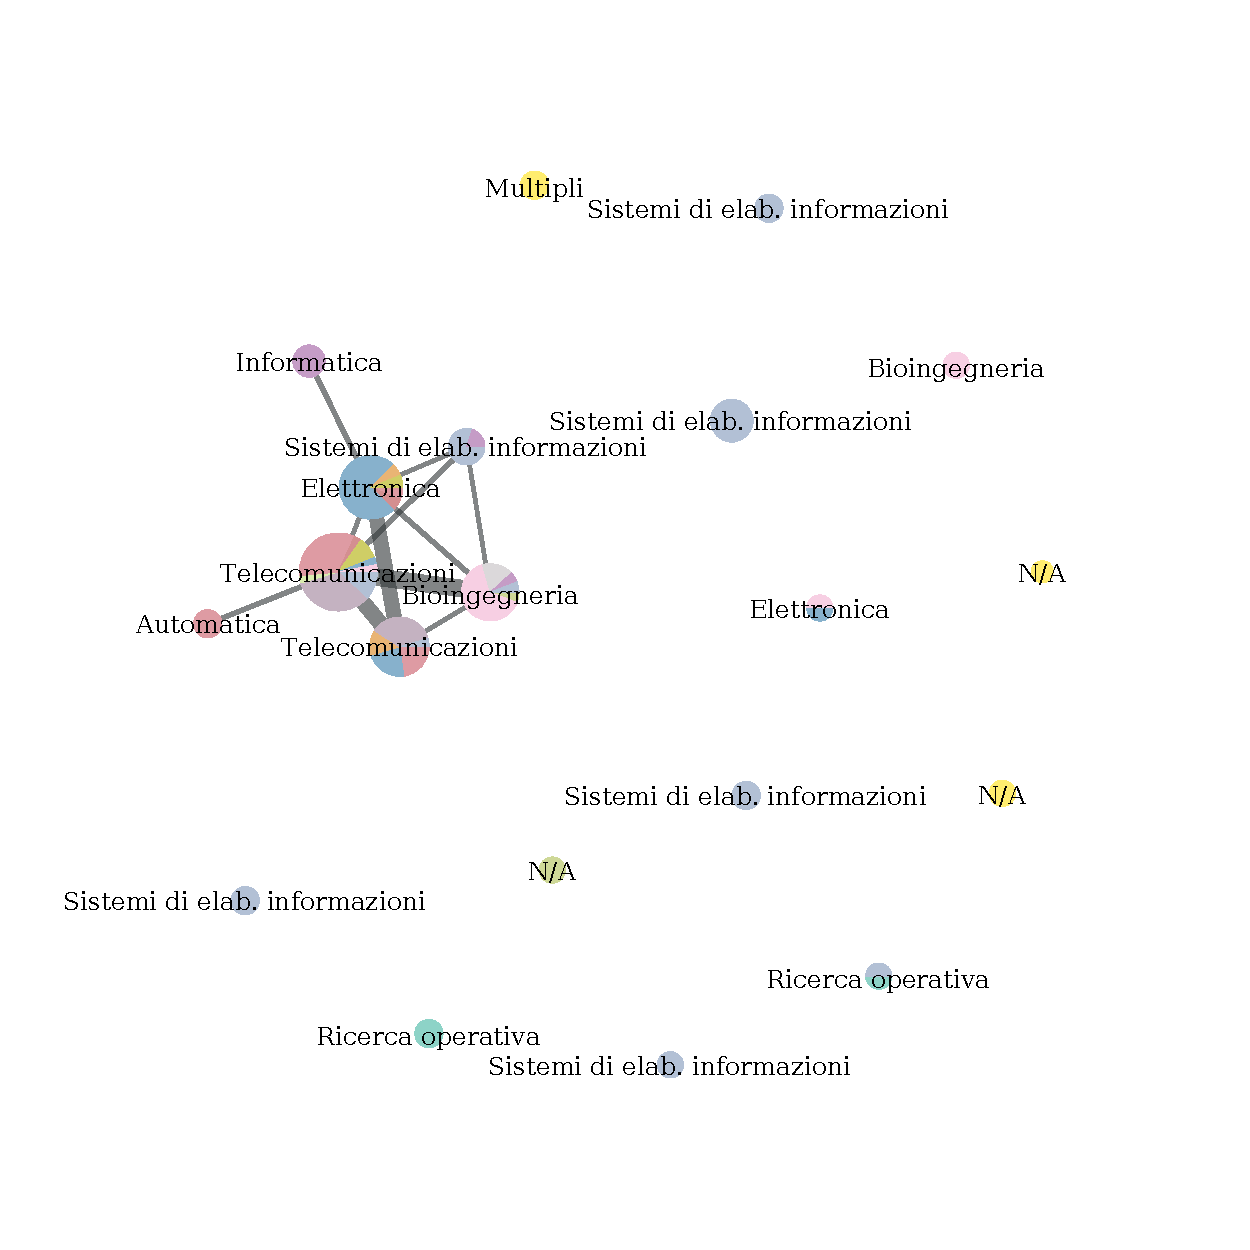
\includegraphics[page=1,scale=0.30]{img/Aggregati/GrafoAggregato_padovani_edge_clanemo_DEI.pdf}}
            \fbox{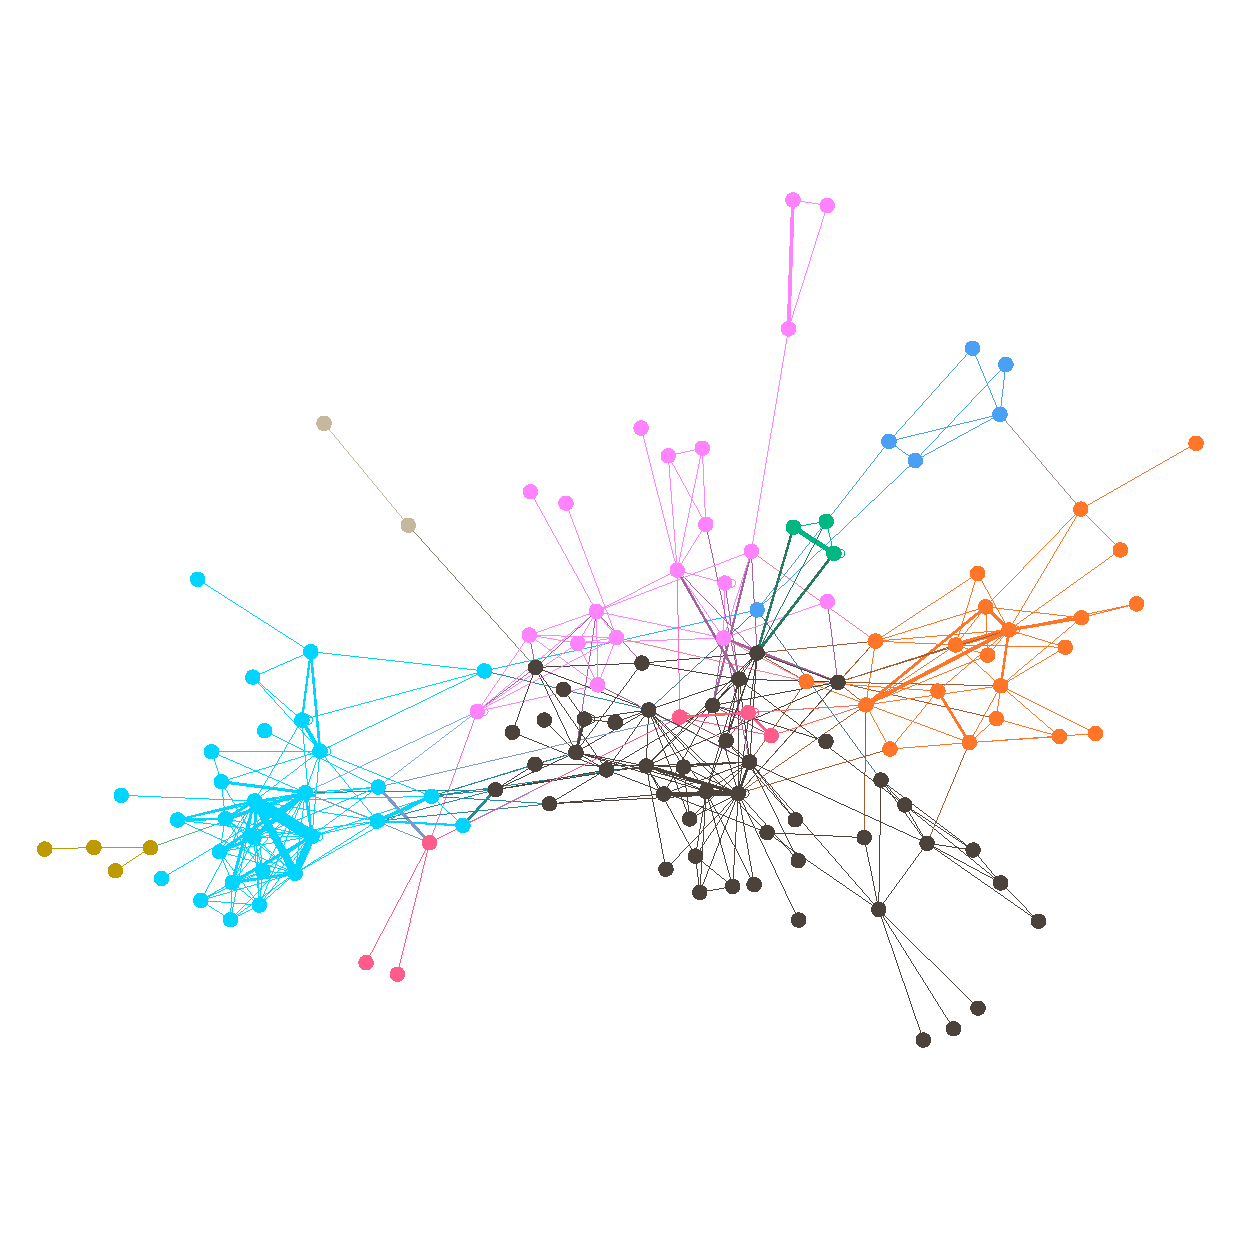
\includegraphics[page=1,scale=0.30]{img/Aggregati/GrafoPadovaniEdgeClanemoGiant.pdf}}
            \caption{CNM - componente centrale}
        \end{subfigure}%
        \\
        \begin{subfigure}[b]{0.5\textwidth}
            \centering
            \setlength{\fboxrule}{0pt} % barbatrucco per far sparire il bordo della box
            \fbox{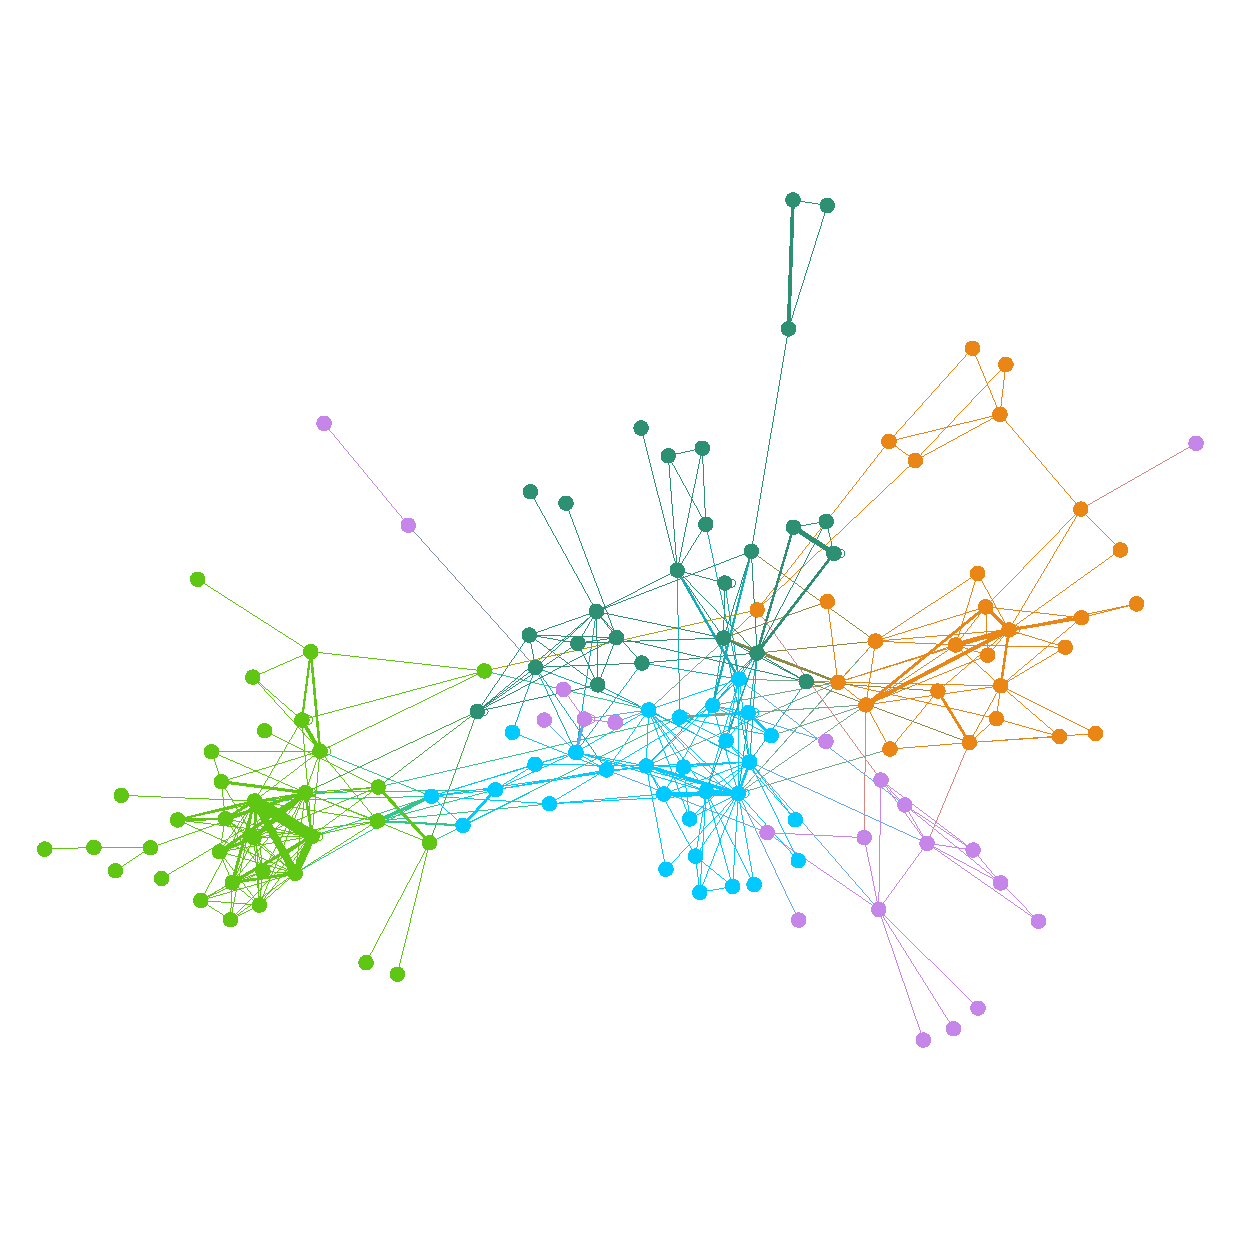
\includegraphics[page=1,scale=0.30]{img/Aggregati/GrafoPadovaniEdgeBlockmodel.pdf}}
            \caption{Block Model}
        \end{subfigure}%
        ~
        \begin{subfigure}[b]{0.5\textwidth}
            \centering
            \setlength{\fboxrule}{0pt} % barbatrucco per far sparire il bordo della box
            \fbox{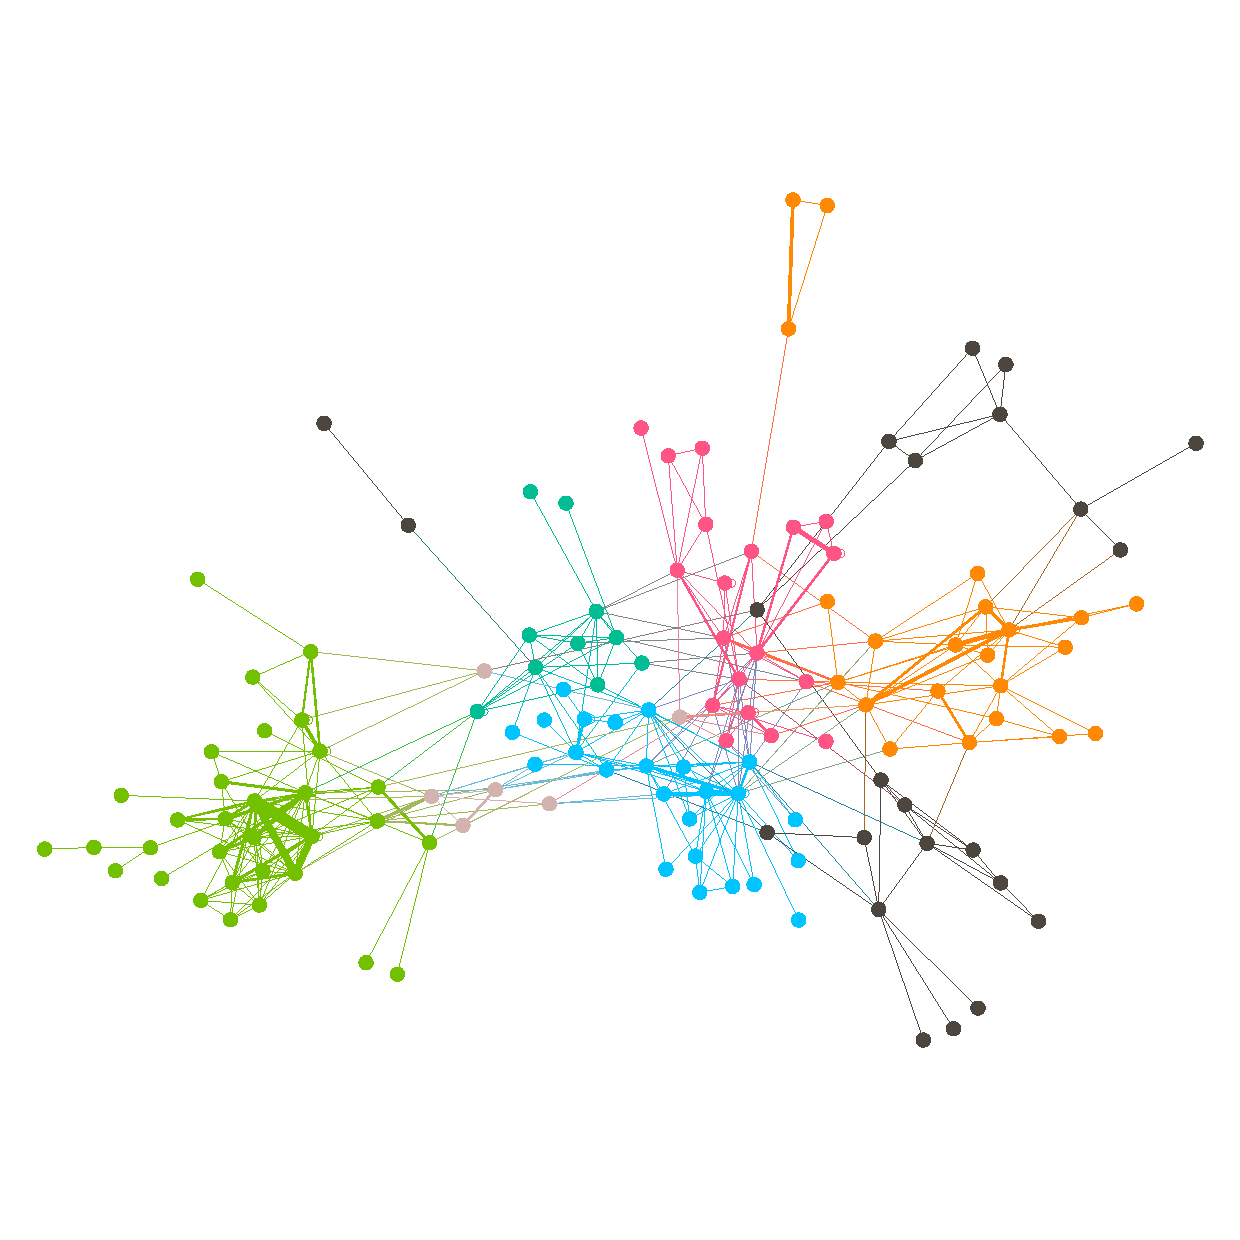
\includegraphics[page=1,scale=0.30]{img/Aggregati/GrafoPadovaniEdgeBlockmodelGiant.pdf}}
            \caption{BM - componente centrale}
        \end{subfigure}%
    \caption{Confronto delle suddivisioni in cluster del grafo degli autori con almeno un'affiliation
    padovana, dove i nodi sono stati uniti utilizzando la strategia per nodi adiacenti}
    \label{fig:grafipadovaniedge}
\end{figure}

\clearpage
\begin{figure}[ht]
    \centering
        \begin{subfigure}[b]{0.5\textwidth}
            \centering
            \setlength{\fboxrule}{0pt} % barbatrucco per far sparire il bordo della box
            % \fbox{\includegraphics[page=1,scale=0.30]{img/Aggregati/GrafoAggregato_padovani_edge_girvan_DEI.pdf}}
                \fbox{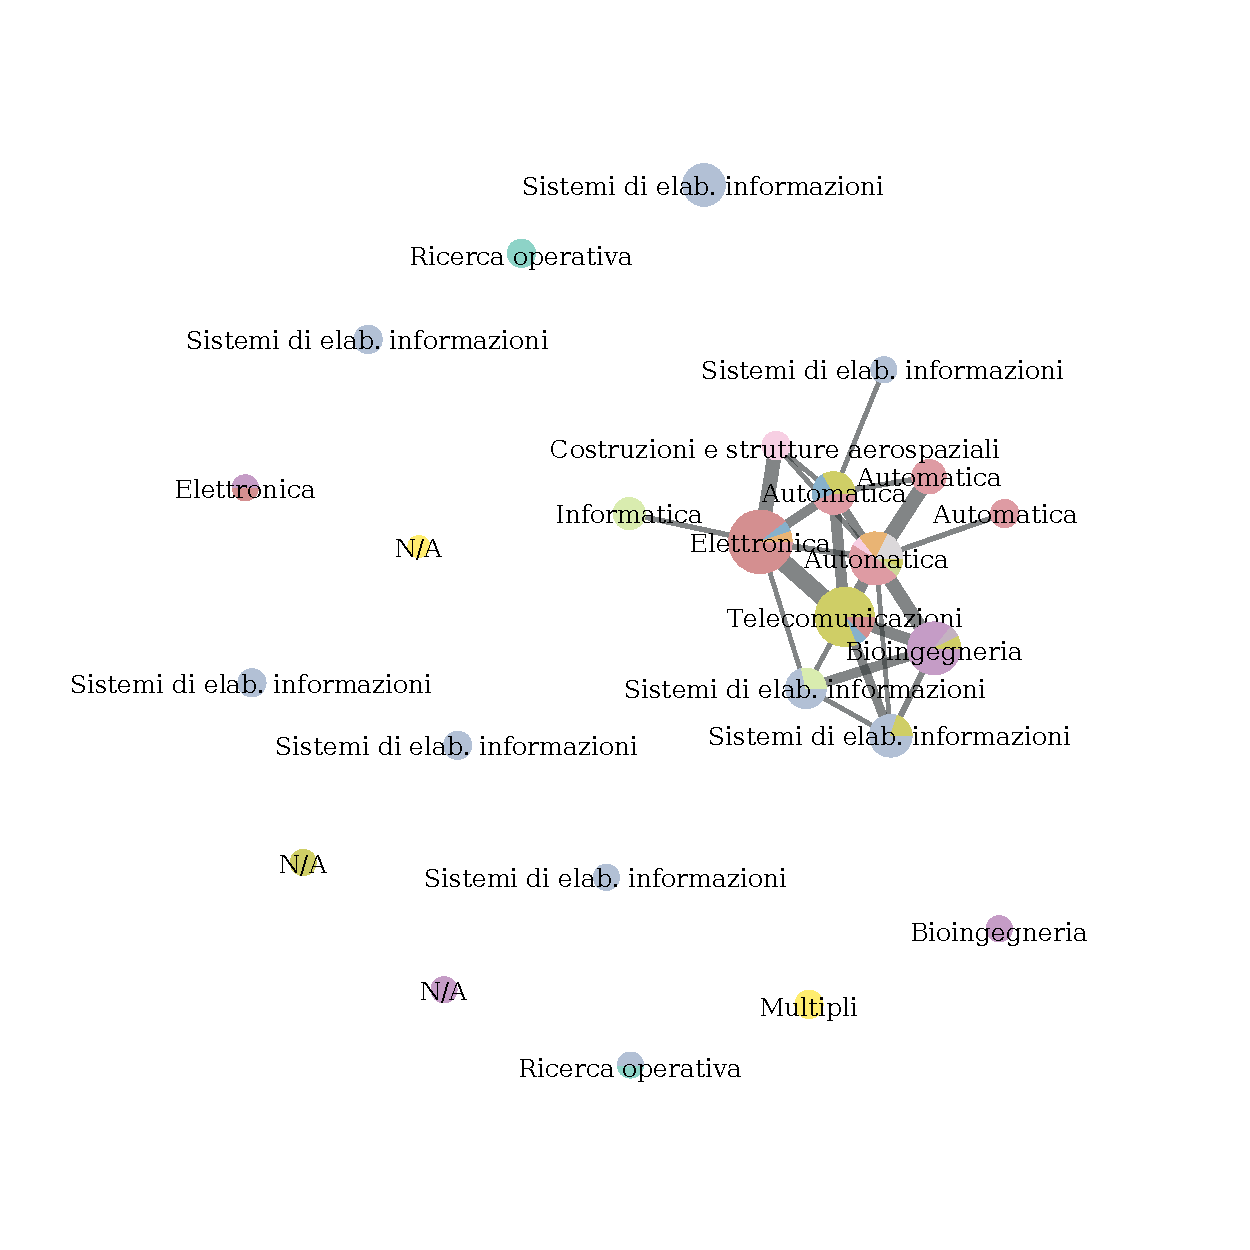
\includegraphics[page=1,scale=0.30]{img/Aggregati/GrafoAggregato_padovani_edge_girvnew_DEI.pdf}}
                \caption{Girvan Newmann}
            \end{subfigure}%
            ~
            \begin{subfigure}[b]{0.5\textwidth}
                \centering
                \setlength{\fboxrule}{0pt} % barbatrucco per far sparire il bordo della box
                \fbox{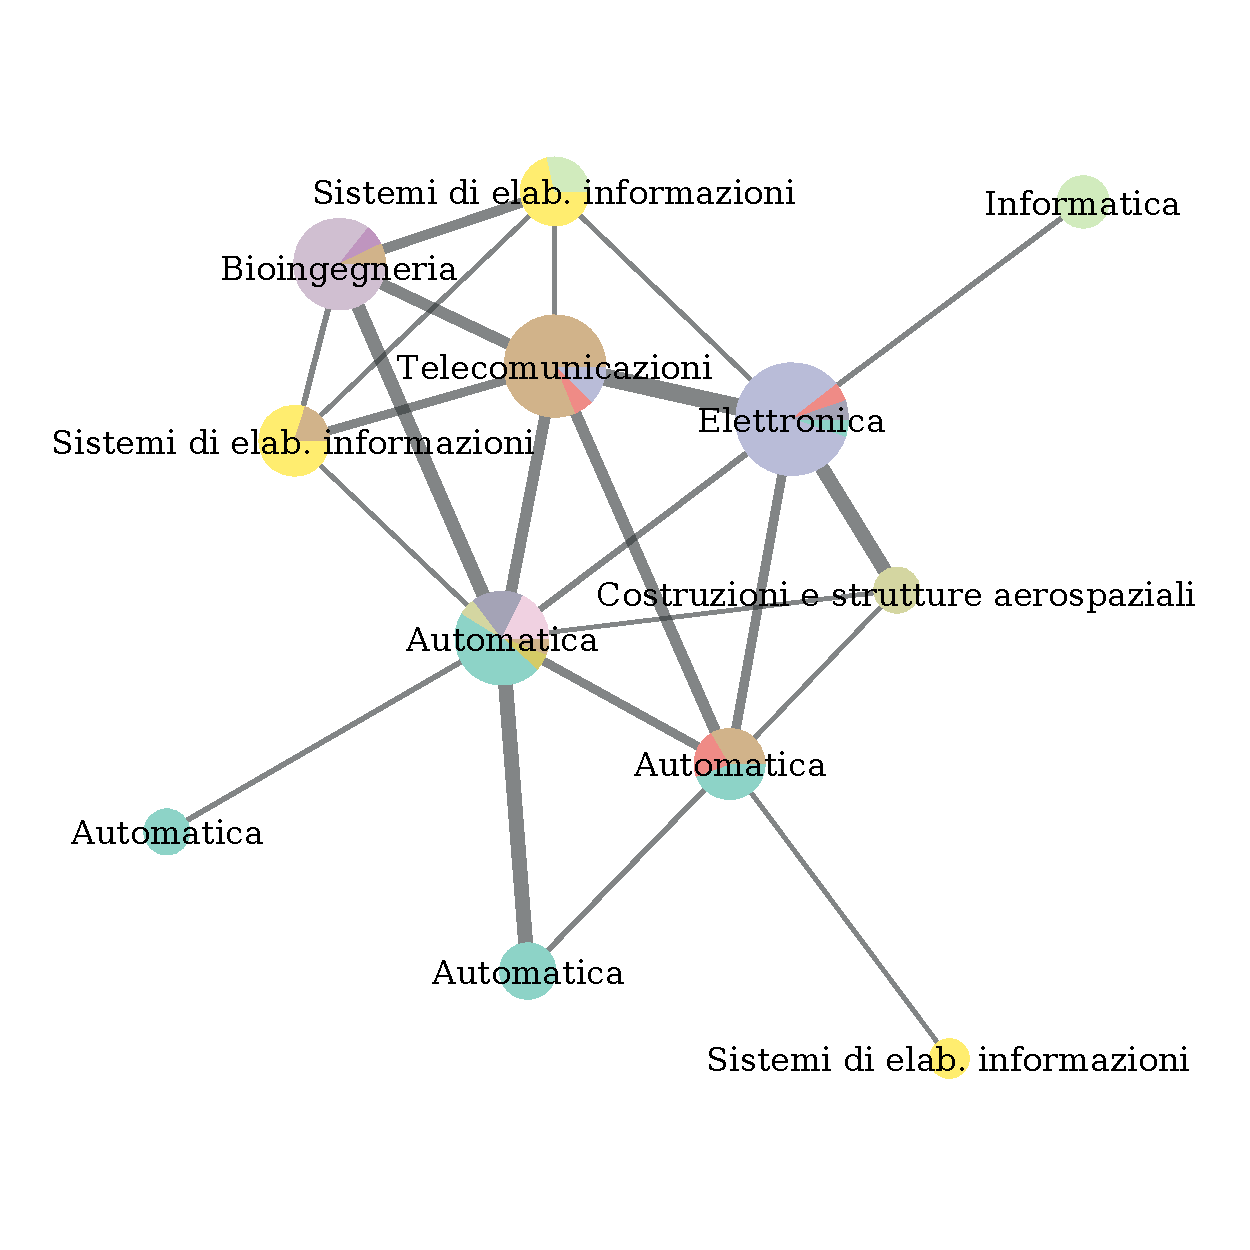
\includegraphics[page=1,scale=0.30]{img/Aggregati/GrafoAggregato_padovani_edge_Zgirvnew_DEI.pdf}}
                \caption{GN - Componente centrale}
            \end{subfigure}
            \\
            \begin{subfigure}[b]{0.5\textwidth}
                \centering
                \setlength{\fboxrule}{0pt} % barbatrucco per far sparire il bordo della box
                \fbox{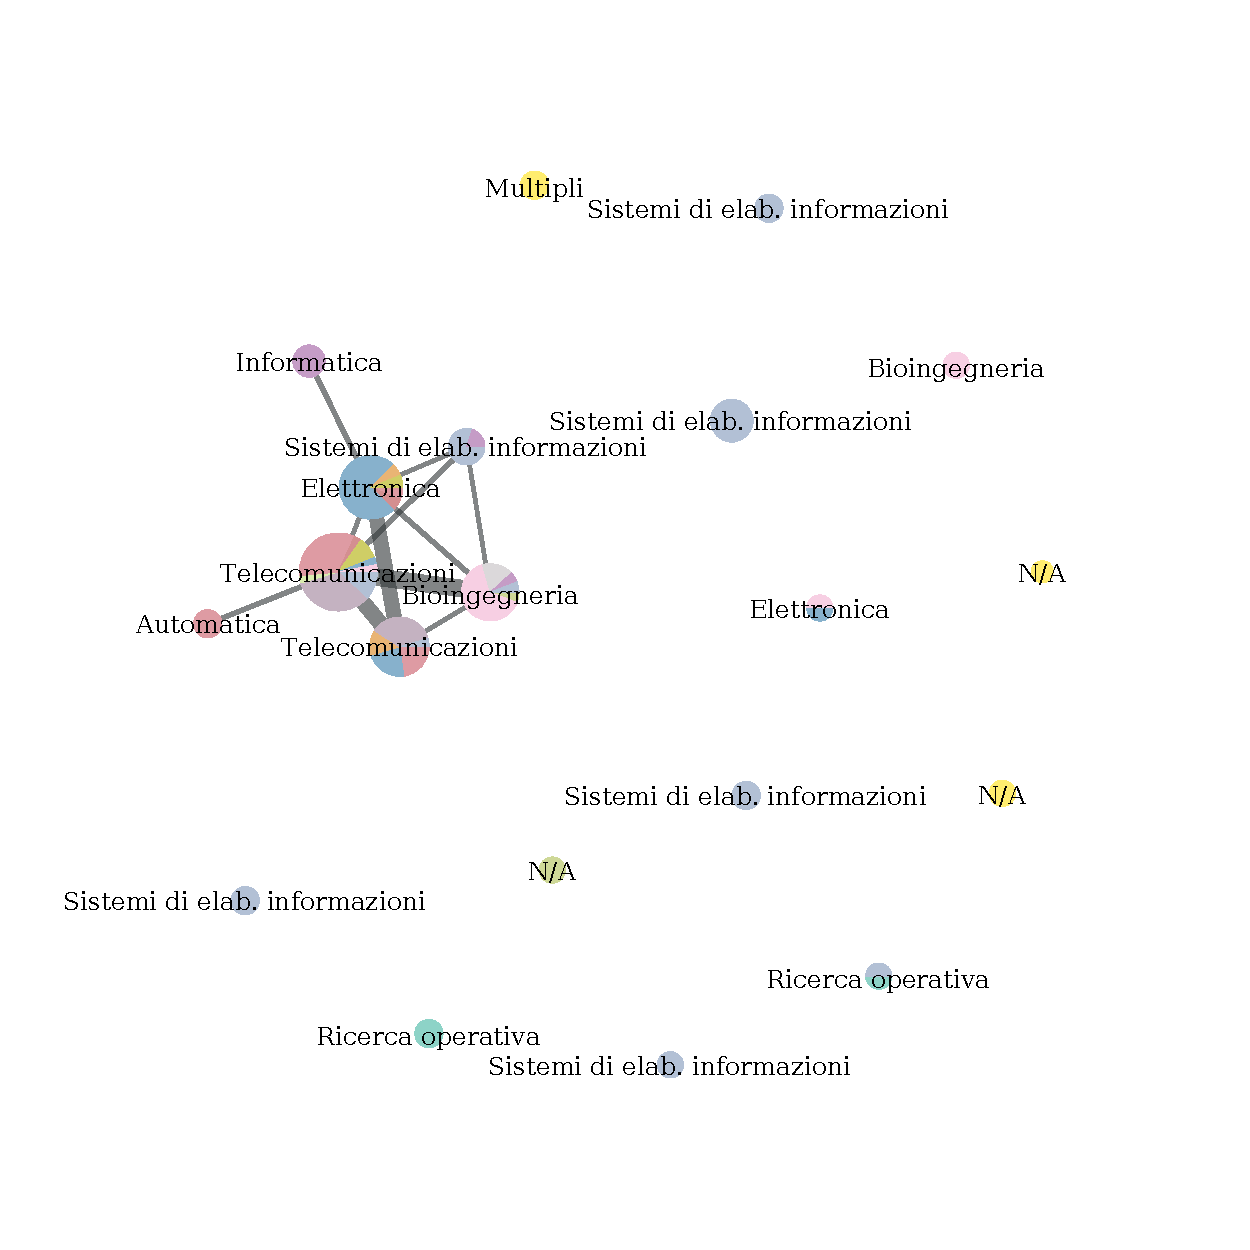
\includegraphics[page=1,scale=0.30]{img/Aggregati/GrafoAggregato_padovani_edge_clanemo_DEI.pdf}}
                \caption{Clauset Newman Moore}
            \end{subfigure}%
            ~
            \begin{subfigure}[b]{0.5\textwidth}
                \centering
                \setlength{\fboxrule}{0pt} % barbatrucco per far sparire il bordo della box
                % \fbox{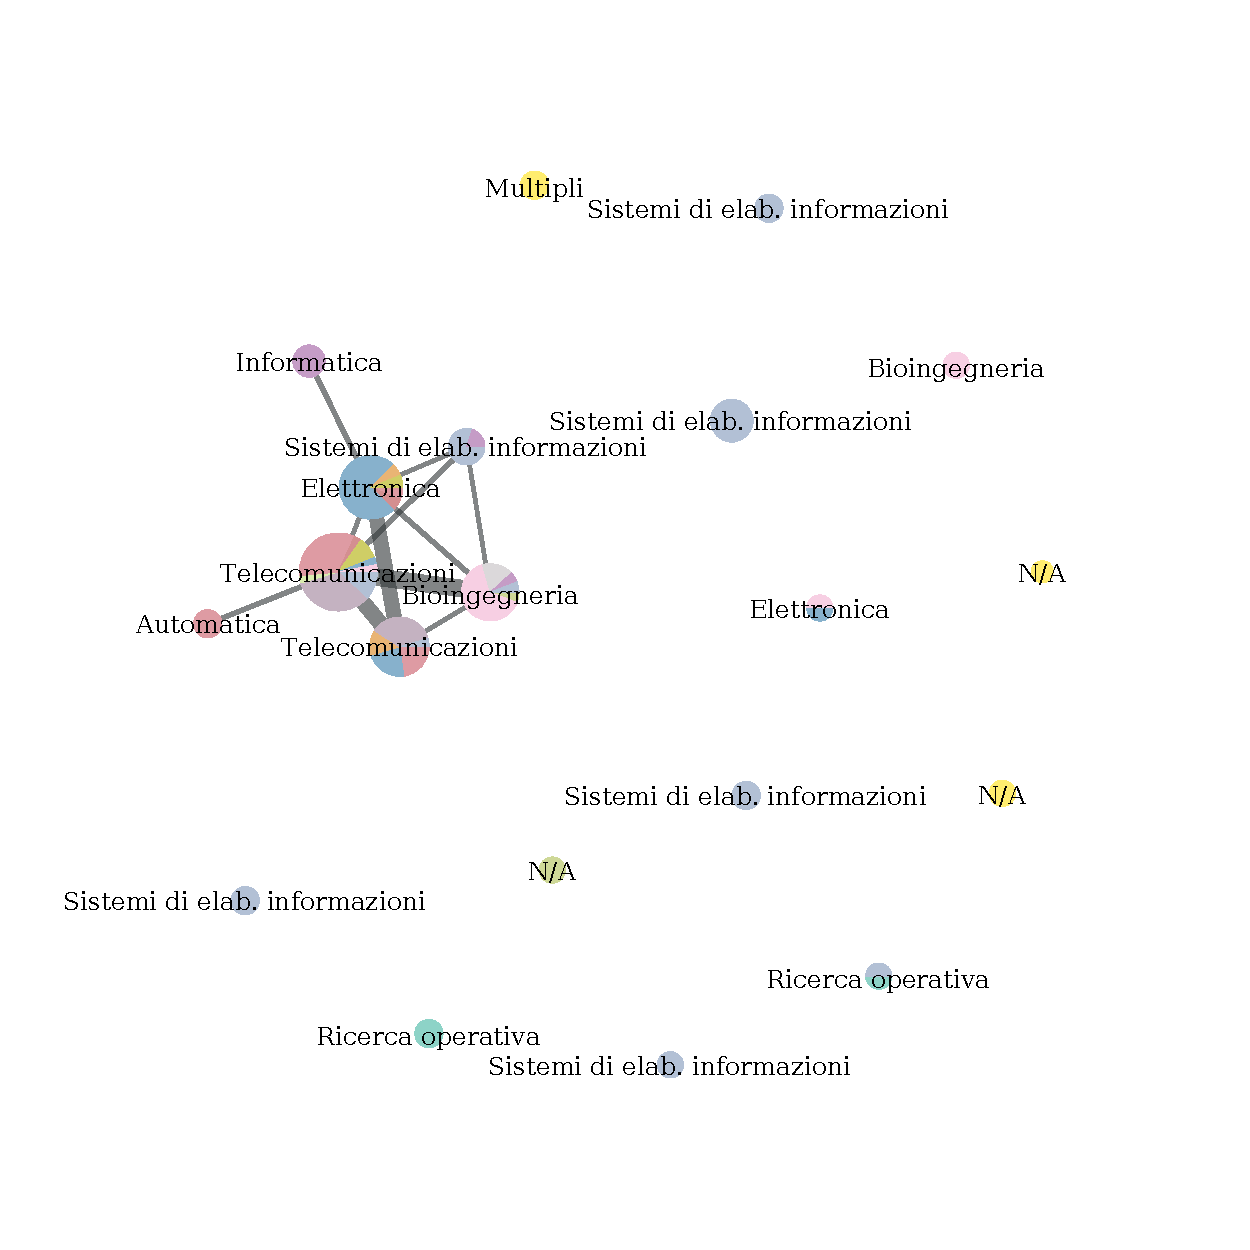
\includegraphics[page=1,scale=0.30]{img/Aggregati/GrafoAggregato_padovani_edge_clanemo_DEI.pdf}}
                \fbox{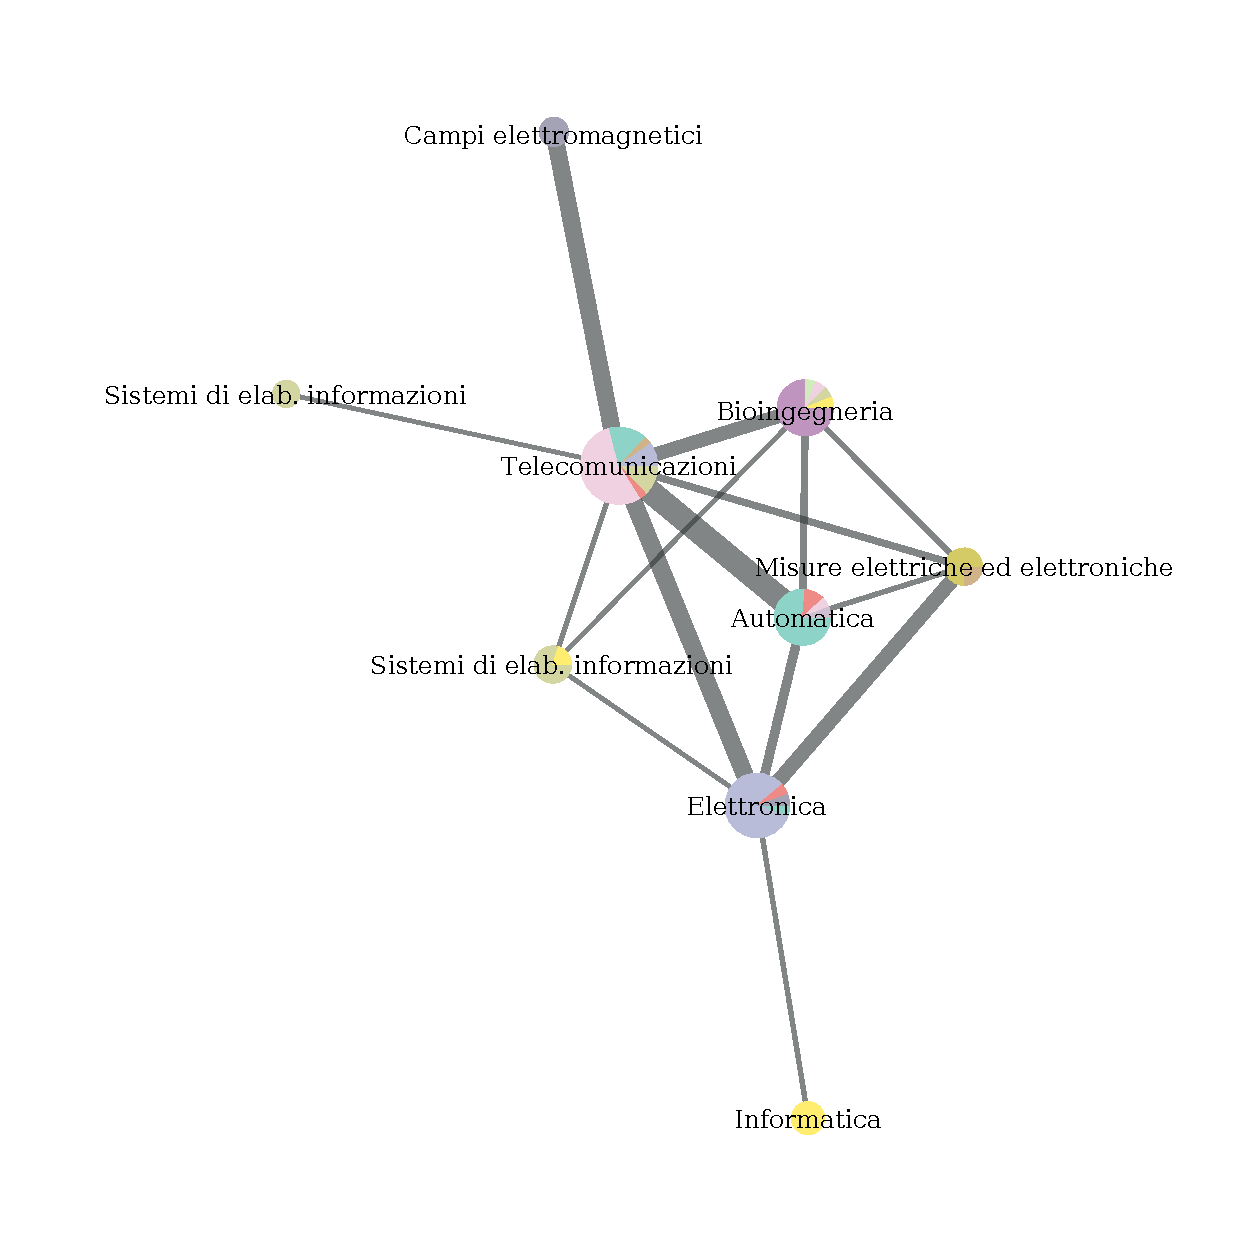
\includegraphics[page=1,scale=0.30]{img/Aggregati/GrafoAggregato_padovani_edge_Zclanemo_DEI.pdf}}
                \caption{CNM - componente centrale}
            \end{subfigure}%
            \\
            \begin{subfigure}[b]{0.5\textwidth}
                \centering
                \setlength{\fboxrule}{0pt} % barbatrucco per far sparire il bordo della box
                \fbox{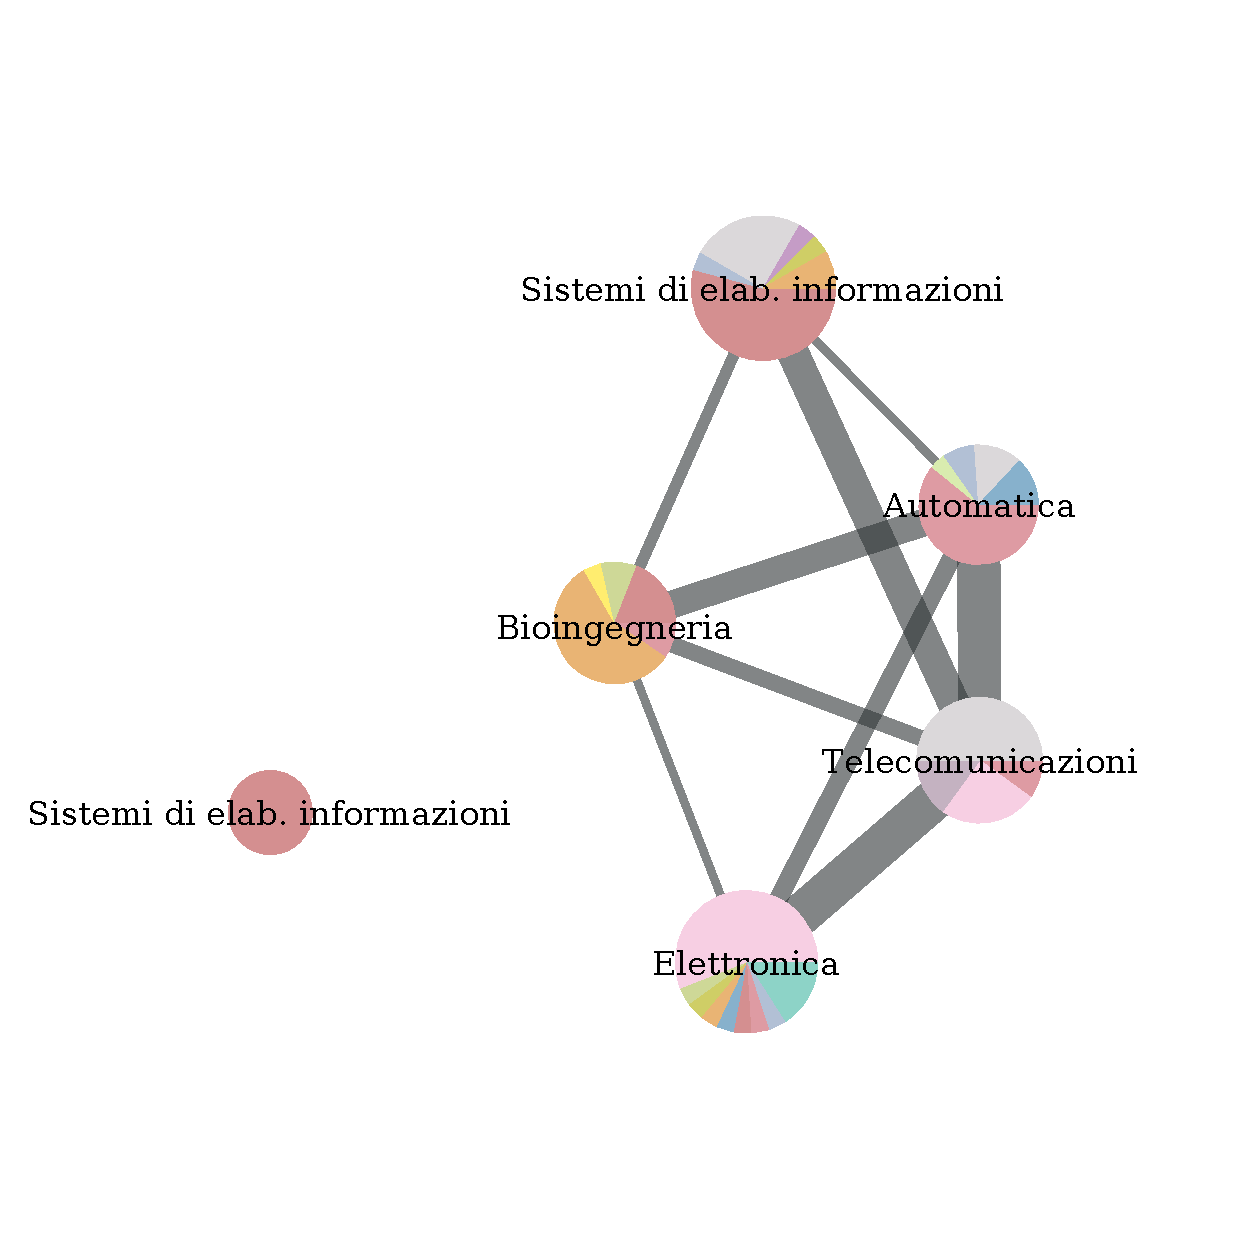
\includegraphics[page=1,scale=0.30]{img/Aggregati/GrafoAggregato_padovani_edge_blockmodel_DEI.pdf}}
                \caption{Block Model}
            \end{subfigure}%
            ~
            \begin{subfigure}[b]{0.5\textwidth}
                \centering
                \setlength{\fboxrule}{0pt} % barbatrucco per far sparire il bordo della box
                \fbox{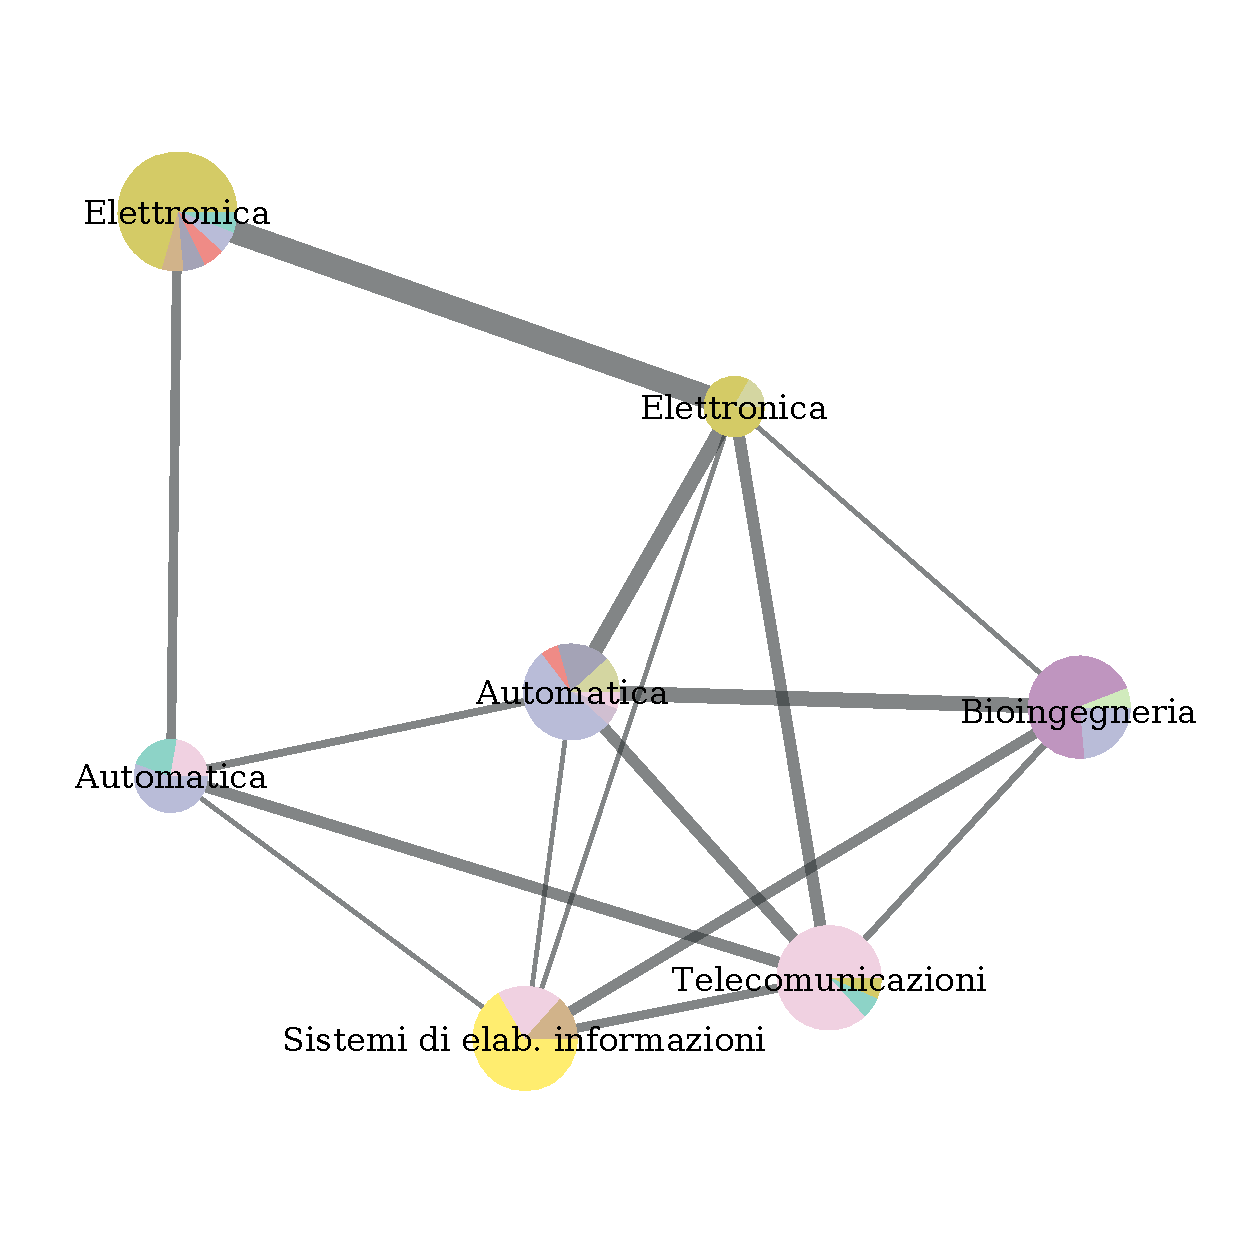
\includegraphics[page=1,scale=0.30]{img/Aggregati/GrafoAggregato_padovani_edge_Zblockmodel_DEI.pdf}}
                \caption{BM - componente centrale}
        \end{subfigure}%
    \caption{Confronto delle suddivisioni in cluster del grafo degli autori con almeno un'affiliation
    padovana, dove i nodi sono stati uniti utilizzando la strategia per nodi adiacenti; i cluster sono
    stati aggregati in nodi, i colori dei nodi indicano la suddivisione in classi dei cluster;
    l'etichetta corrisponde alla classe predominante nel cluster}
    \label{fig:grafipadovaniedgeaggregati}
\end{figure}

\clearpage
\begin{figure}[ht]
    \centering
        \begin{subfigure}[b]{0.5\textwidth}
                \centering
                \setlength{\fboxrule}{0pt} % barbatrucco per far sparire il bordo della box
                \fbox{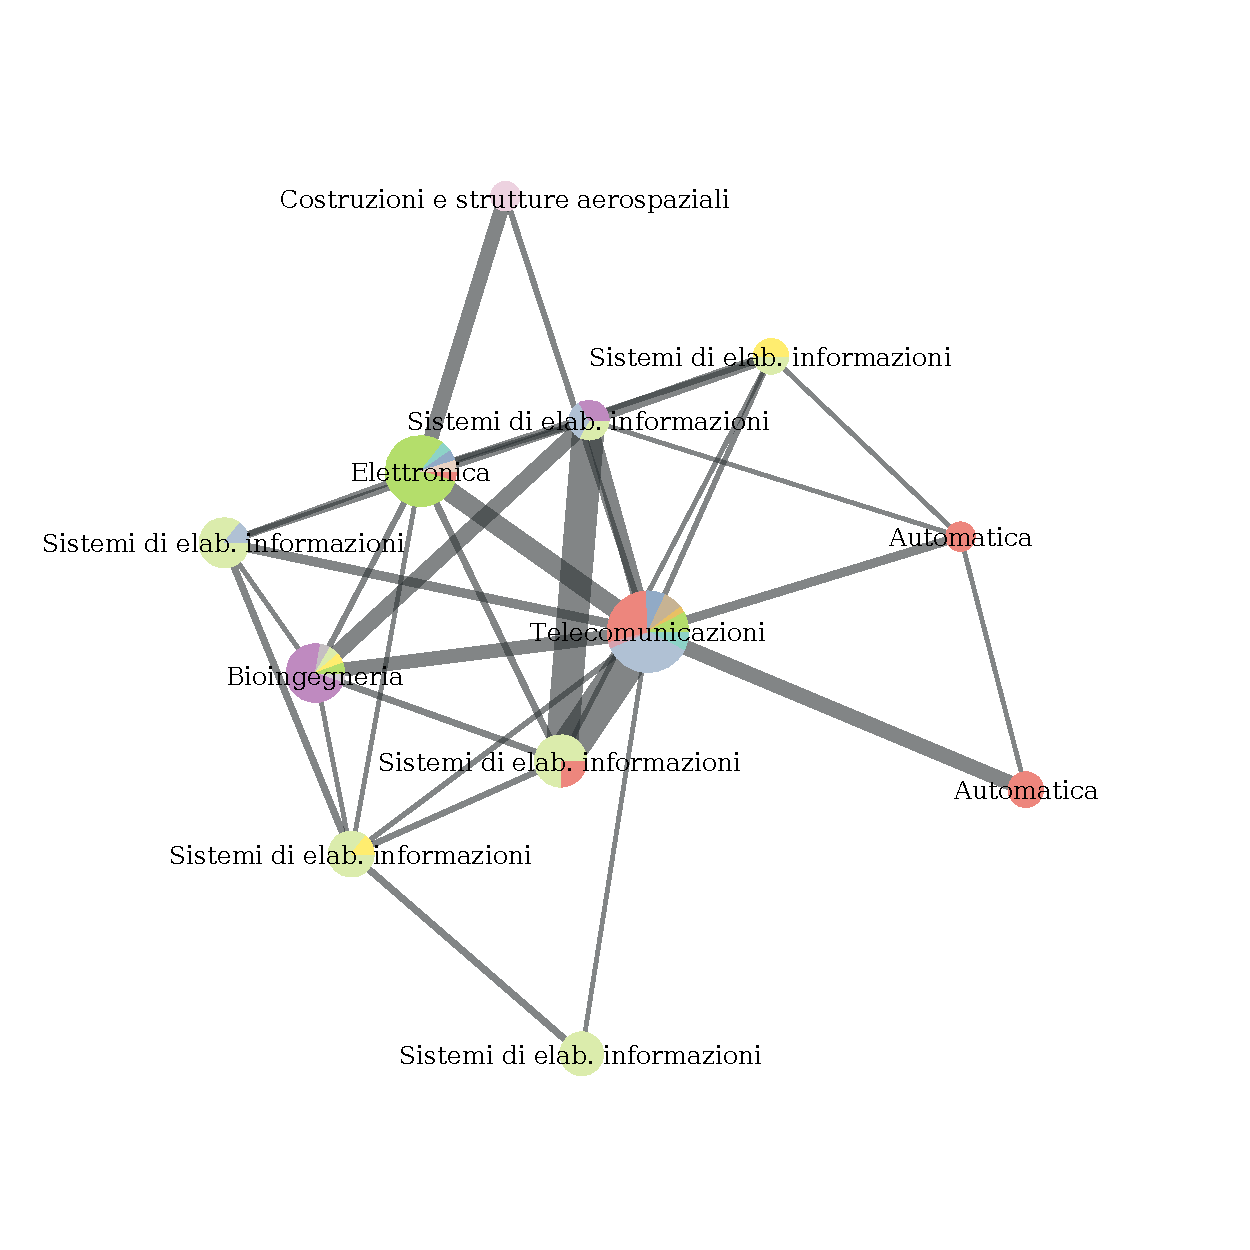
\includegraphics[page=1,scale=0.30]{img/Aggregati/GrafoAggregato_tutti_nomi_Zgirvnew_DEI.pdf}}
                \caption{Tutti - uniti per nome}
            \end{subfigure}%
            ~
            \begin{subfigure}[b]{0.5\textwidth}
                \centering
                \setlength{\fboxrule}{0pt} % barbatrucco per far sparire il bordo della box
                \fbox{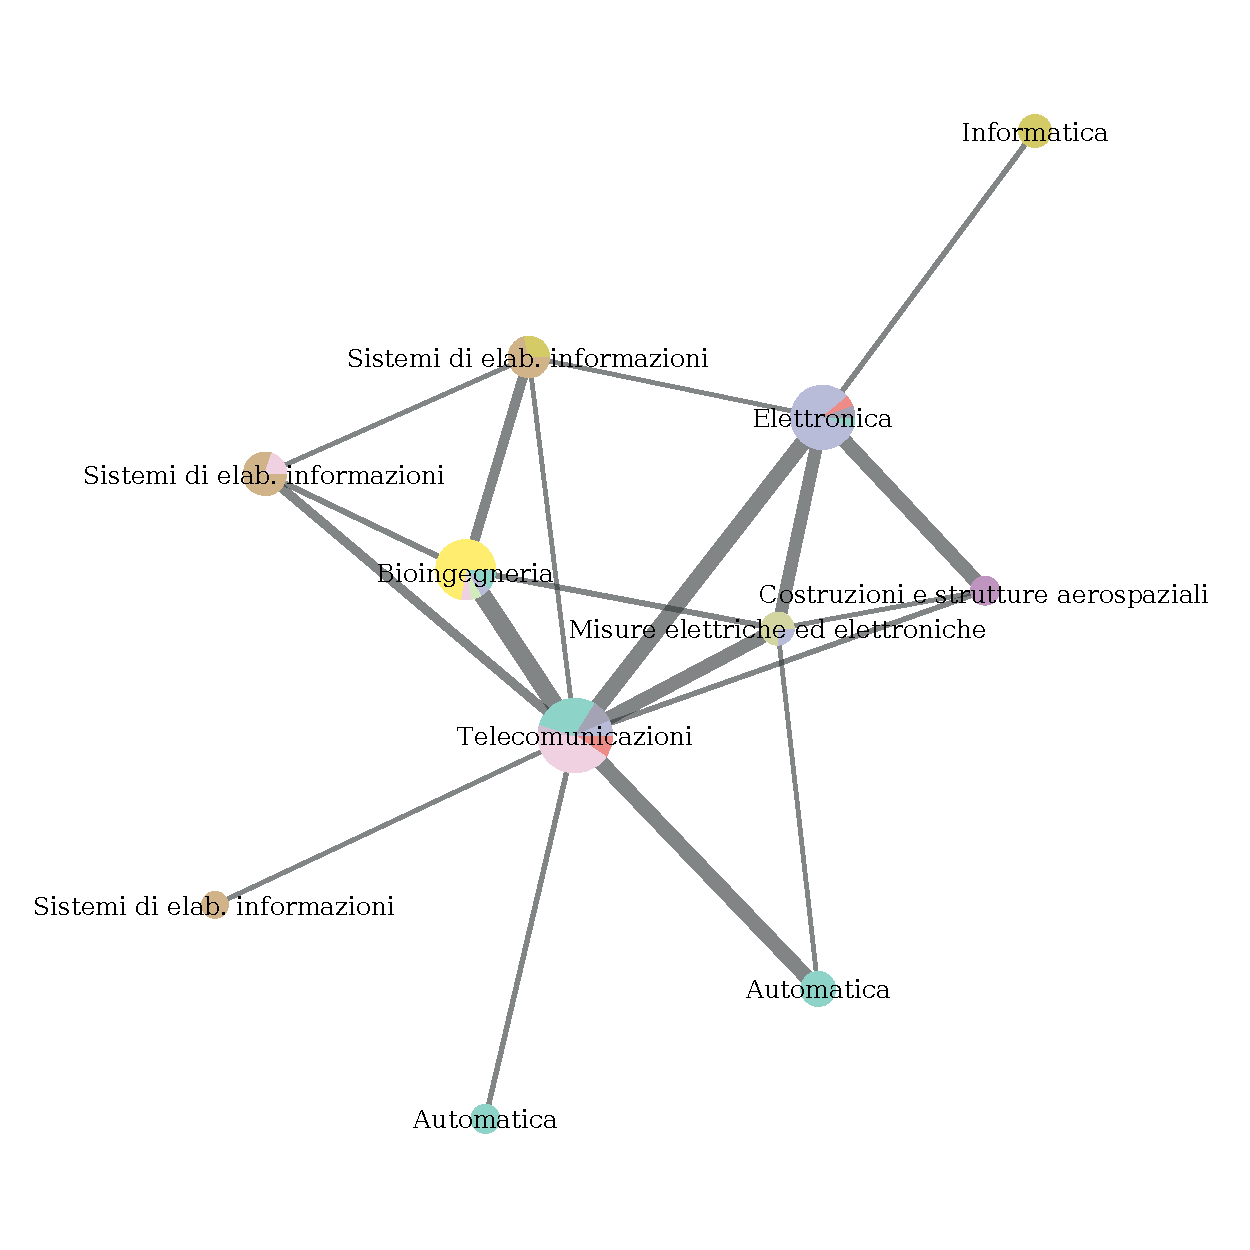
\includegraphics[page=1,scale=0.30]{img/Aggregati/GrafoAggregato_padovani_nomi_Zgirvnew_DEI.pdf}}
                \caption{Padovani - uniti per nome}
            \end{subfigure}
            \\
            \begin{subfigure}[b]{0.5\textwidth}
                \centering
                \setlength{\fboxrule}{0pt} % barbatrucco per far sparire il bordo della box
                \fbox{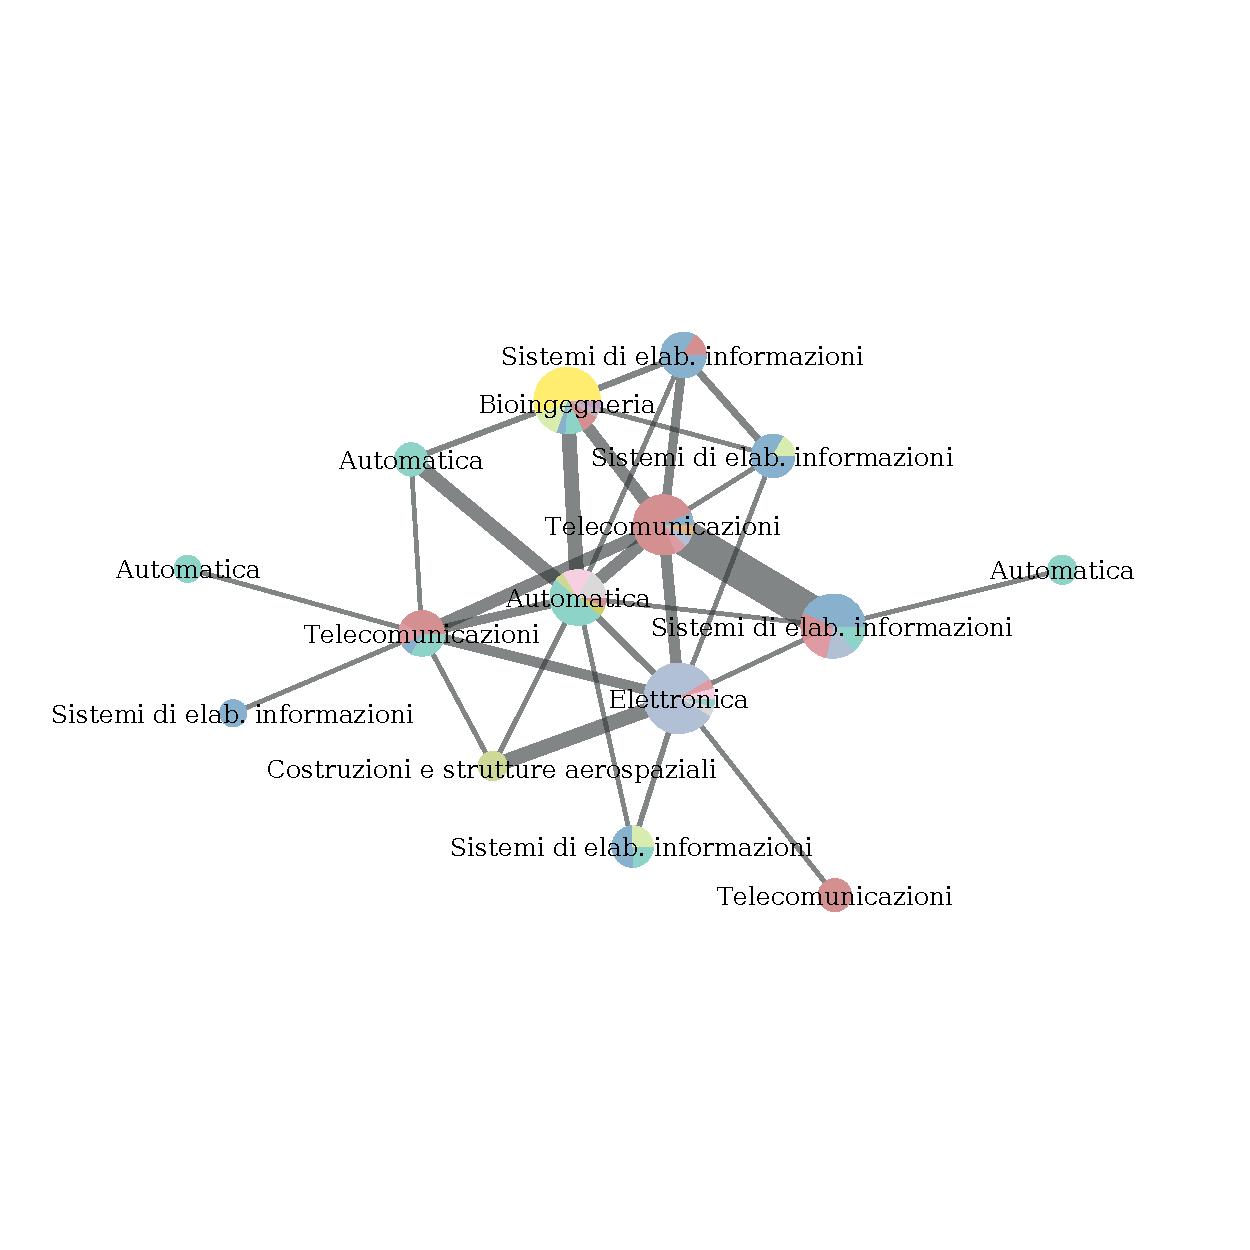
\includegraphics[page=1,scale=0.30]{img/Aggregati/GrafoAggregato_tutti_distanza_Zgirvnew_DEI.pdf}}
                \caption{Tutti - uniti per distanza}
            \end{subfigure}%
            ~
            \begin{subfigure}[b]{0.5\textwidth}
                \centering
                \setlength{\fboxrule}{0pt} % barbatrucco per far sparire il bordo della box
                % \fbox{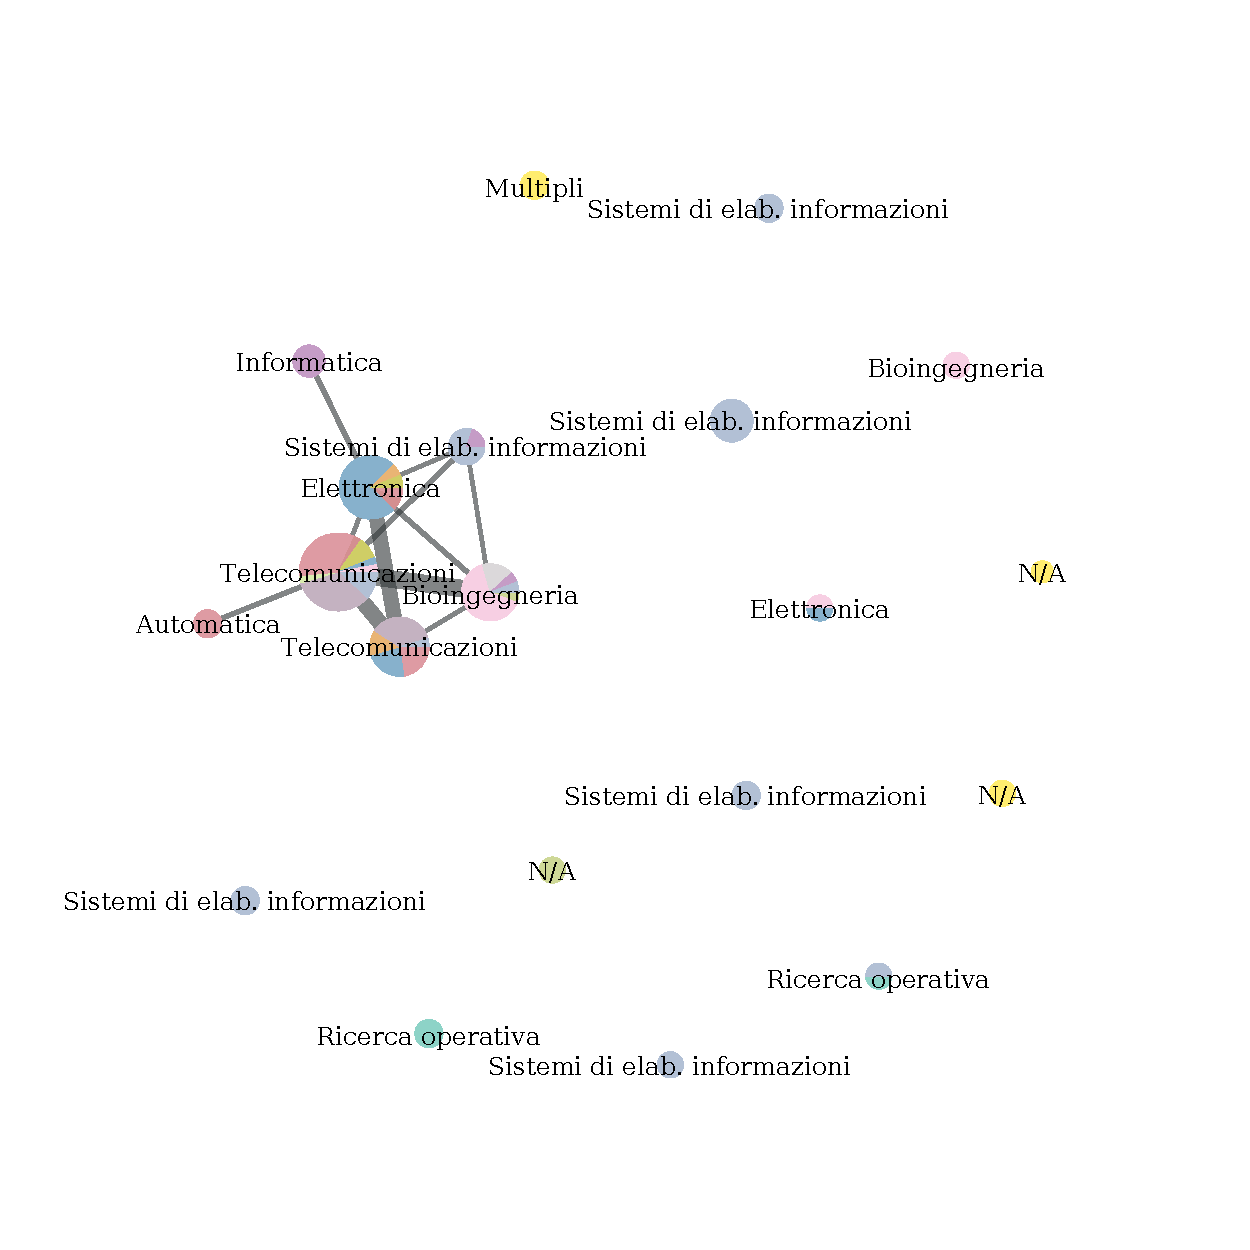
\includegraphics[page=1,scale=0.30]{img/Aggregati/GrafoAggregato_padovani_edge_clanemo_DEI.pdf}}
                \fbox{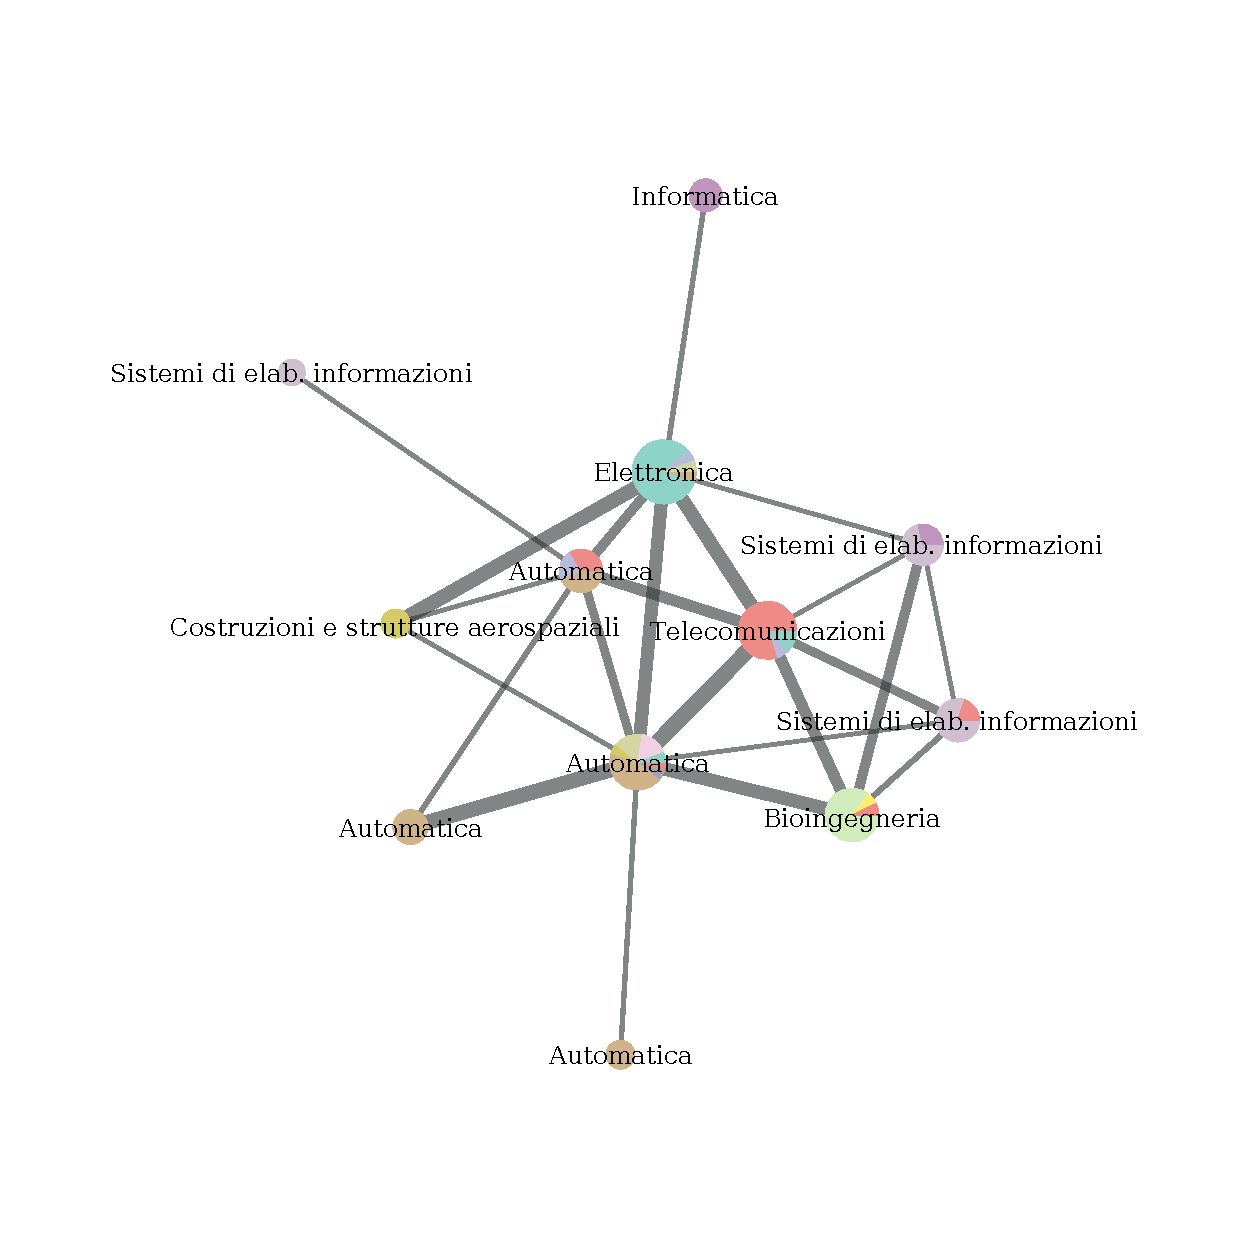
\includegraphics[page=1,scale=0.30]{img/Aggregati/GrafoAggregato_padovani_distanza_Zgirvnew_DEI.pdf}}
                \caption{Padovani - uniti per distanza}
            \end{subfigure}%
            \\
            \begin{subfigure}[b]{0.5\textwidth}
                \centering
                \setlength{\fboxrule}{0pt} % barbatrucco per far sparire il bordo della box
                \fbox{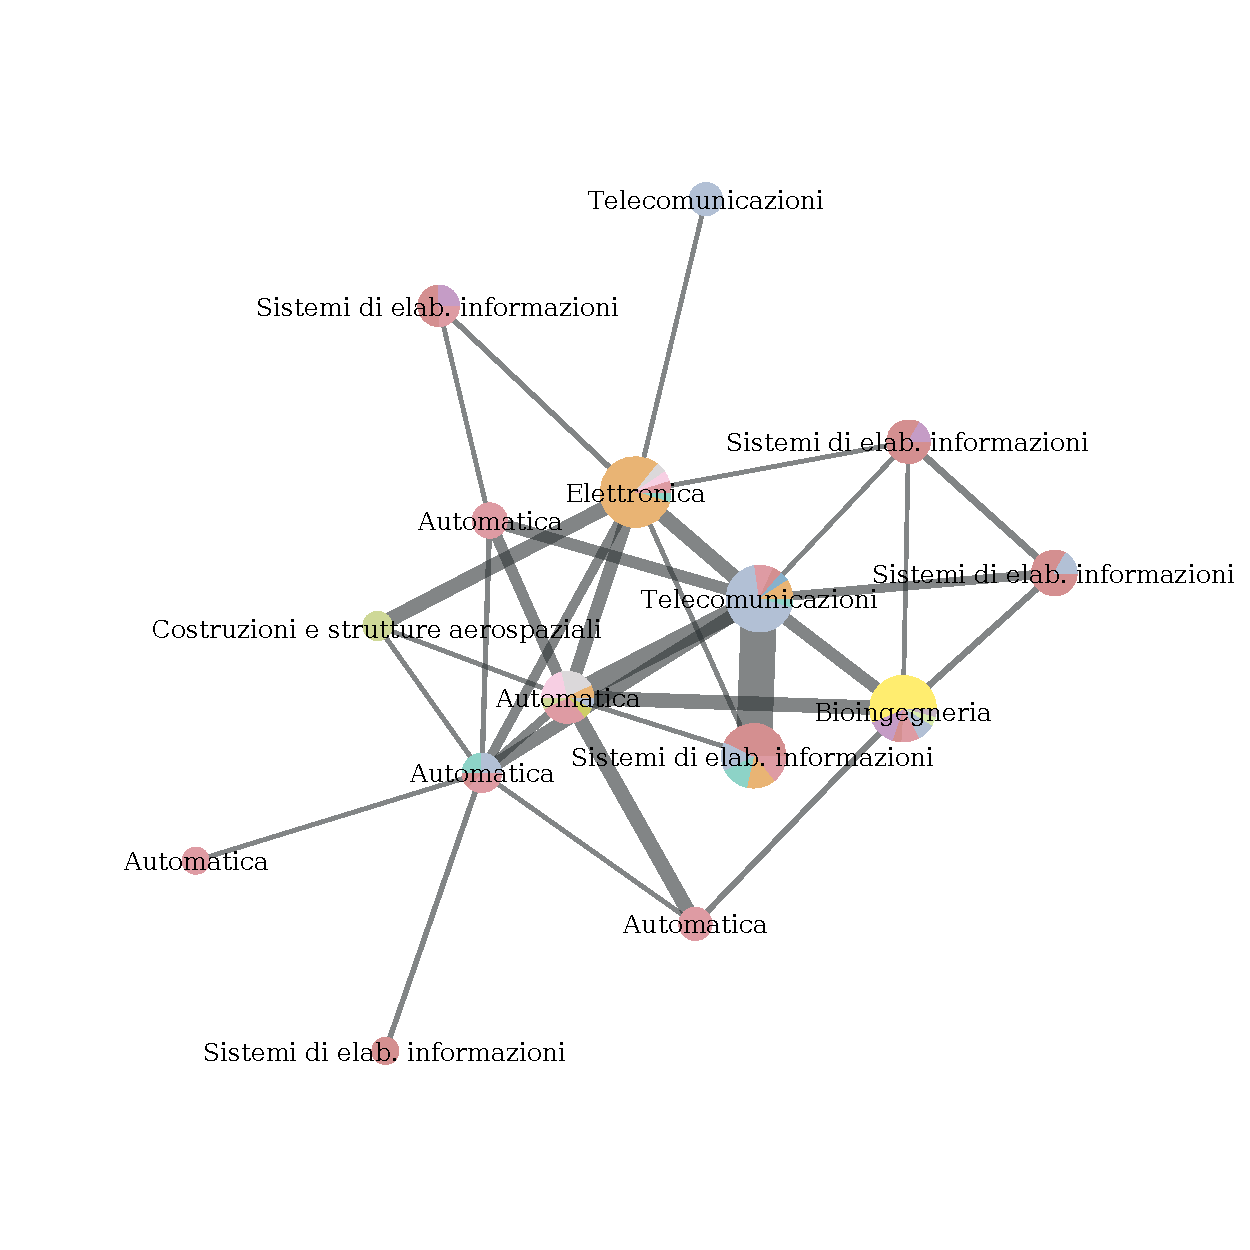
\includegraphics[page=1,scale=0.30]{img/Aggregati/GrafoAggregato_tutti_edge_Zgirvnew_DEI.pdf}}
                \caption{Tutti - uniti per nodi adiacenti}
            \end{subfigure}%
            ~
            \begin{subfigure}[b]{0.5\textwidth}
                \centering
                \setlength{\fboxrule}{0pt} % barbatrucco per far sparire il bordo della box
                \fbox{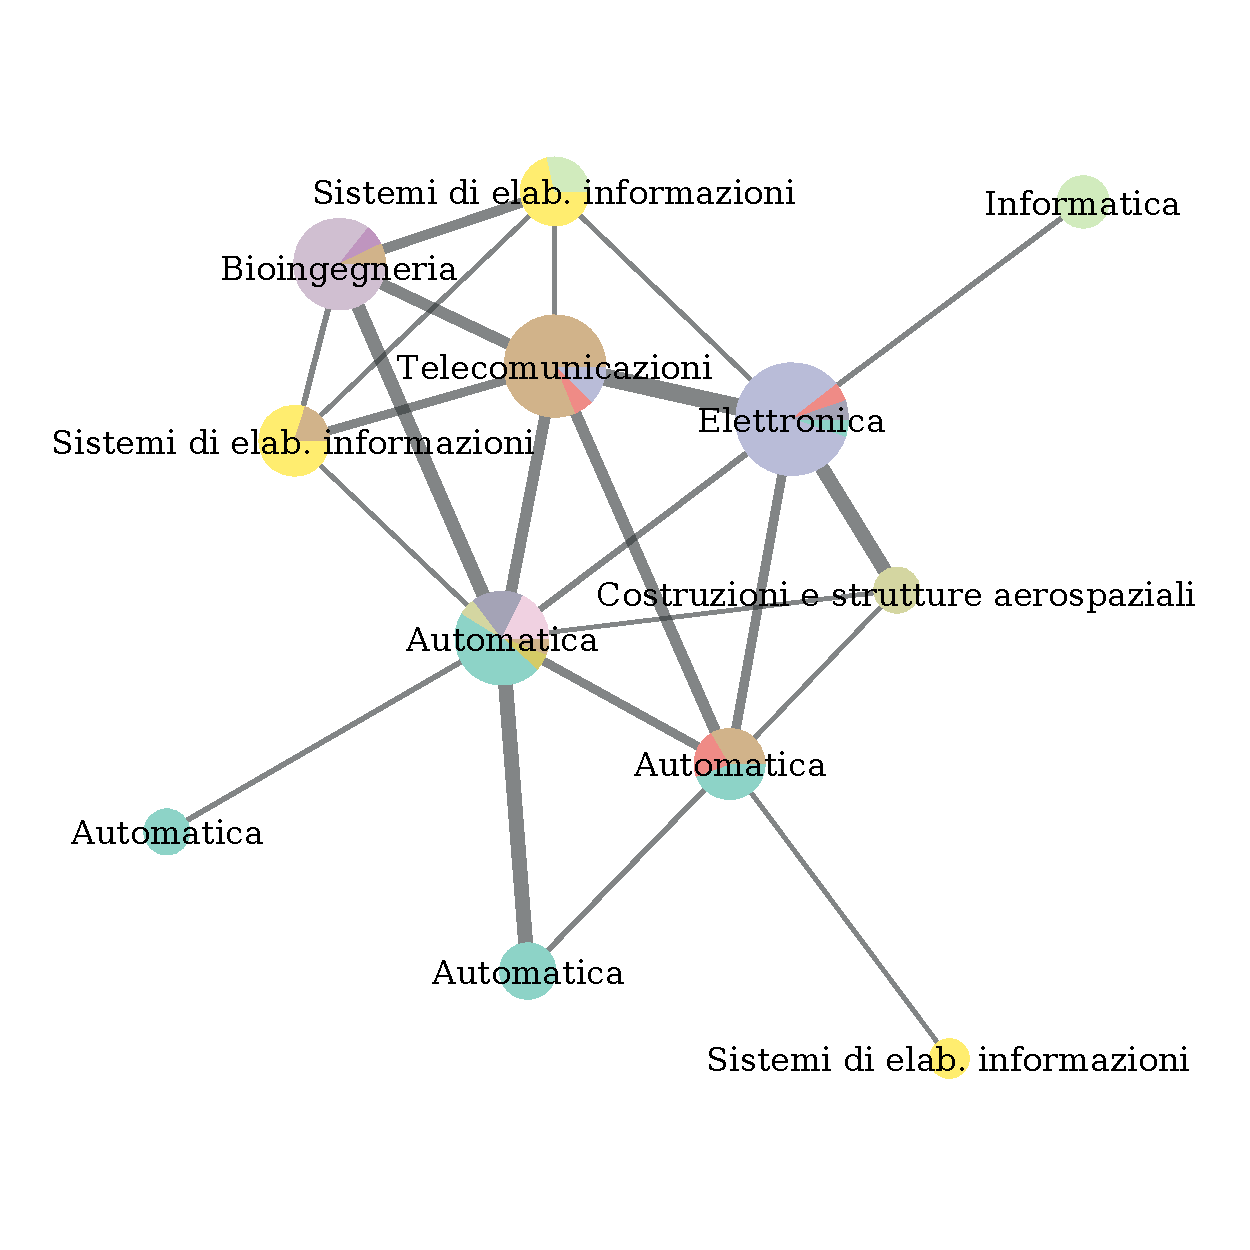
\includegraphics[page=1,scale=0.30]{img/Aggregati/GrafoAggregato_padovani_edge_Zgirvnew_DEI.pdf}}
                \caption{Padovani - uniti per nodi adiacenti}
        \end{subfigure}%
    \caption{Confronto delle suddivisioni in cluster generate dall'algoritmo Girvan-Newman applicato
    alla componente centrale del grafo; i cluster sono stati aggregati in nodi, i colori dei nodi
    indicano la suddivisione in classi dei cluster; l'etichetta corrisponde alla classe
    predominante nel cluster}
    \label{fig:grafigirvanaggregati}
\end{figure}

% \centerline{
% \begin{minipage}{1.20\textwidth}
% \setlength{\fboxrule}{0pt}	%barbatrucco per far sparire il bordo della box
% \fbox{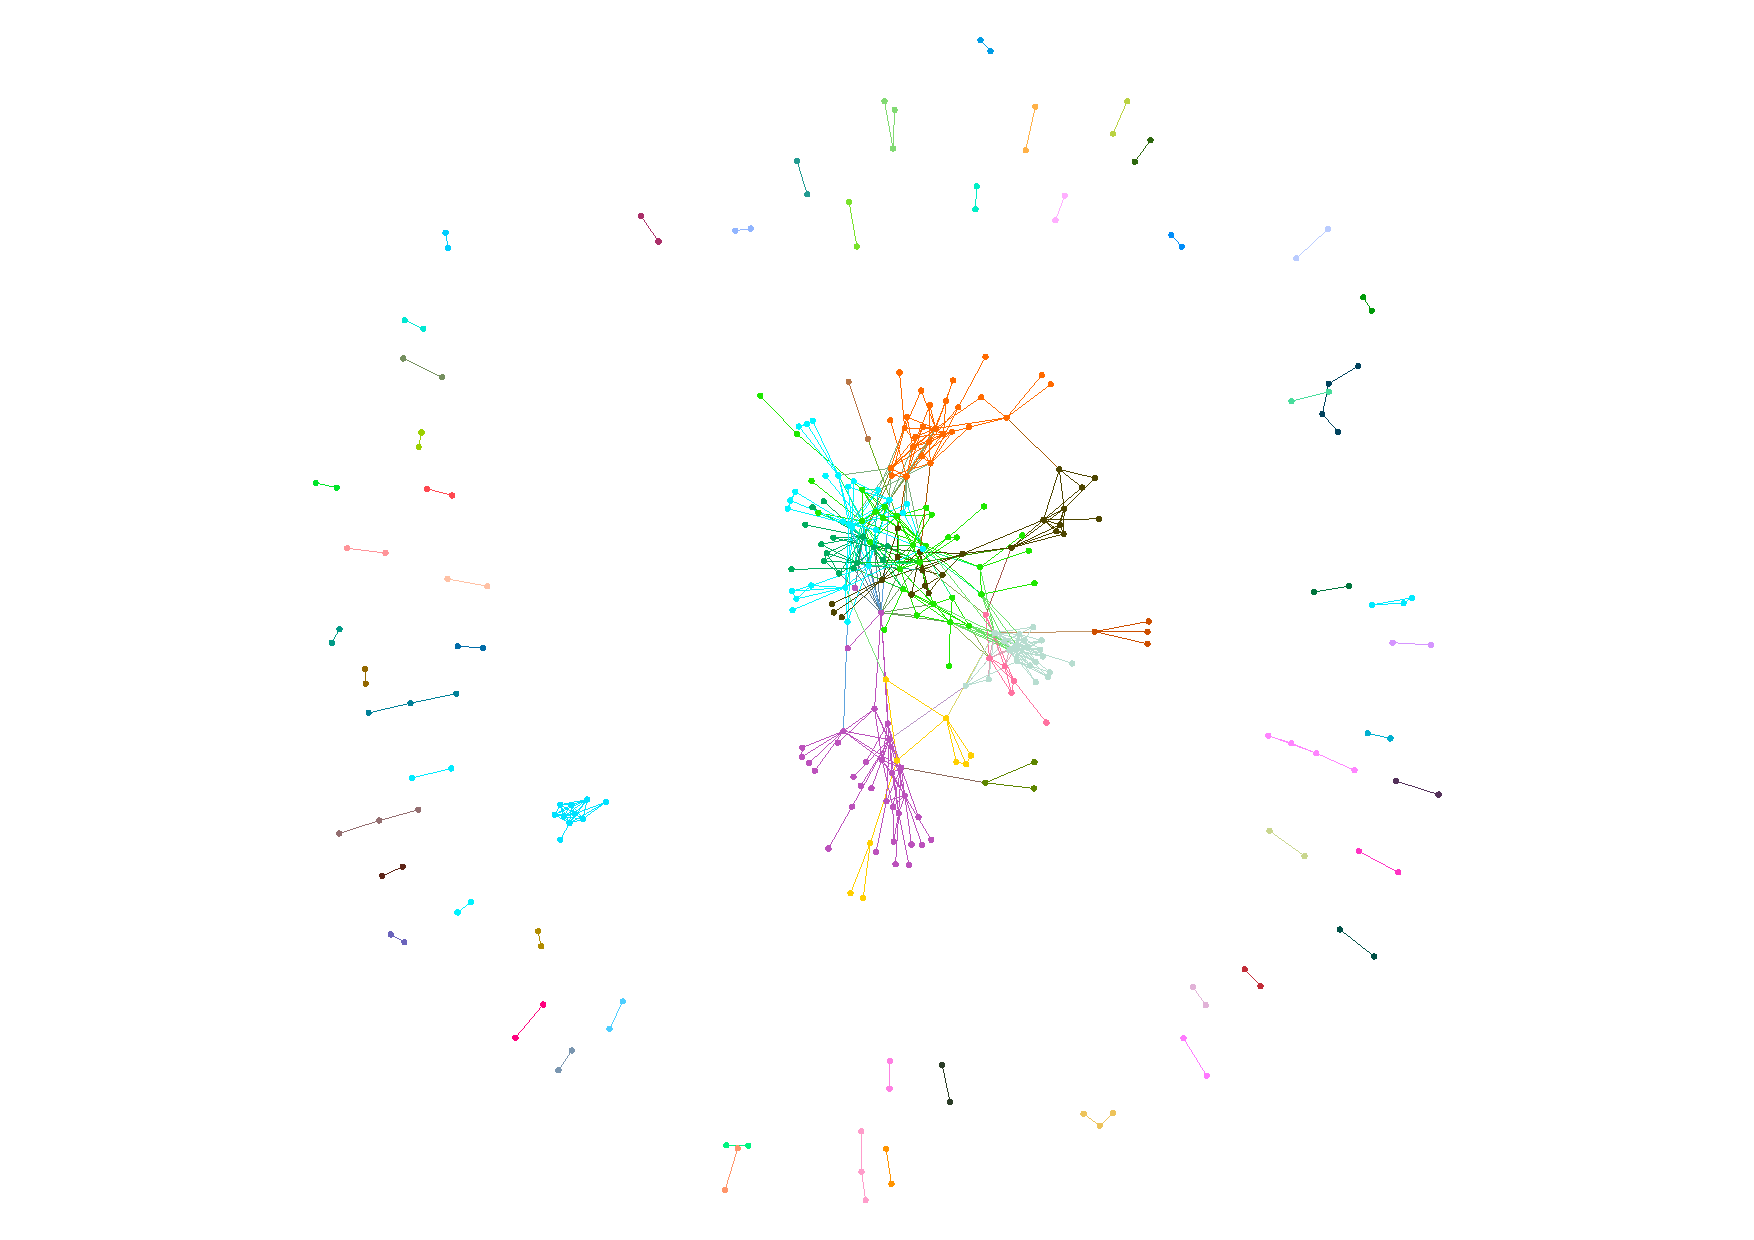
\includegraphics[page=1,scale=0.47]{img/GrafoTuttiDistanza23.pdf}}
% \captionof{figure}{Grafo collaborazioni unificati per distanza}
% \label{img:grafotuttidistanza}
% \end{minipage}
% }

% \subsubsection{Tutti vs padovani}\label{ssc:analisitp}
% Tra tutti e padovani c'è molta differenza.
% \subsubsection{Collassi vari}\label{ssc:analisicollassi}
% Tra le varie strade di collasso non c'è sostanziale differenza.
% \subsubsection{Metodi di community detection}\label{ssc:analisicd}
% Tra le varie comunità non c'è sostanziale differenza.

% TODO subsubsection su iterazioni collasso short path e perché non è vero

% TODO alcune strade sono migliori anche se la v-measure è simile

\whitePage
\chapter{Conclusioni} \label{cap:conclusioni}

Partendo da una lista di nomi di un dipartimento si può estrarre un grafo che lo rappresenti? Le
comunità generate rispecchiano quelle reali?

TODO se vuoi fallo su matematica e mostra un grafo con qualche valore di v-measure


%%% OBBLIGATORIA:


%::::::::::::::::::::::::::::::::::BIBLIOGRAFIA::::::::::::::::::::::::::::::::::::::::::::::::::::::

% \nocite{*} % visto che non ho citato niente serve per non offendere bibtex
\bibliographystyle{plainurl}
% sarebbe bello usare bibtex ma non funziona, o forse non lo so usare
% vedremo di imparare
\bibliography{tesiautnet} %%% nome file(s)

\end{document}

%::::::::::::::::::::::::::::::::::::::::::::::::::::::::::::::::::::::::::::::::::::::::::::::::::::
